\documentclass[a4,10pt,oneside,openany]{ctexart}
\usepackage[utf8x]{inputenc}
%\usepackage[UTF8]{ctex}
%\usepackage[english]{babel}
\usepackage{mathpazo}
\usepackage{mathrsfs}
\setlength{\parskip}{0.2\baselineskip}
%\setlength{\parskip}{0.2em}
\usepackage{url}
\usepackage{amssymb,amsmath,amsthm,amsfonts}
\usepackage{mathtools}
\usepackage{geometry}
\usepackage{float}
\usepackage{tikz}
\tikzset{elegant/.style={smooth,thick,samples=50,cyan}}
\tikzset{eaxis/.style={->,>=stealth}}


\usepackage{extarrows}
\usepackage{subfigure}
\usepackage{graphics}
\usepackage{wrapfig}
\usepackage{graphicx}
\usepackage{enumerate}
\usepackage{subfigure}
\usepackage{CJKulem}%中文删除线
\usepackage[normalem]{ulem} % \sout{想加删除线的中文}
\usepackage{picinpar}%图片绕排,是真滴烦
\usepackage{float}

%页眉页脚
\usepackage{authblk}
\usepackage{fancyhdr}
\usepackage{lastpage}

%以下是书写伪代码用
\usepackage{algorithm}  
\usepackage{algpseudocode}  
\renewcommand{\algorithmicrequire}{\textbf{Input:}}  % Use Input in the format of Algorithm  
\renewcommand{\algorithmicensure}{\textbf{Output:}} % Use Output in the format of Algorithm 

\geometry{a4paper, left=3cm, right=3cm, bottom=3cm, top=3cm}%此行定义了纸张大小和边距,不需要可删除

%以下是Inkspace
\usepackage{import}
\usepackage{xifthen}
\usepackage{pdfpages}
\usepackage{transparent}

\usepackage{verbatim}%comment 环境
%\usepackage[backref]{hyperref} %参考文献高亮跳转\\
\usepackage[colorlinks, linkcolor=black, anchorcolor=blue, citecolor=red]{hyperref}

\newcommand{\incfig}[1]{%
\def\svgwidth{\columnwidth}
\import{./figures/}{#1.pdf_tex}
}

\newtheorem{deff}{定义}[section]
\newtheorem{thm}{定理}[section]
\newtheorem{clm}[thm]{命题}
\newtheorem{lemma}[thm]{引理}
\newtheorem{prf}{证明}[section]


\renewcommand{\proofname}{\indent Pr}
\renewcommand{\qedsymbol}{$\blacksquare$}    % 证毕符号改成黑色的正方形

\newcommand{\argmin}[1]{\underset{#1}{\arg \min}\ }
\newcommand{\ceil}[1]{\left\lceil #1 \right \rceil }
\newcommand{\norm}[1]{\left \Vert #1 \right \Vert}
\newcommand{\tform}[1]{\left \Vert #1 \right \Vert_2}
\newcommand{\tnorm}[1]{\left \Vert #1 \right \Vert_2}
\newcommand{\onorm}[1]{\left \Vert #1 \right \Vert_1}
\newcommand{\abs}[1]{\left|#1 \right|}
\newcommand{\var}[1]{\text{Var}\left[ #1\right]}
\newcommand{\xk}[1]{\left( #1\right)} 
\newcommand{\zk}[1]{\left[ #1\right]} 
\newcommand{\dk}[1]{\left\{ #1\right\}} 
\newcommand{\bd}[1]{\bold{#1}}

%量子力学符号------
\newcommand{\xde}{\text{Schrödinger}}
\newcommand{\avg}[1]{\left \langle #1 \right \rangle}
\newcommand{\lvec}[1]{\left \langle #1 \right |}
\newcommand{\rvec}[1]{\left | #1 \right \rangle}


\newtheorem{lproof}{证明}[section]
\newtheorem{tuilun}{推论}
\newtheorem{eg}{例}[section]
\newtheorem{solve}{解}[section]
\newcommand\ii{\textup{i}}
\newcommand\dd{\mathrm{d}}


%自定义数学符号
\newcommand{\diag}{\textup{diag}}
\newcommand{\Frobenius}[1]{\left\Vert #1 \right\Vert}
\newcommand{\fform}[1]{\left\Vert #1 \right\Vert_F}
\newcommand{\parr}[2]{\frac{\partial #1}{\partial #2}}%一阶偏微分
\newcommand{\parrr}[2]{\frac{\partial^2 #1}{\partial #2^2}}%二阶偏微分
\newcommand{\lap}[1]{\parrr{#1}{x} + \parrr{#1}{y} = 0}%二元拉普拉斯方程
\newcommand{\ddd}[2]{\frac{\textup{d} #1}{\textup{d} #2}}%微商
\newcommand{\dddd}[2]{\frac{\textup{d}^2 #1}{\textup{d} #2^2}}%微商

%二重以上环路积分,强迫症了属于是
\def\ooint{{\bigcirc}\kern-11.5pt{\int}\kern-6.5pt{\int}}
\def\oooint{{\bigcirc}\kern-12.3pt{\int}\kern-7pt{\int}\kern-7pt{\int}}


\newcommand{\tu}{\textup}
\newcommand{\bm}{\boldsymbol}
\newcommand{\ol}[1]{$\overline{#1}$}
\newcommand{\re}[1]{\textup{Re}(#1)}
\newcommand{\im}[1]{\textup{Im}(#1)}
\newcommand{\fa}{\forall}
\newcommand{\ex}{\exists}
\newcommand{\st}{\textup{  s.t. }}
\newcommand{\ve}{\varepsilon}
\newcommand{\disp}{\displaystyle}
\newcommand{\chj}{\textup{Cauchy}积分公式}
\newcommand{\res}[1]{\textup{Res}\left(#1\right)}
\newcommand{\mysum}[1][n]{\sum_{i = 1}^{#1}}%求和
\newcommand{\series}[1]{\sum_{n = 0}^{\infty} #1_{n}}%级数
\newcommand{\seriesa}[1]{\sum_{n = 0}^{\infty} \left| #1_{n}\right|}%绝对级数
\newcommand{\fseries}[1]{\sum_{k = 1}^{\infty} #1_k (z)}

\newcommand*{\num}{pi}

%书写横线
\newcommand{\horrule}[1]{\rule[0.5ex]{\linewidth}{#1}} 	% Horizontal rule

% 文档标题
\title{
{\normalfont\normalsize\textsc{
Peking University\\
Introduction to Computer Vision, Spring 2024 \\[25pt]}}
\horrule{0.5pt}\\
\sffamily{Introduction to Computer Vision\\Course Notes}\\
\horrule{1.8pt}\\[20pt]
}

% 作者和联系方式
\author[1]{Prof. He Wang\thanks{https://hughw19.github.io/}}
\author[2]{林晓疏\thanks{wangyuanqing@pku.edu.cn}}
\author[2]{Yutong Liang\thanks{lyt0112@outlook.com}}
\affil[1]{主讲教师}
\affil[2]{笔记整理}

% 文档日期
\date{\today}

\pagestyle{fancy}
\fancyhf{}
\fancyhead[L]{\leftmark}  % 在页眉左侧显示章节名
\fancyfoot[C]{\thepage}  % 在页脚中间显示页码


\begin{document}
	\maketitle
	\section*{前言}

这本笔记是作者于2022年春信息科学技术学院王鹤老师开设的计算机视觉导论课程期间的笔记.王鹤老师在Stanford获得Ph.D学位,课程中也毫不令人意外地带有许多\href{https://cs231n.github.io/}{CS231n: Convolutional Neural Network for Visial Recognition}和\href{https://web.stanford.edu/class/cs231a/course_notes.html}{CS231A: Computer Vision, From 3D Reconstruction to Recognition}等课程的影子.课程从对计算机视觉领域的传统方法的介绍开始,介绍了CNN和诸多深度学习的基本知识,如BatchNorm,Regularization等.随后进入3D视觉部分,详细介绍了Pinhole Camera这一模型以及相机标定,对极几何等相关知识.期中之后转入3D数据,语义分割,物体位姿判定以及RNN和生成模型部分.

笔记主要是对王鹤老师上课内容的记录,部分内容由笔者在课余时间了解后添加,这些内容都给出了参考文献或链接.除此之外,笔者还依惯例添加了几节附录,以补充正文当中一些没有展开的细节,以供参考.

这门课是笔者三年以来在信科上过的水准最高的课程,无论是课程内容,教师讲授水平,作业质量,考试区分度还是答疑,都是笔者体验过的课程中最高水准的一档.若信科未来能有一半专业课能达到本课的水平,则世界一流大学指日可待 (.

最后,感谢王鹤老师和张嘉曌,陈嘉毅两位助教.笔者曾多次向张助教询问问题,均得到了细致的回答,在此一并表示感谢.

\rightline{林晓疏}

\rightline{2022年春}

作为北京大学信息科学技术学院的学生,长期以来饱受糟糕课程质量、糟糕课程作业、糟糕考试难度的折磨.
比如算法设计与分析的等课程的教学质量极低,教考分离,ICS考试一面黑板的考试错误题目订正等等.
在这样的环境下,幸运地遇到了王鹤老师开设的计算机视觉导论课程,内容丰富,作业质量高,考试难度适中,
绝对称得上是精品课程\sout{(与算分这种国家精品课程相区别)}.

王鹤老师将计算机视觉的发展脉络呈现给大家,在这个深度学习时代,
老师并没有完全忽视传统CV的方法,而是挑选了其中具有代表性的工作,这些工作为深度学习时代的CV打下了良好的基础,提供了许多基础工具和数据集的构建方式.
同时老师也更加注重深度学习的基础知识,如 BatchNorm 的特性和与其他 Norm 的区别,许多人仅仅只是会 PyTorch 的积木搭建,但是对于这些基础知识的原理和性质却不甚了解,
导致在实际使用中遇到问题时无法解决,王老师在这方面往往提出 intuitive 的问题,引人深思.

我是在大三下学期选修了这门课程,即使我已经具有了一定的深度学习基础,但是我仍然很享受上课\sout{看回放}的过程,因为对于许多已经了解的知识,王老师会再度给出解释,
总是让我在同一个地方有不同的收获.

我在本学期期中考试之前偶然了解到曾经有学长撰写了一本笔记,但是许多内容已经进行了更新或者删改,因此我联系上林晓疏(笔名)学长,获取了这份笔记的源代码,
并在此基础上进行更新,以飨后人.

该笔记按照讲授先后顺序进行排列,但是章节编排按照知识结构划分,因此章节划分可能与课程进度有所不同.
同时本笔记不能替代课程,只是对这部分知识的总结和思考,建议与课程回放配合食用.

\rightline{Yutong Liang}
\rightline{2024年4月24日}

	\clearpage
	\tableofcontents
	\section{Edge Detection}

\subsection{What is an Edge?}

“边缘”是图像中的一个区域,在这个区域中,沿着图像的一个方向,
像素强度值 (或者说对比度) 发生了“显著”的变化,而在其正交方向上,
像素强度值 (或对比度) 几乎没有变化.

\subsection{Criteria for Optimal Edge Detection}

\begin{equation}
\text{Accuracy}=\frac{\text{TP}+\text{TN}}{\text{TP}+\text{FP}+\text{TN}+\text{FN}} 
\end{equation}

\begin{equation}
\text{Precision}=\frac{\text{TP}}{\text{TP}+\text{FP}} 
\end{equation}

\begin{equation}
\text{Recall}=\frac{\text{TP}}{\text{TP}+\text{FN}}
\end{equation}

Precision 和 Recall 都代表着你检测出的真正边缘所占比例,但是 Precision 的分母
是你检测出的边缘,Recall 的分母是真正的边缘.

\subsection{Non-Maximal Suppression (NMS)}

非最大值抑制,顾名思义,就是抑制非最大值,这里的最大值指的是梯度的局部最大值.

在计算出了所有点的梯度之后,会有很多像素的梯度大于设定的阈值,而我们希望最后得出的边缘像素真的看起来
像一条线而不是一块区域,所以 NMS 的目的是为了抑制那些不是边缘的像素,只保留那些是边缘的像素。

\begin{figure}[htbp]
    \centering
	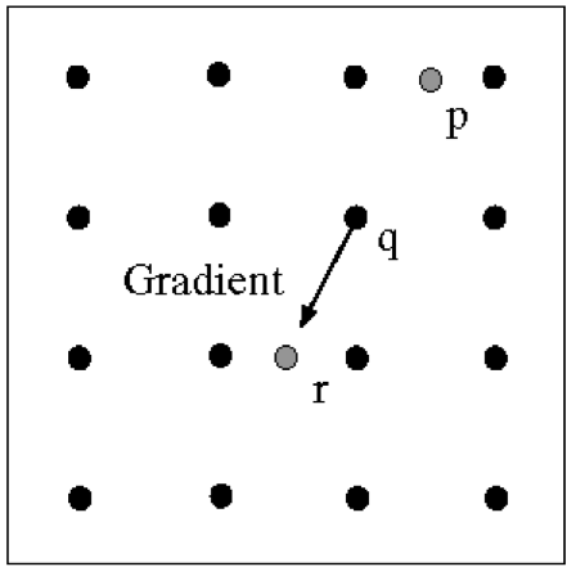
\includegraphics[scale=0.2]{figures/NMS.png}
	\caption{NMS示意图}
\end{figure}

对于一个边缘像素的候选点,我们认为它是边缘当:它比它梯度方向的两个点 $q+\nabla q$ 和 $q-\nabla q$ 的梯度值大,
也就是这个点的梯度大小是局部最大值的时候.

\begin{figure}[htbp]
    \centering
	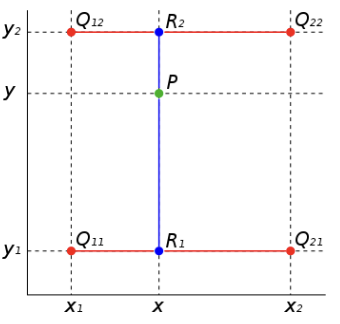
\includegraphics[scale=0.4]{figures/bilinear.png}
	\caption{双线性插值}
\end{figure}

计算这个点梯度方向的点的梯度值可以使用双线性插值法,就是把这个点周围的四个点的梯度按照横纵距离反比加权.

当然,NMS 是一个思想而不是针对边缘检测的算法,比如对于 keypoint detection,object detection (like YOLO) 都可以使用 NMS,
实现的思路都很类似,使用一个打分函数看这个备选点 (bounding box) 是不是比跟它相邻 (冲突) 的点 (bounding box) 好,如果是就保留,否则就抑制.

\subsection{A Simplified Version of NMS}

\begin{figure}[htbp]
    \centering
	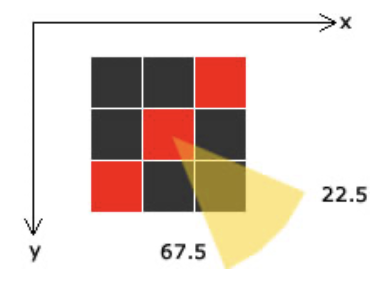
\includegraphics[scale=0.55]{figures/simple_NMS.png}
	\caption{简化版本的双线性插值}
\end{figure}

一个 NMS 的简化版本是把双线性插值省去,直接让这个像素的梯度大于它梯度方向的那两个相邻像素的梯度.

\subsection{Hysteresis Thresholding}

使用高阈值 (maxVal) 开始边缘曲线,使用低阈值 (minVal) 继续它们。

\begin{itemize}
    \item Pixels with gradient magnitudes > maxVal should be reserved.
    \item Pixels with gradient magnitudes < minVal should be removed.
\end{itemize}

How to decide maxVal and minVal? Examples:

\begin{itemize}
    \item maxVal = 0.3 $\times$ average magnitude of the pixels that pass NMS
    \item minVal = 0.1 $\times$ average magnitude of the pixels that pass NMS
\end{itemize}

	\chapter{Keypoint Detection}
(Corner Detection)

\begin{introduction}[Keywords]
    \item 角点检测 Corner Detection
    \item 结构张量 Structure Tensor
    \item 特征值分解 Eigenvalue Decomposition
    \item 等变性 Equivariance
    \item 尺度不变性 Scale Invariance
    \item Harris-Laplacian 检测器
    \item 高斯差分 Difference-of-Gaussians (DoG)
\end{introduction}

\begin{problem}
    What Points are Keypoints?
\end{problem}

\begin{enumerate}
    \item Repeatability: 可以在不同的图像中找到相同的点
    \item Saliency: 有趣的点
    \item Quantity: 量大管饱
    \item Accurate localization: 精确定位
\end{enumerate}
Corners 就是这样的 keypoints.




\section{The Basic Idea of Harris Corner}

\begin{figure}[htbp]
    \centering
    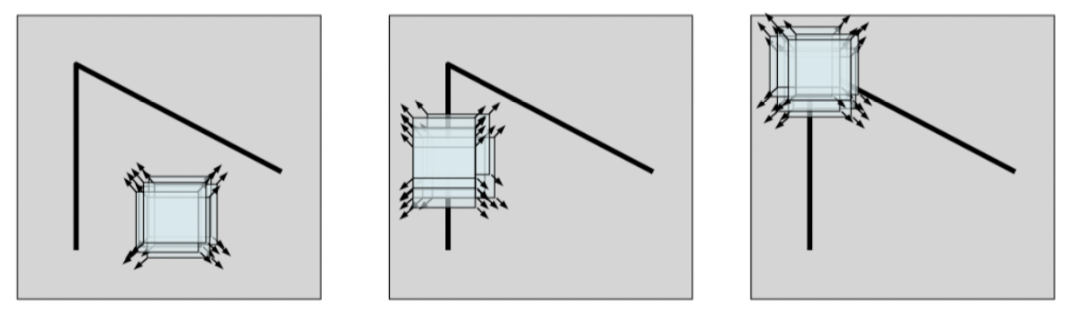
\includegraphics[width=0.8\textwidth]{figures/window_moving.png}
    \caption{移动窗口}    
\end{figure}

Move a window and explore intensity changes within the window.

Corner : significant change in all directions.

\section{Harris Corner}

一个 window,给定它的移动方向 $(u,v)$:

\begin{equation}
    \begin{aligned}
    E(u,v) &= \sum_{x,y} w(x,y) [I(x+u,y+v) - I(x,y)]^2\\
    &\approx \sum_{x,y} w(x,y) [I(x,y) + uI_x + vI_y - I(x,y)]^2\\
    &= \sum_{x,y} w(x,y) [uI_x + vI_y]^2\\
    &= w \ast \begin{bmatrix} u & v \end{bmatrix} \begin{bmatrix} I_x^2 & I_xI_y \\ I_xI_y & I_y^2 \end{bmatrix} \begin{bmatrix} u \\ v \end{bmatrix}\\
    &= \begin{bmatrix} u & v \end{bmatrix} \begin{bmatrix} w \ast I_x^2 & w \ast I_xI_y \\ w \ast I_xI_y & w \ast I_y^2 \end{bmatrix} \begin{bmatrix} u \\ v \end{bmatrix}\\
    &= \begin{bmatrix} u & v \end{bmatrix} R^{-1} \begin{bmatrix} \lambda_1 & 0\\ 0 & \lambda_2 \end{bmatrix} R \begin{bmatrix} u \\ v \end{bmatrix}\\
    &= \lambda_1 u_R^2 + \lambda_2 v_R^2
    \end{aligned}
\end{equation}

根据这两个特征值的大小可以判断这个点是不是角点.

\begin{figure}[htbp]
    \centering
    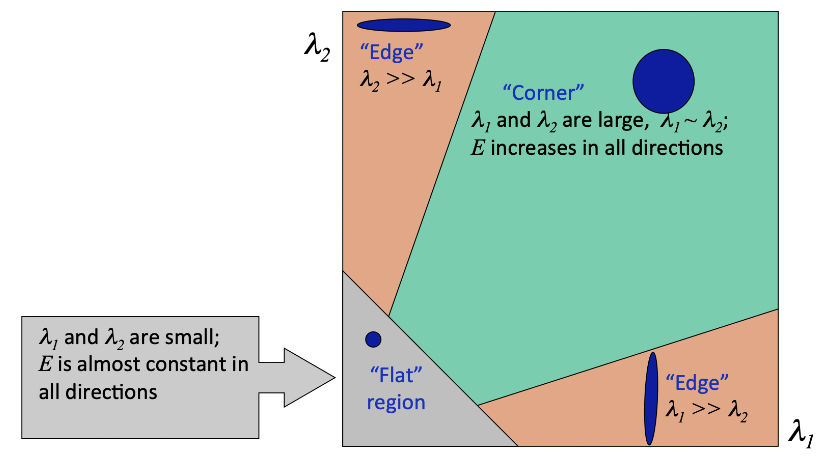
\includegraphics[width=0.6\textwidth]{figures/corner_map.png}
    \caption{特征值大小和这个点的是什么种类的点的关系}
\end{figure}
\begin{proposition}
    

这个点是角点一般需要满足:

\begin{itemize}
    \item $\lambda_1, \lambda_2>b$
    \item $\frac{1}{k}<\frac{\lambda_1}{\lambda_2}<k$
\end{itemize}

一个快速的判断公式:

\begin{equation}
\begin{aligned}
\theta&=\frac 12(\lambda_1\lambda_2-\alpha(\lambda_1+\lambda_2)^2)+\frac12(\lambda_1\lambda_2-2t)\\
&=\lambda_1\lambda_2-\alpha(\lambda_1+\lambda_2)^2-t\\
&=\det(R)-\alpha\text{Trace}(R)^2-t
\end{aligned}
\end{equation}

其中 $\alpha\in[0.04,0.06], t\in[0.01,0.03]$.

如果 $\theta$ 大于阈值, 则认为这个点是角点.
\end{proposition}
\begin{note}
Harris Corner 对平移和图像旋转是 equivariant的,对规模不是 equivariant 的.

为实现 rotation invariance, 可以用 Gaussian filter 来平滑图像, 使得角点不会因为旋转而改变.
\end{note}
\section{equivariant V.S. invariant}
\begin{definition}
    

\textbf{等变 (equivariant)}: $F(TX)=T(F(x))$,对于translation和rotation是等变的.

\textbf{不变 (invariant)}: $F(T(X))=F(X)$,也就是对于不同位置导出的角点还是那样,所以其实我们想要的是等变,也就是对于不同位置导出的角点做了同样的变化.
\end{definition}

\begin{problem}
    How to prove Harris detector is equivariant?
\end{problem}


只要说明角点检测函数也是equivariant即可.

角点检测函数包括了求导和卷积两个操作,显然求导是equivariant的,因为导数会随着trans和rot做相同的变化.

很有趣的是卷积也是equivariant的:当你的filter function是各向同性的,那么这个卷积就是equivariant的;但是如果是一个椭圆形的window,那这个卷积就不是equivariant的了.

\begin{figure}[htbp]
    \centering
    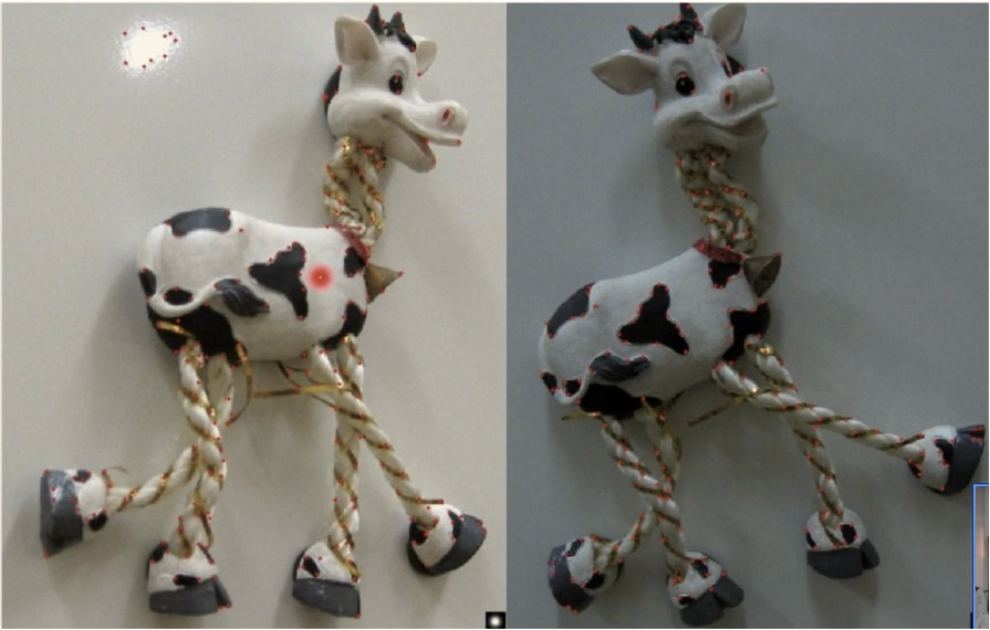
\includegraphics[width=0.6\textwidth]{figures/light_invariant.png}
    \caption{Illumination invariant}
\end{figure}
\begin{remark}
    这个高光说明不是环境 Illumination Invariant的
\end{remark}


\begin{problem}
    How to do NMS with corner-response-function?
\end{problem}


一个简单的想法:

先给出一个阈值,把所有response排序,成为一个list,从上到下按顺序把这个pixel周围的大于阈值的踢出list.
这个跟之前的NMS区别在于之前需要一条边,现在只需要一个点,那么现在比之前踢出的像素点更多.

\section{Scale Invariant Detectors}

这个不讲了?下次看看

Harris-Laplacian, SIFT (Lowe)
	\section{Line Fitting}

\subsection{Least Square Method}

\begin{figure}[htbp]
    \centering
    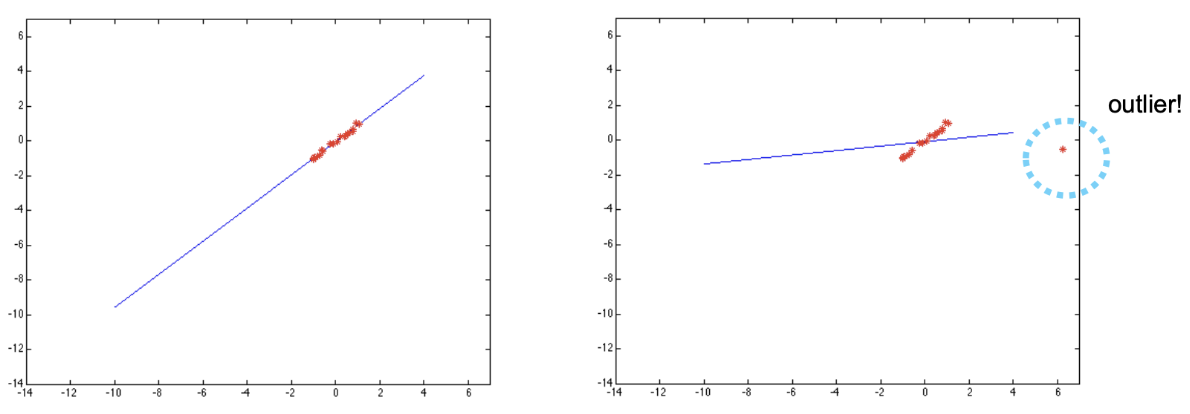
\includegraphics[width=0.8\textwidth]{figures/not_roboust_outliner.png}
    \caption{Least Square Method is not robust to outliers}
\end{figure}

Robust to small noises but sensitive to outliers.

\subsection{RANSAC}

RANSAC:RANdom SAmple Consensus

Idea: we need to find a line that has the largest supporters (or inliers)

RANSAC loop:

假设这个直线 (平面) 需要两个 (n个) 点来确定.

\begin{enumerate}
    \item 随机选择 k 组能确定这个直线的点,也就是在所有点里面选出一个 $k\times 2$ 的矩阵
    \item 对每一组点计算出一条直线
    \item 对每一组点的直线计算出所有点到这条直线的距离,如果小于阈值,则认为这个点是这条直线的 inlier
    \item 找到最大的 inlier 数量的直线,如果大于阈值,则认为这条直线是最优的
    \item 对这个最优的直线,用这个直线所有的 inlier 重新计算一次直线
\end{enumerate}

\subsection{RANSAC calculation}

假设我们有所有 inliner 占比为 $w$ 的先验知识,同时希望有不低于 $p$ 的概率能够找到一个最优的直线,那么我们需要多少次迭代呢?

\begin{equation}
\mathbf{\Pr}\text{[一组点全部是inliner]} = w^n
\end{equation}

如果一组点中有一个点是 outliner,那么我们称这组点 fail.

\begin{equation}
\mathbf{\Pr}\text{[k组点全部fail]} = {(1-w^n)}^k
\end{equation}

我们希望 k 组点全部 fail 的概率小于 $1-p$.

\begin{equation}
{(1-w^{n})}^k < 1-p
\Rightarrow
k > \frac{\log(1-p)}{\log(1-w^n)}
\end{equation}

\subsection{Hough Transform}

其实就是把一条直线从实际空间的表示转换到参数空间的表示.但是如果存在垂直的直线,可能需要考虑使用极坐标来作为参数空间.

\begin{figure}[htbp]
    \centering
    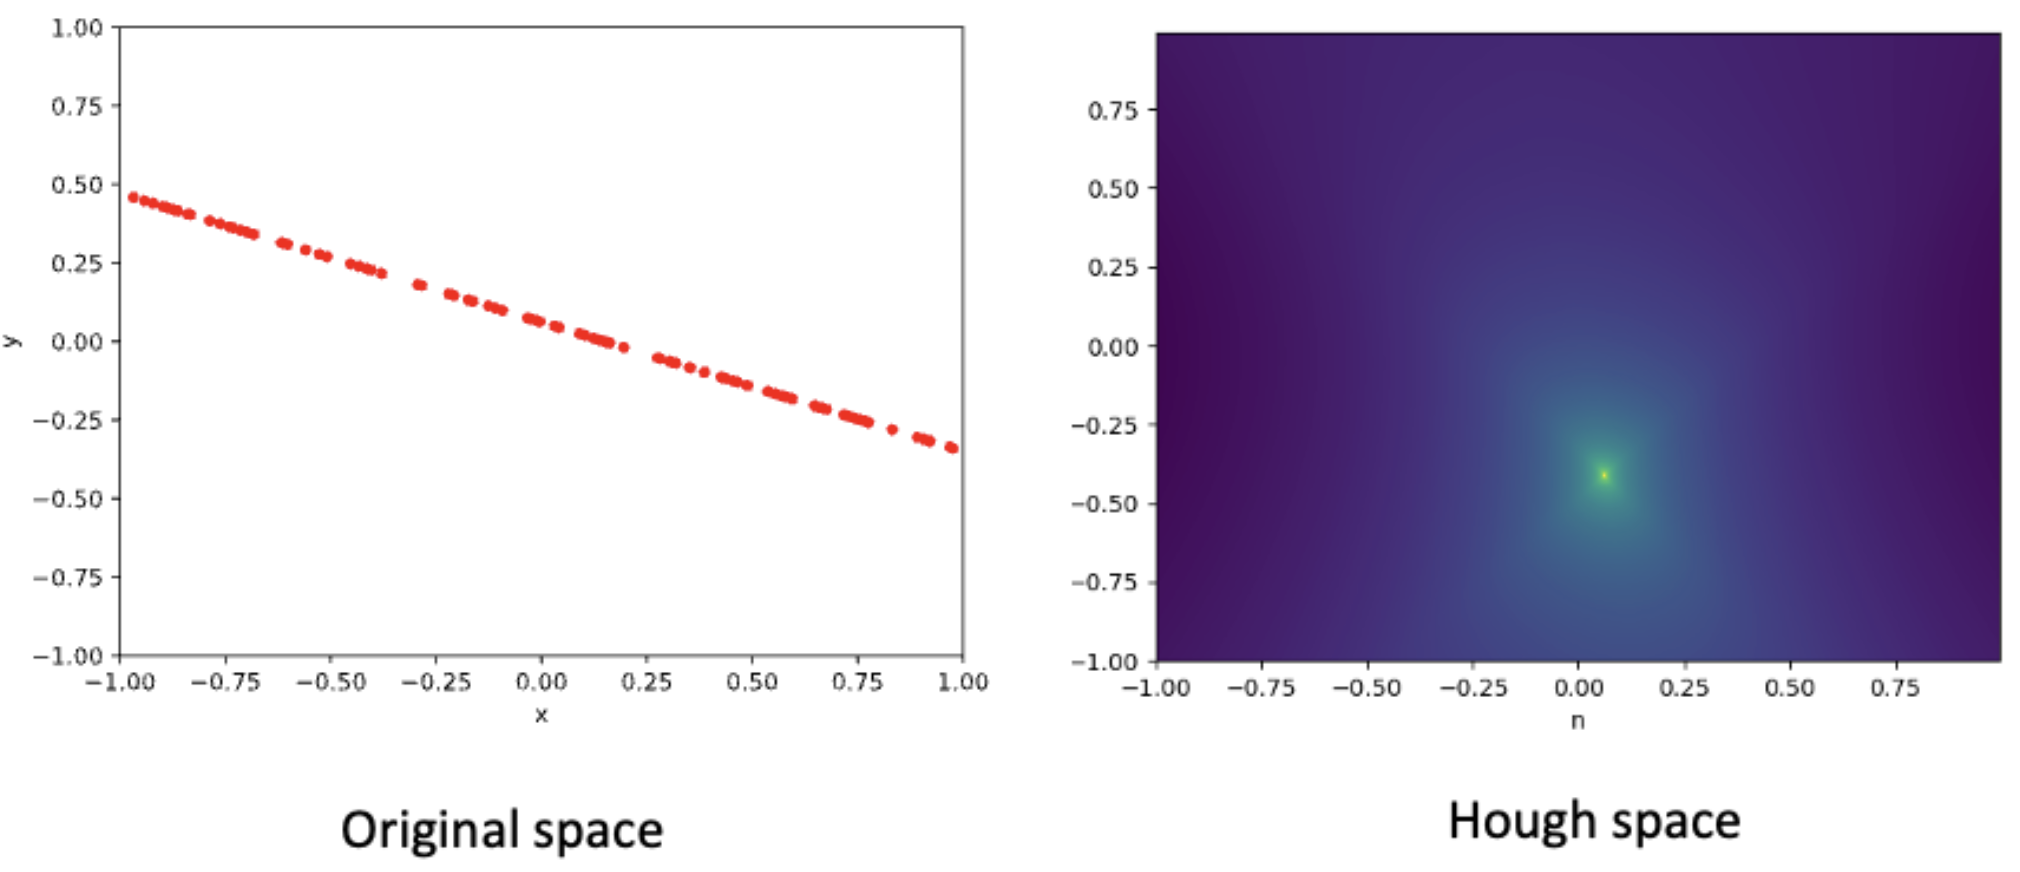
\includegraphics[width=0.8\textwidth]{figures/hough1.png}
    \caption{Hough Transform w/o Noise}
\end{figure}

\begin{figure}[htbp]
    \centering
    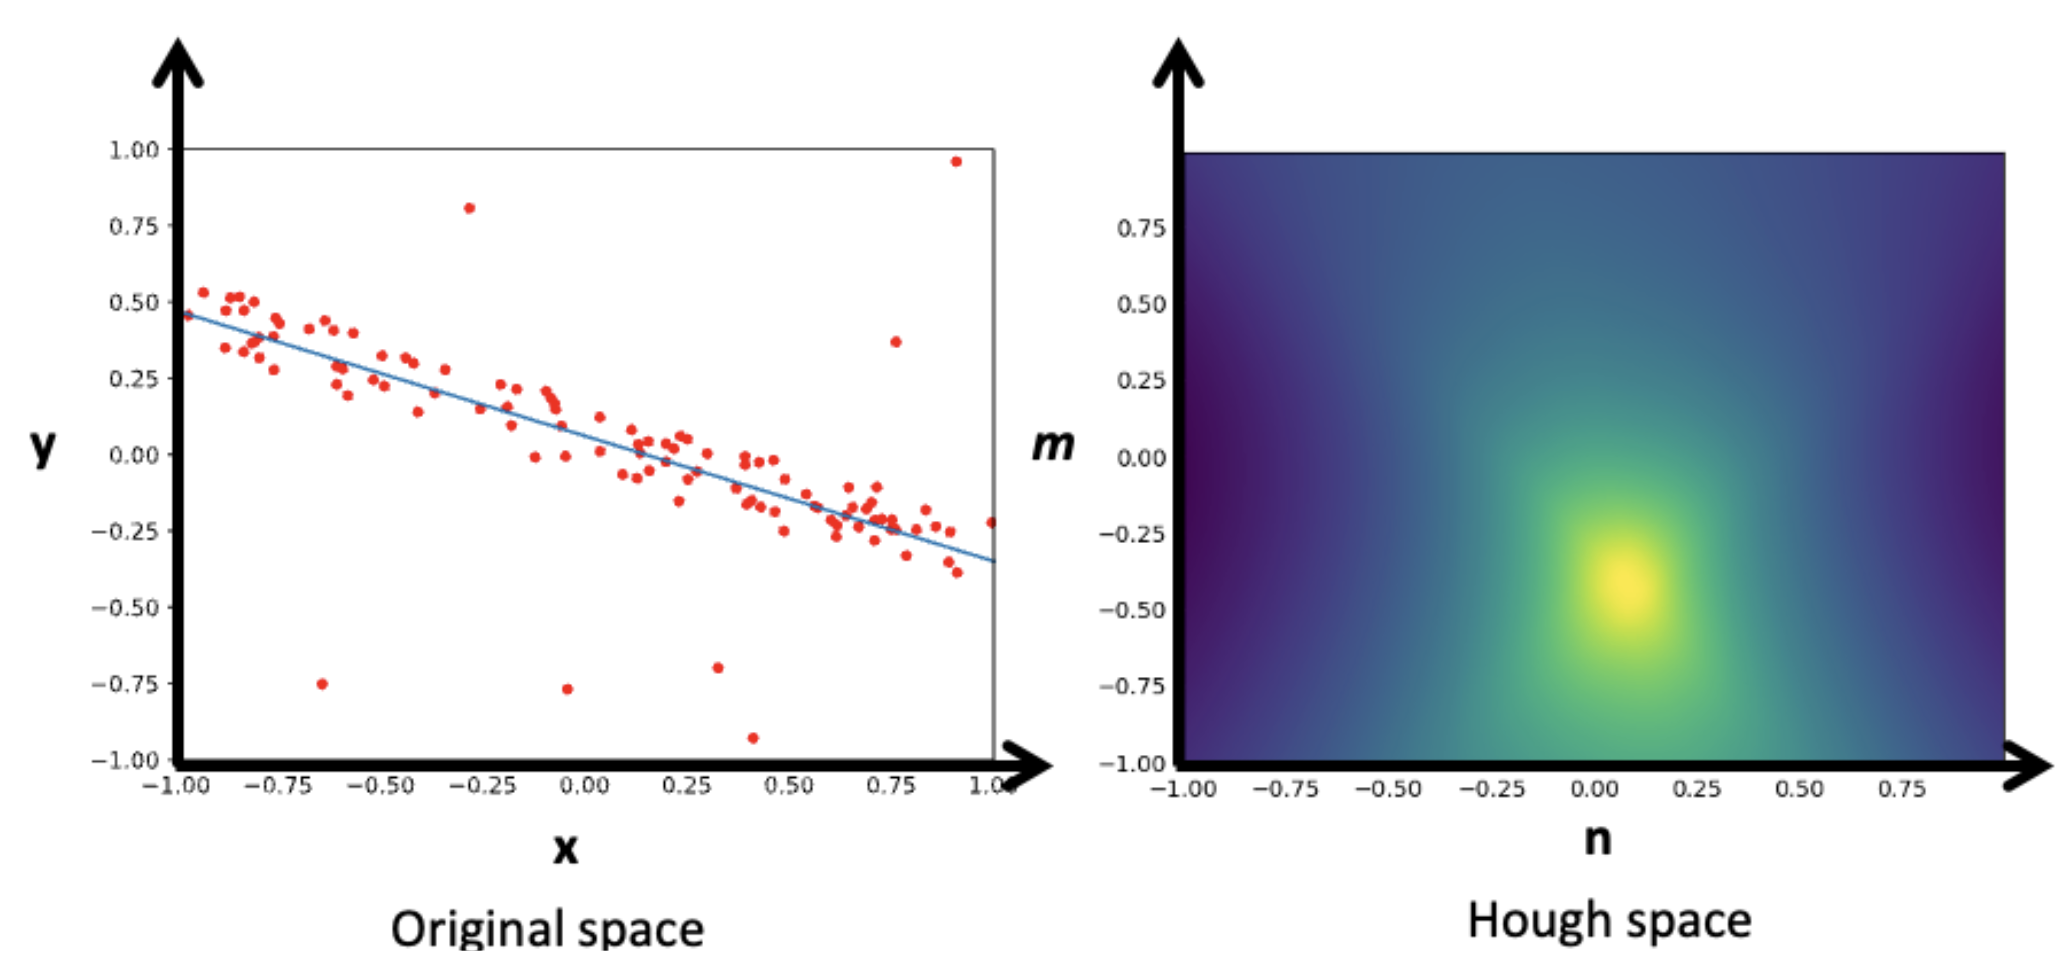
\includegraphics[width=0.8\textwidth]{figures/hough2.png}
    \caption{Hough Transform w/ Noise and Outliers}
\end{figure}
	\chapter{Convolutional Neural Network}

\section{CNN and MaxPooling}

假定输入是$W_1 \times H_1 \times C$的矩阵,可以看作一张图片的宽度,高度,通道数.卷积层需要四个超参数:
filter的数量$K$和大小$F$,步长$S$和零填充参数$P$.经过卷积层后,原本的输入变成$W_2 \times H_2 \times K$,其中

\begin{equation}
	\begin{split}
		W_2 = \frac{W_1 - F + 2P}{S} + 1
		\\
		H_2 = \frac{H_1 - F + 2P}{S} + 1
	\end{split}
\end{equation}

一共需要$F^2CK+K$个参数,其中额外的$K$是每层的bias.

选用卷积核,可以降低feature map的大小.如果直接将图片进行flatten,将会导致大量信息的丢失.

所谓池化操作,就是一种降采样,可以降低图片的大小.比如采用$2\times 2$的大小进行最大值池化,就是将每个$2\times 2$范围内最大的像素的值作为池化后这个像素的取值,
将原来的图片缩减到四分之一大小.池化可以增大感受野.虽然可以通过步长大于一的卷积来代替池化,但是池化不需要参数,更容易优化.

假定输入是$W_1 \times H_1 \times C$的矩阵,则池化层需要两个超参数:大小$F$和步长$S$.池化结果是产生$W_2 \times H_2 \times K$的矩阵,其中

\begin{equation}
	\begin{split}
		W_2 = \frac{W_1 - F}{S} + 1
		\\
		H_2 = \frac{H_1 - F}{S} + 1
	\end{split}
\end{equation}
池化层无需参数.

\section{Summary of CNN-based classification networks}

ConvNets堆叠了卷积层,池化层和全连接层,倾向于使用更小的卷积核和更深的网络结构,尽量避免使用池化层和全连接层 (只使用Conv层).其网络结构大致如下:

\[\texttt{[(Conv-ReLu)*N-Pool?]*M-(FC-ReLu)*K-SoftMax}\]

其中$N$一般不超过5,$M$比较大,$0\le K \le 2$.但最近的网络如ResNet,GoogleNet等也开始突破这些范围.

\section{Pooling Layer affects the paremeter number}

三层 $3\times3$比$7\times7$多了两个relu,非线性性质更好并且参数变少

每 MaxPooling 一次,长宽减半,Channel数量变成两倍

$Param=k^2C^2$,参数变成四倍

$Mem=mnC$,显存变成二分之一

\section{Comparison of MLP and CNN}

如果输入为$W_1 \times H_1 \times C$的矩阵,输出$W_2 \times H_2 \times K$的矩阵,那么FC需要$W_1W_2H_1H_2CK$个参数,一层卷积核大小为$F$的CNN需要$F^2CK$个参数.后者一般比前者小得多.

对于一维情形,$h \in \mathbb R^m, x\in \mathbb R^n$,则$y = h * x$可以被表示为矩阵乘法:

\begin{equation}
	y=h * x=
	\begin{pmatrix}
		h_{1} & 0 & \cdots & 0 & 0 \\
		h_{2} & h_{1} & & \vdots & \vdots \\
		h_{3} & h_{2} & \cdots & 0 & 0 \\
		\vdots & h_{3} & \cdots & h_{1} & 0 \\
		h_{m-1} & \vdots & \ddots & h_{2} & h_{1} \\
		h_{m} & h_{m-1} & & \vdots & h_{2} \\
		0 & h_{m} & \ddots & h_{m-2} & \vdots \\
		0 & 0 & \cdots & h_{m-1} & h_{m-2} \\
		\vdots & \vdots & & h_{m} & h_{m-1}\\
		\vdots &\vdots & \cdots  &0 & h_{m}
	\end{pmatrix}
	\begin{pmatrix}
		x_{1} \\
		x_{2} \\
		x_{3} \\
		\vdots \\
		x_{n}
	\end{pmatrix}
\end{equation}

左侧的矩阵被称为Toeplitz矩阵.由于深度学习当中的卷积参数是学习而来,故不需要像传统的卷积操作一样进行翻转.二维情形的卷积则是一个double block circulant matrix.

由于我们选取较小的卷积核,所以前后层网络之间的连接更为稀疏.而且有更加明显的Parameter Sharing效应,即对每块区域采取相同的参数进行处理.

\textbf{FC和CNN两者哪个表达能力更强呢?}

很显然是FC更强,因为FC的表达范围是CNN的超集.但事实上,使用Conv的结果远好于FC/MLP.那么问题出在哪里呢?

一个显而易见的答案是,FC需要的参数量过于庞大了,一层可能需要上亿甚至更多的参数,这使得其非常难以被优化.另外一个非常重要的原因是,它并没有突出我们在视觉任务中目标的特点,即等变性 (equivariance).

我们知道,在目标分类等任务当中,将图片进行轻微平移,旋转,改变亮度等操作,并不会影响结果.但是,它们都改变了输入的几乎每一个值.
而即使移动了一个像素,FC的输出都将天差地别.换言之,我们要求FC将在它看来输出完全不同的的图像归为一类,这样的矩阵是非常难以寻找的,会在优化过程中产生极大的困难.

那么CNN的表现如何呢?我们先解释上文 equivariance 的含义.其一般定义为:

\begin{equation}
	S_A[\phi(X)] = \phi[T_A(X)]
\end{equation}

这里$A$指代某种操作,而$T_A, S_A$分别代表$X,\phi(X)$空间下的变换.例如将$A$看作左移一像素,忽略边界就有$T[\phi(X)] = \phi[T(X)]$.不变性是等变性在$S_A = I$的特殊情形.

我们需要指出的是,在这里Parameter Sharing就等同于Equivariance to Translation.我们用同样的参数处理每一个局部,那么忽略掉边界后,2D Conv就是等变的.

举个例子,当处理图像的时候,在第一个卷积层进行边的探测是非常有用的,而同样的边或多或少地会出现在图片的其他位置,所以在整个图片范围内进行参数共享是非常可行的操作.
换言之,对于反映同种信息的pixel的识别,在不同位置应该是相同的,这种人类视觉给出的先验知识才是Conv的根本思路.

但需要强调的是,Conv并不是万能的,一个layer作为一个函数,其需要具有何种性质与目标的性质高度相关.我们使用CNN正是因为当前我们的目标具有这种不变性.
但有时你需要位置相关的处理,比如统计一张照片上的绵羊数量,那显然就不能将不同地方的绵羊做相同处理.
这方面的工作就是semi-Conv的工作,发表于CVPR 2018.同样,它也不具有图像缩放,图像旋转等情形下的不变性,需要引入其他机制进行处理.
	\section{CNN Training}

\subsection{Data Preparation}

不仅是在CV当中,在诸如数据科学等学科之中,对数据进行分析之前通常要进行预处理 (processing).
以处理CIFAR-10的$32\times32\times3$数据集,我们有逐通道减去均值 (VGG)或逐通道减去均值然后除以标准差 (ResNet).

标准化有什么作用呢?例如,如果神经元的输入都是正数,那么权重的导数就会都是正的或者负的.而非标准化的数据可能具有很大的数值,
对于权重矩阵的微小变化非常敏感,难以训练.

\subsection{Weight Initialization}

\begin{figure}[htbp]
	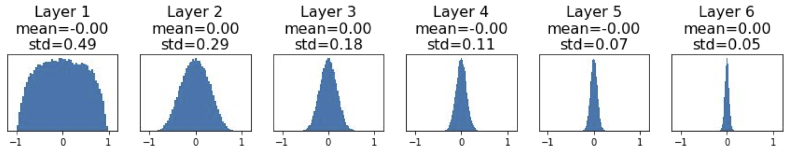
\includegraphics[scale=0.55]{figures/grad_var.png}
	\caption{梯度方差示意图}
	\label{grad_var}
\end{figure}

权重矩阵的初始化并不是一件随意的事情,它代表了我们优化的起点.一个最简单的想法是:用一些小的零均值随机数,
比如调用\texttt{0.01 * np.random.randn (Din, Dout)}生成参数矩阵.但是这样做,由于参数都是一些服从高斯分布的随机数,
这会导致梯度的方差逐层递减,最后梯度非常小,训练困难,如图所示\ref{grad_var}.

一个优化方法是每层都进行标准化,同时令参数的方差为 $\frac{1}{D_{in}}$.

数学推导:

假设 $y=x_1w_1+\cdots+x_nw_n$ ,我们希望 $Var(y)=Var(x_i)$,这样可以保证梯度的方差不会随着层数的增加而变小.那么:

\begin{equation}
	\begin{aligned}
		Var(y) &= Var(x_1w_1+\cdots+x_nw_n)
		\\
		&= Var(x_1w_1)+\cdots+Var (x_nw_n)
		\\
		&= Var(x_1)Var(w_1)+\cdots+Var(x_n)Var(w_n)
		\\
		&= n Var(x)Var(w)
		\\
		\Rightarrow Var(w)=\frac{1}{n}
	\end{aligned}
\end{equation}

在使用ReLu时,可以视为去掉一半神经元,参数方差为 $\sqrt{\frac{2}{D_{in}}}$.

\subsection{Start Optimization}

\begin{figure}[htbp]
	\centering
	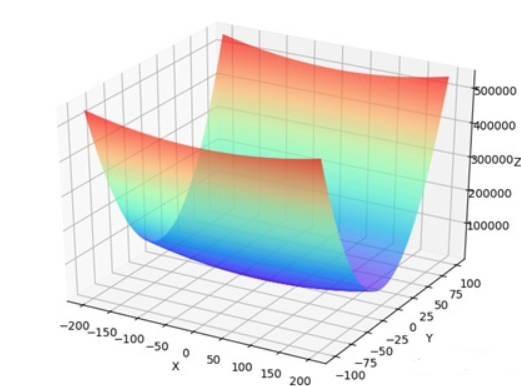
\includegraphics[scale=0.55]{figures/valley.png}
	\caption{山谷示意图}
	\label{valley}
\end{figure}

前面我们提到过用SGD的方法进行训练,但在矩阵的Condition Number\footnote{有关矩阵Condition Number的简单叙述,请见附录.}
较大的时候,SGD的效果仍然不够好.对SGD来说,山谷和鞍点仍然是巨大的麻烦.所谓山谷,
就是类似右图的地形\footnote{本小节的配图和叙述参考了@郑思座的\href{https://zhuanlan.zhihu.com/p/60088231}{这篇文章}.此文还介绍了牛顿动量法和自然梯度法.}:

如果梯度下降进入如图所示的地形,则由于山谷两侧的梯度指向谷底,因此如果山谷中比较平缓,
则很可能在两侧山壁来回打转,或需要很长时间才能到达谷底的最小值.

因此,在SGD的基础上我们可以添加动量方法 (Momentum)\footnote{为什么动量优化work?可以参考这个可视化可交互网站:\href{http://distill.pub/2017/momentum}{Why Momentum Really Works}},
所谓动量方法,就是对历史梯度进行记录,并以一定权重影响当前的梯度.

具体来说,结合物理学上的动量思想,在梯度下降问题中引入动量项$m$和折扣因子$\gamma$,公式变为 

\begin{equation}
	\begin{aligned}
		m &\leftarrow \gamma m+\eta \nabla_{\theta} \mathcal L(\theta)
		\\
		\theta &\leftarrow \theta-m
	\end{aligned}
\end{equation}

其中,$\gamma$表示历史梯度的影响力,$\gamma$越大,历史梯度对现在的影响也越大.
直观上来说,要是当前时刻的梯度与历史梯度方向趋近,这种趋势会在当前时刻加强,否则当前时刻的梯度方向减弱.

我们用SGD+Momentum来对图\ref{valley}进行梯度下降.下面分别是两个不同参数情形时的俯视图.
如果不加momentum,则可以想见点将会以近乎垂直于等高线的方向来回震荡.左图中每个较长的梯度下降之后,
跟着的一段较短并且一定程度矫正了方向,这正是历史梯度的作用.而右图则是$\gamma$较大的情形,
此时历史梯度的权重过大,积重难返,优化效果要差一些.

\begin{figure}[htbp]
	\centering
	\subfigure[$\eta=0.016, \gamma=0.7$]{
		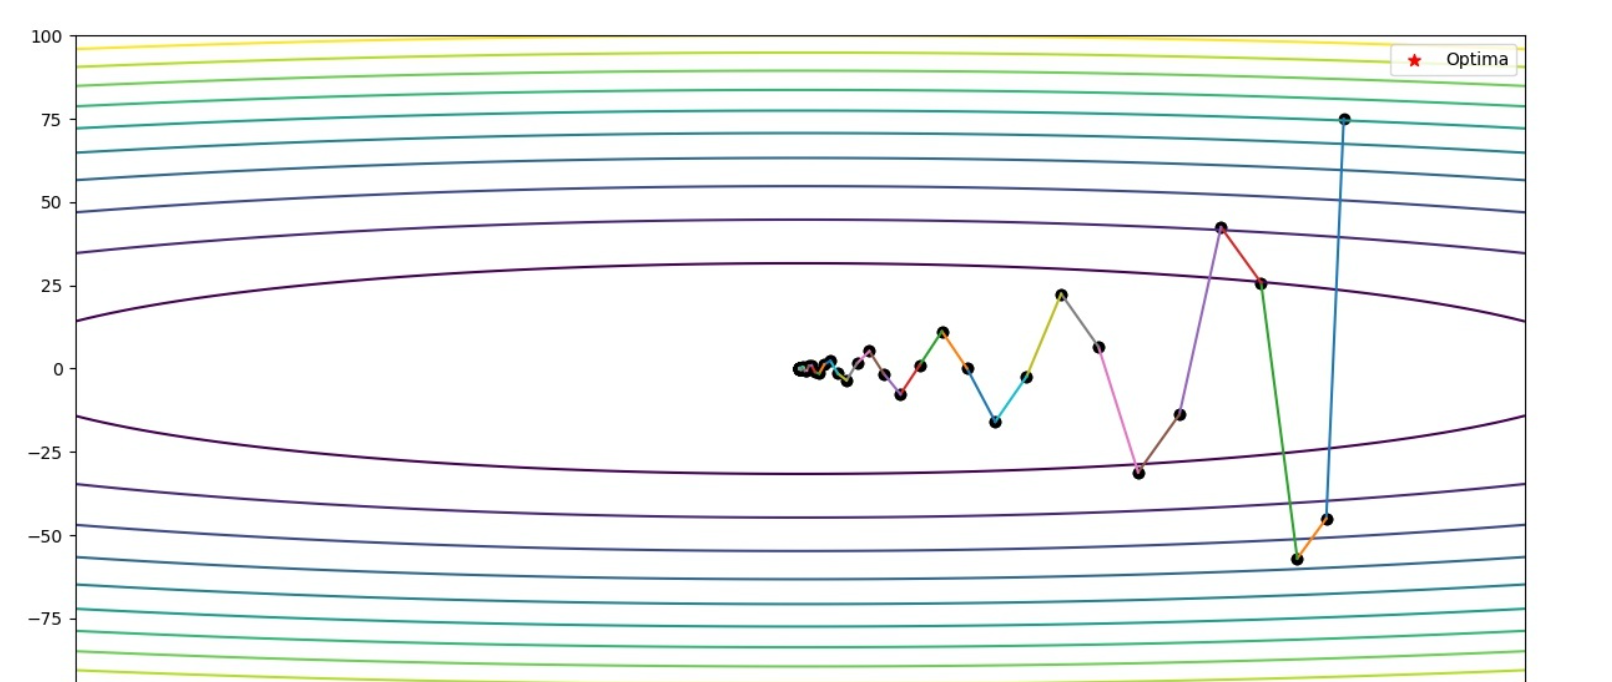
\includegraphics[scale=0.2]{figures/msgd1.png}
	}
	\subfigure[$\eta=0.016, \gamma=0.9$]{
		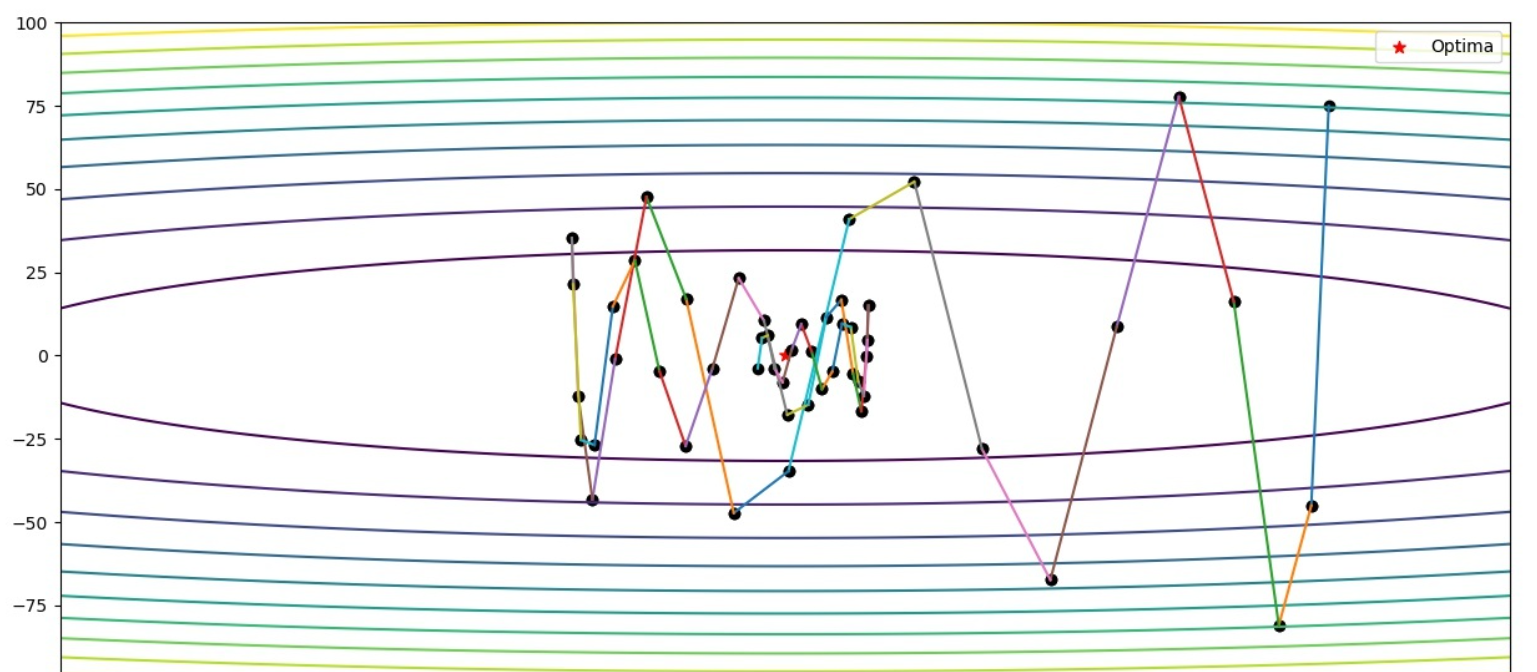
\includegraphics[scale=0.2]{figures/msgd2.png}
	}
\end{figure}

再来考察另一个麻烦:鞍点.存在鞍点意味着此处的 Hessian Matrix 有正负特征值,是不定的,
因而随机梯度下降很可能无法找到下降的方向.
由于深度学习实践中普遍维度较高,比如在1000维当中只有两个维度不是local minimum,
那么SGD也很难跳出这里.这也是偶尔会看到loss长时间不动而突然间骤减的可能原因.

若用$G_{t}$表示第$t$轮迭代的动量,$g_{t}=\eta \nabla_{\theta} \mathcal L(\theta)$
表示第$t$轮迭代的更新量,当$t \rightarrow \infty , G_{\infty}=\frac{g_{0}}{1-\gamma}$,
该式的含义是如果梯度保持不变,最终的更新速度会是梯 度项乘以学习率的$\frac{1}{1-\gamma}$倍.
举例来说,$\gamma=0.9$时,动量算法最终的更新速度是普通梯度下降法 的10倍,意味着在穿越"平原" 
和"平缓山谷"从而摆脱局部最小值时,动量法更有优势.

在书写代码时,我们通常这样写:

\begin{equation}
	\begin{aligned}
		v_{t+1} &\leftarrow \rho v_{t} + \nabla f(x_t)
		\\
		x_{t+1} &\leftarrow x_t - \alpha v_{t+1}
	\end{aligned}
\end{equation}

也就是将velocity项作为梯度的运行时均值.一般取$\rho = 0.9$或$\rho = 0.99$.

Adam就是一种应用了Momentum的优化方法.具体如下图.

\begin{figure}[htbp]
	\centering
	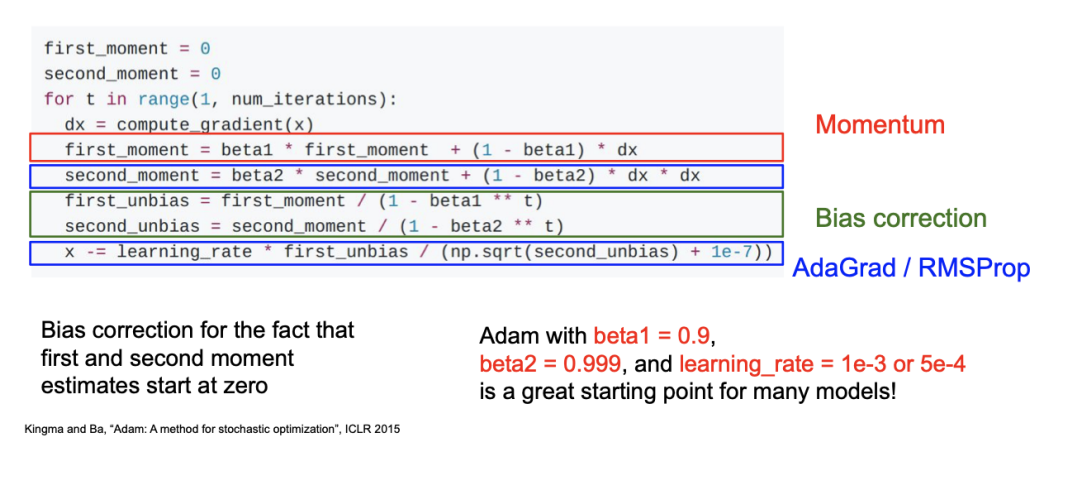
\includegraphics[scale=0.65]{figures/adam.png}
	\caption{Adam}
\end{figure}

\subsection{Learning Rate Schedule}

在神经网络的训练过程中,如何设定学习率的变化策略也是很重要的,因为越靠近最小值,其对学习率的取值可能越敏感,
需要更加精细地取值.我们先来看一张不同大小的学习率对于loss function的影响.
\sout{由此可以看出,好的学习率就应该像临界阻尼一样,让阻尼振荡又快又稳地回到平衡位置...(胡言乱语)}

\begin{figure}[htbp]
	\centering
	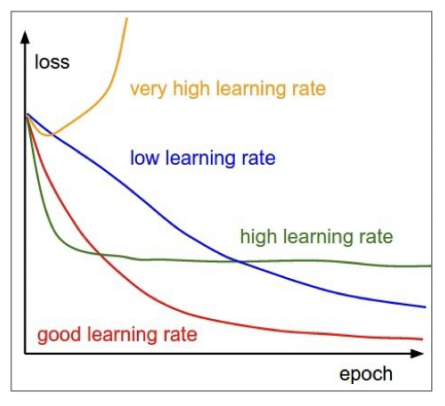
\includegraphics[scale=0.65]{figures/learning_rate_schedule.png}
	\caption{不同学习率对损失函数的影响}
\end{figure}

较低的学习率会使得训练所需时间较长,而过高的学习率会限制最终的结果.如果学习率非常高,可
能loss反而会上升\footnote{这里老师在课上说不一定,并提问:对于 classification 问题,也会上升吗?
有想法的同学欢迎联系笔者,我将在此添加您的真知灼见.
两年之后的笔者对这个问题也没有想法orz}.

一种策略是,在固定轮数之后,缩减学习率.比如ResNet在每30个epoch
\footnote{此处王鹤老师详细解释了iteration和epoch两个概念的区别.一次iteration,
就是跑完一次mini-batch的过程.而epoch的含义则更加灵活.它可指代:1.训练完整个dataset称为一个epoch.
例如将3200张图片分为100个mini-batch,则1 epoch = 100 iteration.  2.每个epoch结束保存一次模型.  
3.epoch作为绘制curve的单元.  4.进行model evalidation的单元.}后将学习率乘以$0.1$.
除此之外还有多种形式,如余弦,线性递减,除以轮数的平方根等.

除了一定轮数之后的递减策略,在训练伊始,也有"热身"的递增策略.过高的初始学习率对优化会产生不利影响,
但在约前5000次迭代中线性增长学习率可以避免这种影响.另外,有一个经验定律:如果将batch的大小增长了$N$,
那么学习率也变为$N$倍.

总之,对于学习率策略而言,Adam+默认学习率在多数情形下都是一个默认较好的选择,甚至它对于常数学习率也常常运行得不错.
而SGD+Momentum的组合可以取得比Adam更好的效果,但恐怕要在学习率策略上花费更多头发.
(余弦函数是个不错的较少参数的策略.)
	\chapter{CNN Training improvement}

\section{Underfitting}

\textbf{\\Batch Normalization}

\begin{wrapfigure}{r}{4cm}%靠文字内容的右侧
	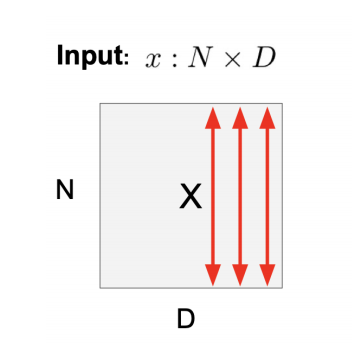
\includegraphics[scale=0.65]{figures/BNsize.png}
	\caption{Input of Batch Normalization}
	\label{Input of Batch Normalization}
\end{wrapfigure}

所谓Batch Normalization,中文译名为"批标准化".其基本操作是在进入激活函数层之前,将数据逐通道进行标准化.
假设输入为$n$个数据,通道数为$D$,如右图.

那么我们需要计算
\begin{equation}
	\begin{split}
		\mu_j &= \frac{1}{N} \sum_{i=1}^{N} x_{i, j}
		\\
		\sigma_j^2 &= \frac{1}{N} (x_{i, j} - \mu_j)^2
		\\
		\hat{x}_{i, j} &= \frac{x_{i, j} - \mu_j}{\sqrt{\sigma_j^2 + \epsilon}}
	\end{split}
	\label{BN calculation}
\end{equation}
其中$\epsilon$是为防止方差为$0$而添加的小量.这一步是标准化的过程,此层还需要进行一步处理:
\begin{equation}
	y_{i, j} = \gamma_{j} \hat{x}_{i,j} + \beta_j
\end{equation}
我们需要学习$\gamma, \beta$这两个$D$维参数.

那么,为什么要进行BN操作呢?

在机器学习领域有个很重要的假设:独立同分布假设,就是假设训练数据和测试数据是满足相同分布的,
这是通过训练数据获得的模型能够在测试集获得好的效果的一个基本保障.那BatchNorm的作用是什么呢?
BatchNorm的作用就是在深度神经网络训练过程中使得每一层神经网络的输入保持相同分布.

对于深度学习这种包含很多隐层的网络结构,在训练过程中,因为各层参数不停在变化,
所以每个隐层都会面临covariate shift的问题,
也就是在训练过程中,隐层的输入分布经常发生变化,这就是所谓的“Internal Covariate Shift”,
Internal指的是深层网络的隐层,是发生在网络内部的事情.

BatchNorm的基本思想就是:能不能让每个隐层节点的激活输入分布固定下来呢?
这样就避免了“Internal Covariate Shift”问题了.

之前的研究表明如果在图像处理中对输入图像进行白化操作的话——所谓白化,就是对输入数据分布进行PCA,
并将各个分量变换到0均值,单位方差的正态分布——那么神经网络会较快收敛.但是白化操作较难进行,而且操作不可导.
而BN可以理解为对深层神经网络每个隐层神经元的激活值做简化版本的白化操作.

BN的基本思想其实相当直观:因为深层神经网络在做非线性变换前的激活输入值随着网络深度加深或者在训练过程中,
其分布逐渐发生偏移或者变动,之所以训练收敛慢,一般是整体分布逐渐往非线性函数的取值区间的上下限两端靠近
(对于Sigmoid函数来说,意味着激活输入值是大的负值或正值),所以这导致反向传播时低层神经网络的梯度消失,
这是训练深层神经网络收敛越来越慢的本质原因,而BN就是通过一定的规范化手段,
把每层神经网络任意神经元这个输入值的分布强行拉回到均值为0方差为1的标准正态分布,
其实就是把越来越偏的分布强制拉回比较标准的分布,这样使得激活输入值落在非线性函数对输入比较敏感的区域,
这样输入的小变化就会导致损失函数较大的变化,意思是这样让梯度变大,避免梯度消失问题产生,
而且梯度变大意味着学习收敛速度快,能大大加快训练速度.

对于每个隐层神经元,把逐渐向非线性函数映射后向取值区间极限饱和区靠拢的输入分布强制拉回到均值为
0方差为1的比较标准的正态分布,使得非线性变换函数的输入值落入对输入比较敏感的区域,以此避免梯度消失问题.

以上关于BN基本思想的叙述来自参考文献\cite{BN}.但是在BN原论文\cite{BNpaper}当中,
作者也提出了只进行 \ref{BN calculation} 的问题:它可能限制模型的表达能力.
以Sigmoid为例,标准化将所有的输入集中于$0$附近,而这里正是Sigmoid的线性近似区域,
这样Sigmoid层的作用就和线性层类似了.因此BN需要再加一项平移和拉伸,并把这两项参数作为学习对象.

总之,BatchNorm的提出试图通过标准化解决深层神经网络当中内部协变量漂移的问题,将数据限制在一定范围内,
并通过平移和拉伸操作减少此操作对模型表达能力的影响.但是,后来有人提出了新的看法:BatchNorm对Internal Covariate Shift
的减缓微乎其微,它是通过平滑化loss landscape来起到作用的.

但BatchNorm有一点需要额外注意:那就是在测试集上运行时,BatchNorm层并不是计算输入的期望方差,
而是调用在训练时储存的$\mu, \sigma$.具体来说,按照以下方式迭代每次运算得到的$\mu_{rms}$:

\begin{equation}
	\begin{cases}
		\mu_{rms}^\prime = \rho \mu_{rms} + (1-\rho) \mu_t 
		\\
		\sigma_{rms}^\prime = \rho \sigma_{rms} + (1-\rho) \sigma_t 
	\end{cases}
\end{equation}

BatchNorm通常位于FC层或Conv层之后,非线性层之前.它有如下的优点:

\begin{enumerate}
	\item 使得深层网络更加容易训练,因为它可以减缓梯度消失.
	\item 允许使用更大的学习率,并且收敛更快.这是因为如果不加BatchNorm,则深层网络容易产生级联效应,
	学习率如果比较大,则前面的layer发生变化将会引起后面的层的剧烈变化,极不稳定.
	\item 网络对于参数的初始化要求降低,因为会进行标准化操作.
	\item 训练的时候使用 BatchNorm 具有正则化的特性:这是因为进行了噪声注入,
	Batchnorm 在每个批次上计算均值和方差,这意味着每个批次的统计特征都会略有不同,
	这种基于小批量的统计计算引入了噪声,类似于数据增强或Dropout的效果.
	这种噪声可以帮助模型避免过拟合,在一定程度上增强了模型的泛化能力.
	\item 测试时不花费开销,可与Conv一同使用
\end{enumerate}

但是同时需要注意:BatchNorm在训练和测试时行为不同!这是Bug的一个常见原因.
此外,一旦使用了BatchNorm,那么Batch就不能太小,否则会使$\mu, \sigma$变得极不稳定,
这可能会导致模型在训练集和测试集上的性能的巨大差异.

\begin{figure}[htbp]
	\centering
	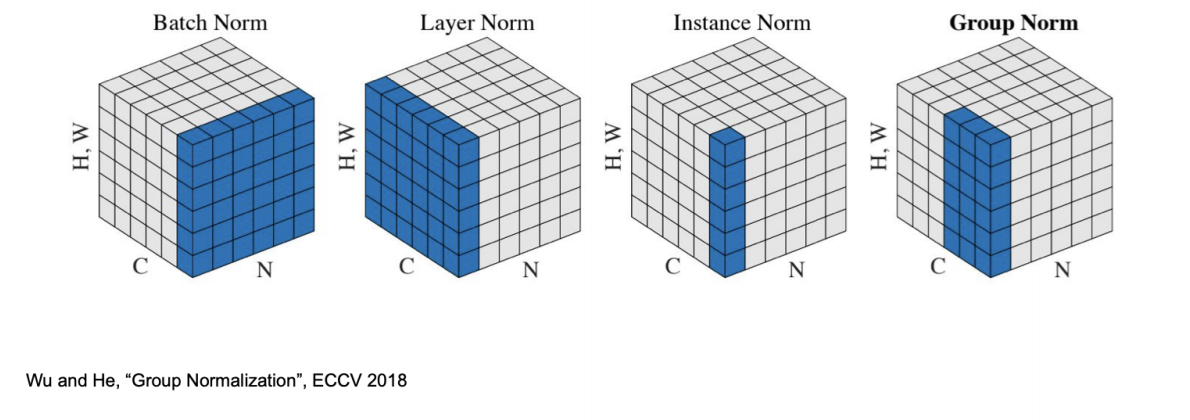
\includegraphics[scale=0.55]{figures/NormalizationTechniques.png}
	\caption{NormalizationTechniques}
	\label{fournorm}
\end{figure}

这样的特性使得人们自然而然提出了一个问题:我们能否绕过BatchSize的限制?如果可行,那么就不会存在训练和测试的差异.

图 \ref{fournorm} 当中的$C,N$分别代表通道数和样本数,$H,W$等维度因为地位相同,被压缩为一个维度,
可以视为图片的宽和高.左一逐通道对所有样本求平均值,正是BatchNorm.要想脱离BatchSize的限制,就必须不沿$N$方向处理.

左二是对$C,H,W$三个维度求平均,这其实蕴含了所有数据服从同一分布的假设,但实际上可能并非如此.
比如,偏绿色的图片在$G$通道上的$\mu$更高,这样做会破坏不同channel的差异性,
效果比BatchNorm更差,因此极少应用于CV领域,但在NLP领域应用广泛.

右二其实就对应了BatchSize=1的情形,其问题前文已述.虽然其存在巨大的不稳定性,
但其$\mu, \sigma$表征了图片风格,因此在Style Transfer当中常用.

右一是由何恺明等人提出的GroupNorm,它将channel分组进行计算,相当于对图2和图3进行了插值.

\begin{figure}[H]
	\centering
	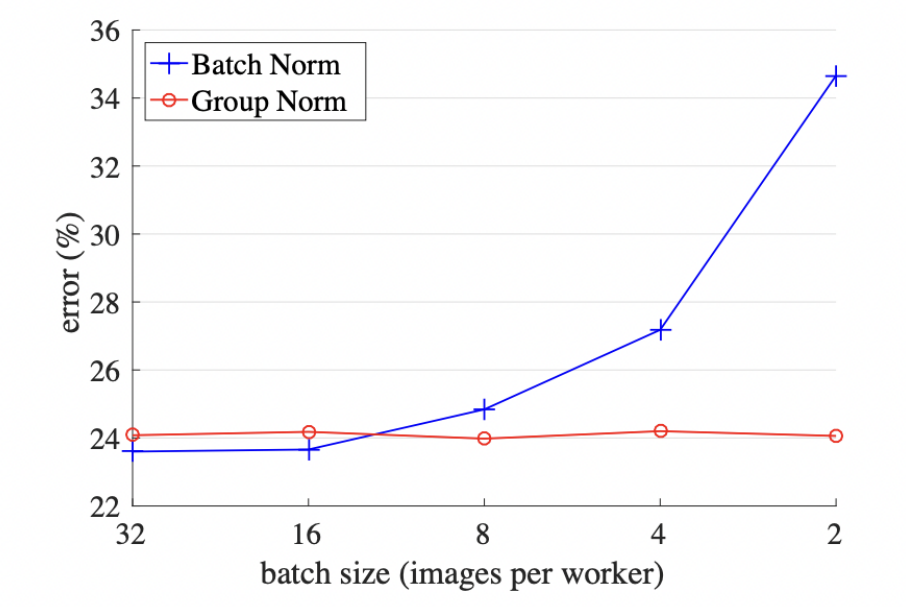
\includegraphics[scale=0.30]{figures/GroupNorm.png}
	\caption{classification error vs batch sizes}
	\label{groupNorm}
\end{figure}

图\ref{groupNorm}是He在论文中给出的一个ResNet-50模型的训练结果,
可以看出在BatchSize较大的时候,BatchNorm表现略优于GroupNorm,
但随着BatchSize减小,前者的错误率快速增长,而后者的错误率则没有明显变化.
当训练集的BatchSize不得不很小或Batch之间差异极大时,应该选用GroupNorm.

\section{Some Questions}

\textbf{问题: 为什么 BatchNorm 不是对 N 上的一维数组进行 norm?}

这是因为会破坏 translation invariance,也就是平移一格变化很大.

\textbf{问题: 后面三个 Norm 需要进行 moving average 吗?}

跟BN不同,后面三个在train和test上都是一样的,没有moving avg mean,因为没有对batch size做norm.

为了防止test的时候batch size过小,BN需要在test的时候使用train的moving avg mean.
而后面三个norm没有这个问题,因为它们不是对batch size做norm的.

\textbf{\\ResNet or Skip Links}

介绍BatchNorm之后,CNN网络结构可修改如下:

\[\texttt{[(Conv-BN-ReLu)*N-Pool?]*M-(FC-BN-ReLu)*K-FC-SoftMax}\]

注意最后的\texttt{FC-SoftMax}之间无需添加\texttt{BN}.那么,层数是越深越好吗?我们来看下图.
\begin{figure}[htbp]
	\centering
	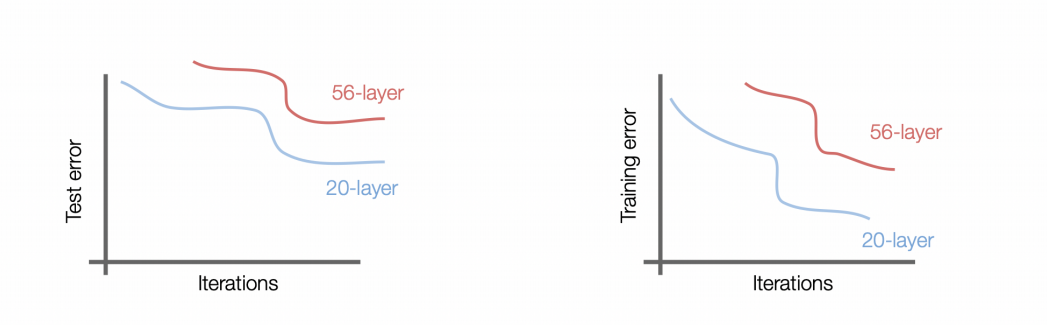
\includegraphics[scale=0.65]{figures/deep-test-err.png}
	\caption{两种深度的神经网络的测试误差(左)和训练误差 (右)}
	\label{过拟合}
\end{figure}

56层神经网络在测试集上误差大于20层,我们可以解释为是过拟合导致,但其在训练集上的误差竟然也更大,
这就说明更深的神经网络表现不佳并不是过拟合导致.那么在CNN变深的过程中,究竟产生了什么问题呢?

现在的事实是:更深的模型具有更强的表达能力 (即更多参数),但是表现却更差.
我们提出一个假设:
可能是因为深层的神经网络更加难以进行优化.这个时候我们应该控制变量找出原因.
\footnote{在接下来将较浅层的输出通过一条旁路直连深层的操作,
老师称之为"寻找一种中间状态",即将浅层网络加上恒等变换层"视为"深层网络,再将两个进行叠加.}
一种让深层网络至少和浅层网络一样好的方法是,将浅层网络加上一些恒等变换的层,"变成"深层网络.
从这种意义上看,更深的网络不应该比浅的差,只要中间的一些层学习成恒等变换即可.这可能预示着,
对于深层网络而言,"恒等"是一个较难学习的特征.这或许是因为深层网络引入太多非线性表达,
在高维的参数空间中难以学习到恒等吧.
\footnote{本小节余下的内容取自\cite{WhyResNetWorks}.}

\begin{wrapfigure}{r}{4cm}
	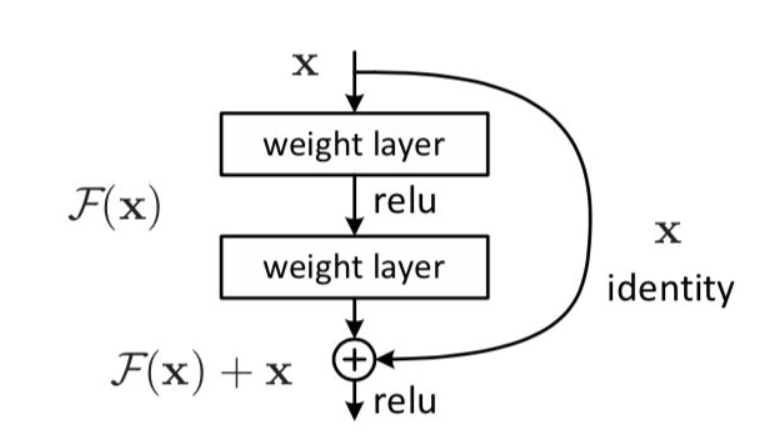
\includegraphics[scale=0.35]{figures/residual_network.png}
	\caption{残差神经网络单元}
\end{wrapfigure}

既然如此,那么一种自然的思路就是:构造天然的恒等.假设神经网络非线性层的输入输出维度一致,那么可以将要拟合的函数分成两个部分:

\begin{equation}
	\mathbf{z}^{(l)}=\mathcal{H}\left(\mathbf{a}^{(l-1)}\right)=\mathbf{a}^{(l-1)}+\mathcal{F}\left(\mathbf{a}^{(l-1)}\right)
	\label{残差神经网络表达式}
\end{equation}

其中 $\mathcal{F}(\cdot)$ 是残差函数.在网络高层,学习一个恒等映射 
$\mathcal{H}\left(\mathbf{a}^{(l-1)}\right) \rightarrow \mathbf{a}^{(l-1)}$ 
即等价于令残差部分趋 近于0,即 $\mathcal{F}\left(\mathbf{a}^{(l-1)}\right) \rightarrow \mathbf{0}$.

残差单元可以以跳层连接的形式实现,即将单元的输入直接与单元输出加在一起,然石再激活.因 
此残差网络可以轻松地用主流的自动微分深度学习框架实现,直接使用BP算法更新参数.

实验表明,残差网络很好地解决了深度神经网络的退化问题,并在ImageNet和CIFAR-10等图像任务上取得了非常好的结果
,同等层数的前提下残差网络也收敛得更快.这使得前馈神经网络可以采用更深的设计.
除此之外,去除个别神经网络层,残差网络的表现不会受到显著影响,这与传统的前馈神经网络大相径庭.

那么,残差神经网络为什么有效呢?

从梯度反向传播的角度,Skip Link提供了一条梯度反向传播的旁路,使得梯度可以更加顺畅地传递到浅层.
我们考虑式\ref{残差神经网络表达式}描述的层,假设残差块不采取任何激活函数,即

\begin{equation}
	\bold{a}^{(l)} = \bold{z}^{(l)}
\end{equation}

考虑$l_1>l_2$两个层,递归地进行展开,有

\begin{equation}
	\mathbf{a}^{\left(l_{2}\right)}=\mathbf{a}^{\left(l_{1}\right)}+\sum_{i=l_{1}}^{l_{2}-1} \mathcal{F}\left(\mathbf{a}^{(i)}\right)
\end{equation}

在前向传播时,输入信号可以从任意低层直接传播到高层.由于包含了一个天然的恒等映射,一定程度上可以解决网络退化问题.
这样,最终的损失函数$\mathcal{L}$对某低层输出的梯度可以展开为

\begin{equation}
	\frac{\partial \mathcal{L}}{\partial \mathbf{a}^{\left(l_{1}\right)}}=\frac{\partial \mathcal{L}}{\partial \mathbf{a}^{\left(l_{2}\right)}}+\frac{\partial \mathcal{L}}{\partial \mathbf{a}^{\left(l_{2}\right)}} \frac{\partial}{\partial \mathbf{a}^{\left(l_{1}\right)}} \sum_{i=l_{1}}^{l_{2}-1} \mathcal{F}\left(\mathbf{a}^{(i)}\right)
\end{equation}

上式说明,反向传播时,错误信号可以不经过任何中间权重矩阵变换直接传播到低层,
一定程度上可以缓解梯度弥散问题(即便中间层矩阵权重很小,梯度也基本不会消失).
综上,可以认为残差连接使得信息前后向传播更加顺畅.

在文章\cite{ResidualNetworksAreExponentialEnsembles}中,
作者提出了另一种观点,认为残差神经网络是由一系列路径集合组装成的模型.

\begin{figure}[htbp]
	\centering
	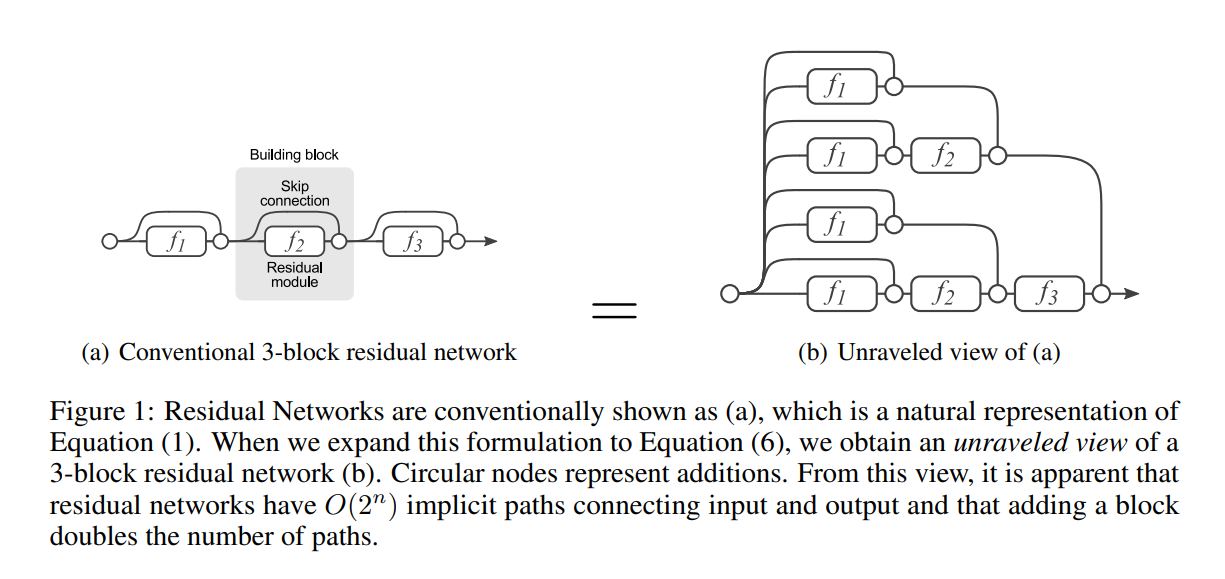
\includegraphics[scale=0.55]{figures/ResNet集成神经网络解释.png}
	\caption{文章给出的配图}
\end{figure}


Andreas Veit等人展开了几组实验,在测试时,删去残差网络的部分网络层
 (即丢弃一部分路径)、或交换某些网络模块的顺序 (改变网络的结构,丢弃一部分路径的同时引入新路径).
实验结果表明,网络的表现与正确网络路径数平滑相关 (在路径变化时,网络表现没有剧烈变化),
这表明残差网络展开后的路径具有一定的独立性和冗余性,使得残差网络表现得像一个集成模型 (ensemble).
作者还通过实验表明,残差网络中主要在训练中贡献了梯度的是那些相对较短的路径.


\section{Overfitting}

过拟合产生的原因是data和model之间的不平等.
例如分类问题,我们给网络输入的数据,对于机器来说就是某个概念的"定义".
但同类事物有共性也有差别,定义应当只取其共性,但神经网络并不一定能做到这一点.
所以,减弱model增强data的手段,有助于打破这种不平衡.

首先我们来看看在神经网络训练过程中常见的generalization gap:
\begin{figure}[htbp]
	\centering
	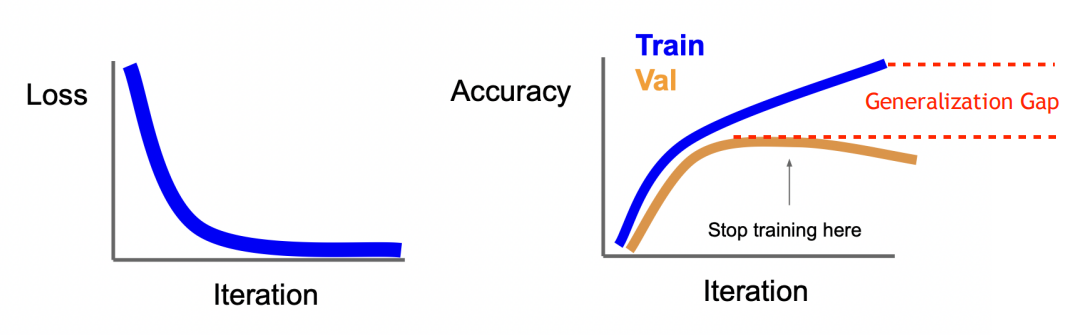
\includegraphics[scale=0.65]{figures/generalgap.png}
	\caption{generalization gap 示意图}
\end{figure}

所谓generalization gap,就是指模型在同分布的训练集和测试集上表现出的准确率差异.
这里右图略有瑕疵,我们说的gap应该是指同一轮测试之后两个集合上表现的差异.
另外需要注意的是:在训练时即使loss一直在减小,也并不说明在测试集上的准确率在提升,
因为可能有过拟合的问题.

对一个过拟合的模型来说,它包含了多于区分数据所必须的数量的参数.为减少过拟合,
我们可以从数据和模型两方面着手处理.数据方面,一种自然的想法是,如果训练集数据充足而且包含较多各种无关特征,
那么模型更不容易过拟合.最简单的方法是增加数据量,但有时这是代价很大的,我们可以对现有的数据进行处理,
获取更多数据.而在模型方面,我们将采取一些限制模型复杂度的处理.
数据方面包括Data Augmentation等,而后者我们会提及正则化与Dropout.

\textbf{\\Data Augmentation}

所谓数据增强 (data augmentation),就是一种利用已有数据人工生成新数据的手段.
常用的手段有翻转 (flip),旋转 (rotation),缩放 (scale),裁剪 (crop),移位 (translation)和
高斯噪声\footnote{当神经网络试图学习可能无用的高频特征(大量出现的模式)时,通常会发生过度拟合.
具有零均值的高斯噪声基本上在所有频率中具有数据点,加入图片中可以有效地扭曲高频特征.
这也意味着较低频率的组件(通常是预期数据)也会失真,但这种困难可以被克服.} (Gaussian Noise)等.

例如,如果我们的网络需要识别猫的图片,那么在训练时,我们可以将一张图片水平翻转,
这当然还是一只猫.于是我们轻松将数据量翻了个倍.

但是!要注意的是,你必须保证\textbf{数据增强之后,你所希望学习的特征并没有发生改变}.
这隐含着一种对称性,\sout{而诺特定理指出每种对称性对应一种守恒量,
我们不难看出数据增强的依赖的对称性对应的守恒量就是标签... (胡言乱语)}
即每一只猫是左右对称的.相对应地,我们很少对猫图片进行上下翻转.
所以,进行正确的数据增强是很重要的.比如下面这种反面教材:

\begin{figure}[htbp]
	\centering
	\subfigure[错误的DA]{
		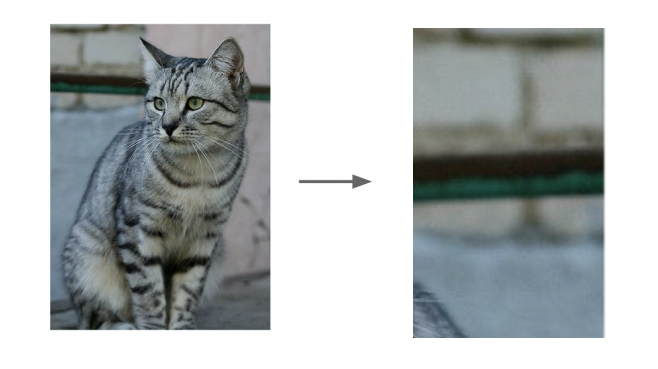
\includegraphics[scale=0.65]{figures/wrongDA.png}
	}
	\subfigure[神经网络直呼我逐渐理解一切]{
		
\includegraphics[scale=0.5]{figures/strangeknowledge.png}
	}
\end{figure}

总之,DA不能太强也不能太弱,很多时候其程度还是需要人工评判.

在空间位置方面的数据增强手段有缩放,裁剪,翻转,填充,旋转,移位,仿射变换 (affine transformation)等.
色彩方面,可以调整亮度 (brightness),对比度 (contrast),饱和度 (saturation),色调 (hue)等.
此外还可以应用GAN/Reinforcement Learning 完成数据增强.

\textbf{\\Regularization}

所谓正则化,就是限制模型复杂度的一种手段.具体做法就是在损失函数当中添加一项正则项:

\begin{equation}
	L(W) = \underbrace{\frac{1}{N}\sum_{i=1}^{N} L_i(f(x_i, W), y_i) }_{Data Loss:\text{模型预测需要拟合训练集}} + \underbrace{\lambda R(W)}_{Regularization:\text{防止模型在训练集上}\textbf{表现太好}}
\end{equation}

举个例子,对于7个散点,我们可以拟合成一条直线,也可以用六次函数经过每一个点,
但后者常常不是我们想要的,而正则项的添加就是对模型训练程度的一个限制.
设想一个模型是六次函数,我们如何限制其表达近似线性的数据?
只需将常数项和一次项系数之外的系数限制在0附近即可.

这种想法与一种哲学原理不谋而合:即Occam's Razar.
我们常用的正则函数有$\mathbb L_2$ Regularization: $R(W) = \sum_{k,l}W_{k, l}^2$,
以及$\mathbb L_1$ Regularization: $R(W) = \sum_{k,l}\abs{W_{k, l}}$,以及其混合等.
使用时需要注意:$\lambda$需要控制正则项的量级,使其与损失函数相当,否则如果正则项过大,
会使得网络全力向简单发展;反之则没有效果.

\textbf{\\Dropout}
简单地说,Dropout就是以某个概率随机使神经元失效.

通常,Dropout 的概率设置在 0.2 到 0.5 之间,表示有 20\% 到 50\% 的概率丢弃一个神经元.
需要注意的是,在训练完成后并应用到推理/测试阶段时,Dropout 是关闭的,此时所有神经元都会被使用.
此外,为了保证神经网络的输出在训练和测试阶段的一致性,在测试阶段需要将所有神经元的输出乘以一个比例
(这个比例等于 Dropout 的保留概率),以补偿训练阶段丢弃的部分 (大小).

在实际使用 Dropout 时,通常是在全连接层和 RNN 层中使用,
尽量避免在卷积层中使用,因为卷积层具有局部特征的结构,随机丢弃会破坏这种局部性.

\textbf{\\BatchNorm作为正则化}

BatchNorm使得进入激活函数的输入必须服从特定的高斯分布,这限制了模型的表达能力,
因此也是一种正则化的手段,有助于减少过拟合.使用BatchNorm后,就不需要再添加Dropout了.

总之,纵观各种正则化的方法,处处透露出 Less is More 的思想,即越简单的表达方式越好.
\footnote{Less is More, but More is different. (笑)}

\section{Summary of Mitigating Overfitting}
原则:平衡数据的多样性和模型的容量.

方法:
\begin{enumerate}
	\item Data Augmentation. (从数据的角度)
	\item BatchNorm. (模型角度)
	\item Regularization. (模型角度)
	\item Dropout. (模型角度)
\end{enumerate}

其中DA和BN用了总是比不用好.后两者视情况而定.Dropout一般只用于较大的FC层.
	\section{Classification}

图片分类是CV领域的核心问题.简单来说,就是给定一张图片,判断其属于何种分类,比如是不是猫或狗等等,这对图片的语义理解非常重要.

但是传统的方法对此类问题难以下手,因为图片通常是由数字的矩阵来描述,而从数字到语义有很大的鸿沟,很难设计某个规则来判定是否属于某类.
比如:对象不同的姿势,不同的摄像机视角,不同的背景信息,不同的光照条件,以及对象被隐藏和类内差异等问题.

对于一个好的图片分类器,应该对上述无关因素不敏感,而这也是data augmentation的意义.比如rotation代表姿势和视角的改变,颜色改变代表光照的变化等.

对于图片分类,我们有下列方法:无参方法有最近邻法,参数方法则可以采用CNN.

\subsection{Nearest Neighbour Classifier}

所谓最近邻,就是将图片视为高维空间的点,将每个训练数据作为已知点,定义一种图片间距离的度量,选取最近的一个 (或几个)
训练数据的类别作为待判断图片的类别.这是一种非常低效的方法,其完美避开了我们上面说到的应具有的标准,对光照/背景/视角/姿势极为敏感,正确率极低,而且需要存储所有训练集.因此,实际中从不使用此种方法.但是最近邻方法在度量学习当中仍有广泛应用.

\subsection{Using CNN for image Classification}

选用CNN之后,我们需要面对的问题有两个:选取何种网络结构,以及如何设计损失函数.
如今分类问题的网络范式是Softmax classifier + cross-entropy loss.
\footnote{对二分类问题,也可采用SVM loss.但是扩展的多分类SVM loss在如今已经极少使用了.}

\subsubsection{SoftMax}

SoftMax就是一个${\mathbb R}^k \to {(0, 1)}^k$的映射.

\begin{equation}
	\sigma(z)_i = \frac{\exp{\beta z_i}}{\sum \exp(\beta z_j)}
\end{equation}

一般取$\beta = 1.$当$\beta \to \infty$时,SoftMax变成Argmax.

所以 SoftMax 是 Soft 的 Argmax.

关于loss的设计,如果正确标签是one-hot的,那么我们可以使用负对数概率(NLL)作为损失函数.
但是如果ground truth也是一个概率分布(有时这是人为的),
那么我们就需要对两个概率分布的距离度量给出定义.在信息论领域常用的度量是KL divergence $D(P \parallel Q)$,其定义如下:

\begin{equation}
	D(P \parallel Q) = \sum_{x \in \mathcal X} P(x) \log \frac{P(x)}{Q(x)}.
\end{equation}

这个度量并不满足距离的定义,因为其满足正定性,而不满足对称性和三角不等式.

我们不难看出
\begin{equation}
	D(P \parallel Q) = \underbrace{-\sum_{x \in \mathcal X} P(x)\log Q(x)}_{H(P, Q)} - \underbrace{\xk{-\sum_{x \in \mathcal X} P(x) \log P(x)}}_{H(P)}.
\end{equation}
即KL divergence是相对熵和分布$P$的熵之差.如果$P$是groud truth的分布,那么第二项成为常数,就得到了我们的交叉熵损失函数:
\begin{equation}
	\mathcal L_{CE} = H(P, Q) = -\sum_{x \in \mathcal X} P(x) \log Q(x).
\end{equation}

交叉熵函数在随机初始化时,取值约为$\log (\text{sum of classes})$.它没有上界,有下界$0$.

所以 CrossEntrophyLoss 应该在 $\log{\text{类别数}}$ 开始下降

\subsection{Cross Entrophy Loss V.S. Accuracy}

1.CEL有可能已经降到了log2,acc仍是0.例子:$\Pr=[0.499,0.501]$,仍然输出错误答案,但是 $loss=\log2$ 很小

2.$acc=100\%$的时候,CEL仍然可能是初始化的 $\log(N)$ , 同理举一个例子:$\Pr=[0.498,0.001,0.001]$

综上所述,两者没有确定关系,训练一定要同时画两个曲线
	\chapter{CNNs for Image Classification}

当我们分析一个CNN的结构时,需要考虑以下的方面:

\begin{enumerate}
	\item 表示能力
	\item 是否适合任务
	\item 是否容易优化
	\item 代价
\end{enumerate}

\section{Reception Field}

如图,使用三层3*3卷积层,感受野与一层7*7卷积层相同.

\begin{figure}[htbp]
	\centering
	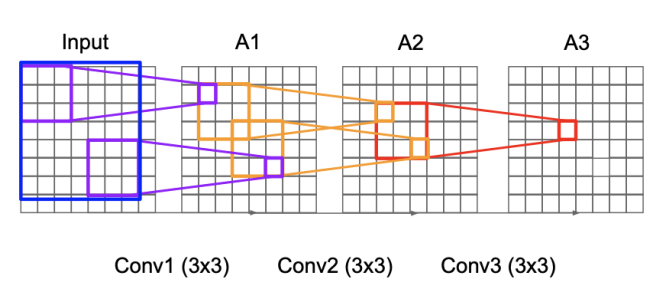
\includegraphics[scale=0.85]{figures/receptivefield.png}
	\caption{三层3*3卷积核的感受野}
\end{figure}

感受野是一个很重要的概念,它表征一个数据可以接收到原图多大范围的信息.
我们这里姑且认为感受野相同则表达能力相同.我们希望可以在神经网络的中部将整个图片纳入感受野,
这样在后面可以进行全图的pixel信息的交流,有利于结合多个特征.例如:结合狗的耳朵和毛色进行判断.

既然三层3*3卷积层,感受野与一层7*7卷积层相同,那么为什么要选用小而深的网络呢?
其一,层数增加,网络的非线性性增加,分割能力更强.此外,参数量也更小 ($3\times 3^2 C^2 < 7^2C^2$).
	\section{Segmentation}

当图片出现不同的对象(例如同时出现猫狗),那么能否将属于同类的pixel分到一起?Not a global label.

Image segmentation:将图片分割为连贯的各个对象,不关心其语义.经典方法:grouping and clustering.
后者就是指将相似的数据点分为一组,然后给予它们一个标识符.

clustering-based segmentation:对于实际图片,颜色当然不可能如此理想.
因此我们要选取三个"中心"来代表,然后将每个pixel以离其最近的中心作为标记.

目标函数:
\begin{equation}
	c^*, \delta^* = \arg \min_{c, \delta} \frac{1}{N} \sum_{j}^{N} \sum_{i}^{k} \delta_{ij} (c_i - x_j)^2.
\end{equation}

很难求解.

很多时候,这个问题是一个"先有鸡还是先有蛋"的问题.即何者优先?

破解之法:如果我们提前知道有$k$个center,则可以调用kmeans.实际就是random initialization.

coordinate decent是一个启发式策略(先找一个方向的最小值,然后下降).但无论如何,kmeans对于初始化非常敏感.它必须提前知道几个group,
并且是无监督的.kmeans实际上进行了对intensity进行了quantum.除此之外还有mean shift.\footnote{其实没人会拿intensity做kmeans.
因为intensity显然不能体现pixel的相关性.}

总结:grouping-based:只关心局部,不关心语义,不可能达到high-level.是bottom-up的方法.而神经网络则是top-down的.

由于纯粹的Instance segmentation已经极为少见,因此今天提及这个词,多是带语义的.

我们今天的问题:Semantic segmentation.实际上就是对每个pixel进行classification.

segmentation时候的一大问题:对每个patch,分类极度依赖上下文.(纯黑的牛)因此,将每个pixel割裂开是不可能实现分类的.

原先的神经网络:图像->padding/strided cnn->拉成vector->MLP->softmax->类别信息.
这是一个不断提取特征的过程.但在segmentation当中,
我们的输出应该与输入一样大.怎么把feature map先变小再变大?
我们的想法是:先缩小提取特征(两头牛),然后回到原图上以此为原则,寻找.

\begin{wrapfigure}{r}{4cm}
	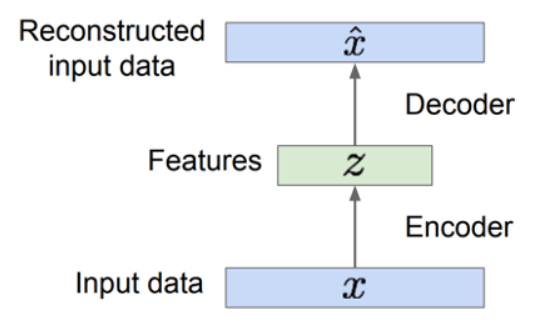
\includegraphics[scale=0.5]{figures/autoencoder.png}
	\caption{name of the figure}
\end{wrapfigure}
NN核心概念:Auto-Encoder.自监督.定义reconstruction loss
\begin{equation}
	\tnorm{\bm x - \hat{\bm{x}} }
\end{equation}

Encoder MLP $f:\mathbb R^m \to \mathbb R^h, h \ll m$.decoder:$g:\mathbb R^h \to \mathbb R^m$.
对于$H \times W \times 3$的图像,实际维度到不了这么多.因此可以进行encode.

考虑classification:$\mathbb R^{H \times W \times 3} \to \{0, 1\}^{k}$.
这样我们就用一个词表示了原图.同样,对于Auto-Encoder,
也是如此,即我不相信这么多像素都是独立分布,
应该是$H \times W \times 3$空间的低维曲面.
同样对于segmentation,我们希望从原图到特征map,然后回到原图,获得分类,而不需要原图的RGB信息.

In-Network Unsamping:Unpooling.

第一种是copy-paste,需要用conv对raw unsamping image进行处理.

In-Network Unsamping:Max Unpooling:记住哪个位置是池化中最大的.
也就是说,并不是所有信息都在bottle neck(中间小的部分)处.这也需要进行大量conv加工.

能不能在一步之内完成?Learnable unsampling:Transpose convolution.
学习出来一个conv,从$2 \times 2 \to 4 \times 4$.Fully Convolutional Network.
全都是Conv进行降采样和升采样.

每一次把feature map变小,后面层的conv的reception field都会变大,
比不做dimentional reduce的图片感受野更大.
有助于提取global context.bottleneck的双重意义:增大感受野,减小size.

关键:增大感受野,收缩image从而集中特征,去除无用.

\begin{wrapfigure}{r}{6cm}
	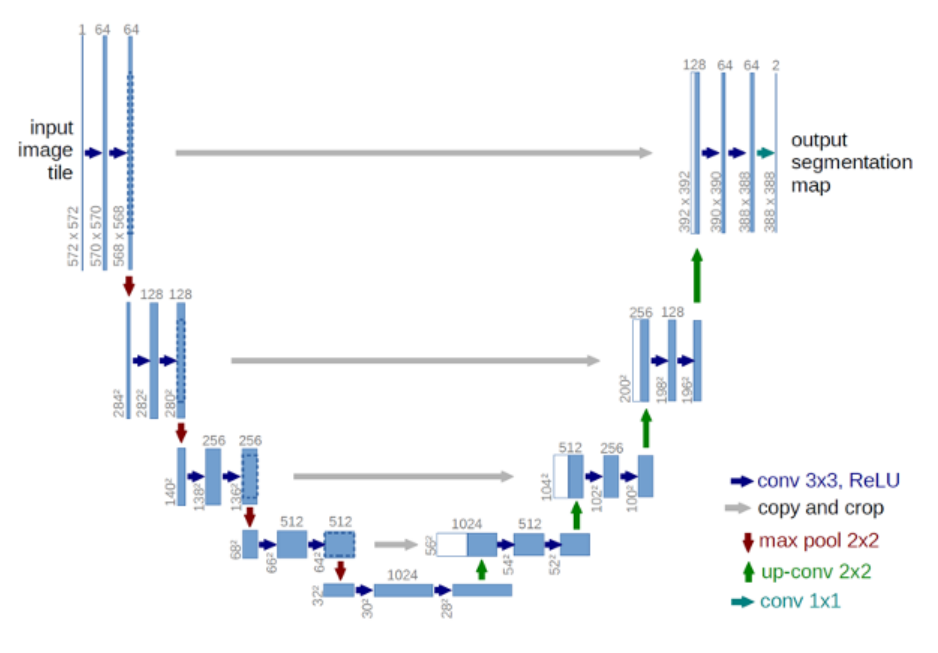
\includegraphics[scale=0.4]{figures/UNetstructure.png}
	\caption{UNet的结构示意图}
\end{wrapfigure}

那么FCN有什么问题呢?我们先来看看它的bottle neck存储了什么?降低resolution,多个channel.
现在在neck里面的内容本来就不多,你还要求通过相同的升采样之后,还能还原出boundary,
这件事与classification相比,不是一句话能说完的,neck里恐怕很难同时存储下特征和原图的boundary信息.


那么我们让各个层次的resolution经过几层conv\footnote{前几层可以理解为在寻找corner和edge.}
直接连接到对称的升维操作,照着把bound画出来就可以,中间neck就只需要记context了.
这是一个非常经典的结构,被称为UNet,也是如今Segmentation乃至depth detection,
dense prediction都需要参考的结构,甚至也是Diffusion model\footnote{但是非常有趣的是U-net最初是在生物学语义分割中提出的.2024笔者注}的一个重要的 Backbone.


Evaluation Metrics: Pixel Accuracy.

\begin{equation}
	\text{accuracy} = \frac{TP+TN}{TP+TN+FP+FN}
\end{equation}

当然这很有问题:比如一个人头只占据整个图片,那么将整个图片预测为背景,那么错误率也很低,但是这很显然不对.

另一个loss:IoU->mean of every class IoU -> soft IoU.
	\section{3D Vision}

Computer vision deals with:acquiring,processing,analyzing,and understanding,(might also include) 
generating or imagining visual data.

联系深度图,RGB图和点云的概念------ camera.RGB可以视作光打到深度图上,对RGB进行采样得到.

如何设计camera?多个光源照在一点,会产生blurring.因此产生了Pinhole camera.我们可以简单地描述其几何关系:
\begin{figure}[htbp]
	\centering
	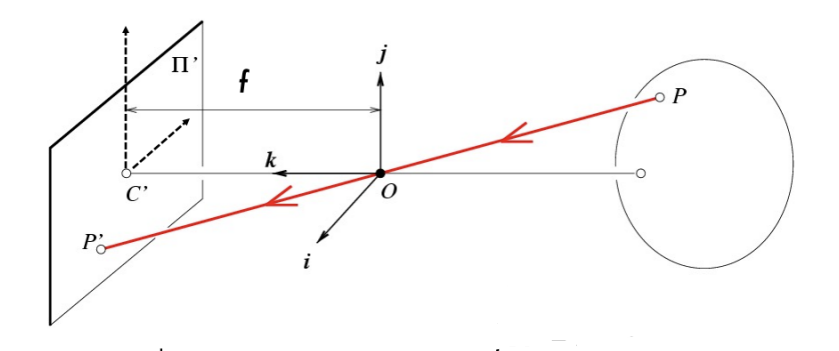
\includegraphics[scale=0.65]{figures/pinholecamera.png}
	\caption{pinhole camera的几何关系}
\end{figure}

满足如下变换
\begin{equation}
	\begin{cases}
		x^\prime &= f\disp\frac{x}{z}
		\\
		y^\prime &= f\disp\frac{y}{z}
	\end{cases}
\end{equation}

aperture size 实际上控制模糊程度和亮度.所以我们可以添加透镜 (lens),透镜可能产生畸变,因此真实相机往往复杂得多.

\subsection{Intrinsics}

上述变换的本质是一个映射$E: \mathbb{R}^3 \to \mathbb R^2$.投影操作,projection mapping.我们还需要完成两件事:
从实际的度量 (米)转换到pixel为单位,以及在图片中,左下角为零点,而非中心,因此需要添加offset.

\begin{equation}
	P=(x, y, z) \rightarrow P^{\prime}=\left(\alpha \frac{x}{z}+c_{x}, \beta \frac{y}{z}+c_{y}\right)
\end{equation}

能否用矩阵表示?很遗憾,这不是线性变换.因此引入homogeneous coordinate system,即增加一个维度作为除法.

\begin{equation}
	P_{h}^{\prime}=\left[\begin{array}{c}
		\alpha x+c_{x} z \\
		\beta y+c_{y} z \\
		z
	\end{array}\right]=\left[\begin{array}{cccc}
		\alpha & 0 & c_{x} & 0 \\
		0 & \beta & c_{y} & 0 \\
		0 & 0 & 1 & 0
	\end{array}\right]\left[\begin{array}{l}
		x \\
		y \\
		z \\
		1
	\end{array}\right]
\end{equation}

如果考虑相机坐标的screw,如下图,则需要进行简单的变换:
\begin{equation}
	\begin{cases}
		x &= \alpha(\hat x - \cot \theta \hat y) + c_x
		\\
		y &= \beta \disp\frac{\hat{y}}{\sin \theta} + c_y
	\end{cases}
\end{equation}

\begin{figure}[htbp]
	\centering
	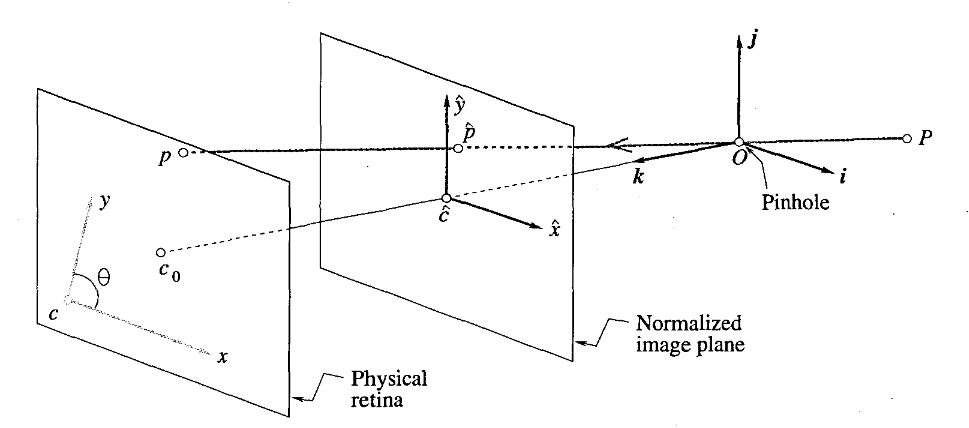
\includegraphics[scale=0.65]{figures/image_plane.png}
	\caption{成像过程坐标示意图}
\end{figure}

最后得到

\begin{equation}
	P^{\prime}=\left[\begin{array}{cccc}
		\alpha & -\alpha \cot \theta & c_{x} & 0 \\
		0 & \frac{\beta}{\sin \theta} & c_{y} & 0 \\
		0 & 0 & 1 & 0
	\end{array}\right]\left[\begin{array}{l}
		x \\
		y \\
		z \\
		1
	\end{array}\right]
\end{equation}

进行分解后表示为
\begin{equation}
	P^\prime = \bd M P = \bd K \begin{bmatrix}
		\bd I & \bd 0
	\end{bmatrix} P
\end{equation}

其中,矩阵$\bd K$定义为
\begin{equation}
	\bd K = \begin{bmatrix}
		\alpha & -\alpha \cot \theta & c_x
		\\
		0 & \frac{\beta}{\sin \theta} & c_y
		\\
		0 & 0 & 1
	\end{bmatrix}
\end{equation}

它是相机的内部参数,拥有$\alpha, \beta, \theta, c_x, c_y$五个自由度.

\subsection{Extinsics}
上一节当中,我们从camera coordina system->retina plane metric->image coordinate system.
但是我们希望完成从world coordinate到image coordinate system的转变.不难看出,
这是两个空间直角坐标系的平移和旋转变换.首先我们来看平移:

对于点$P$,如果要将其平移向量$\bm T$,则可以用如下的矩阵乘法表示:
\begin{equation}
	P^{\prime} \rightarrow\left[\begin{array}{ll}
		\mathbf{I} & \bm T \\
		\bm 0^\top & 1
	\end{array}\right]_{4 \times 4}\left[\begin{array}{c}
		x \\
		y \\
		z \\
		1
	\end{array}\right]
\end{equation}

对于旋转,我们先考虑平面直角坐标系的情形.假如最开始的坐标系为$S$,而$S^\prime$是将$S$逆时针旋转$\theta$,
那么可以得出如果要将$S$中的向量逆时针旋转$\theta$就是将坐标乘以$R_\theta$,其中
\begin{equation}
	R_{\theta} = \begin{bmatrix}
		\cos \theta & - \sin \theta
		\\
		\sin\theta & \cos \theta
	\end{bmatrix}
\end{equation}

原理即是将所有基底旋转$\theta$,坐标表示不变,则自然就随基底旋转.同样对于两个坐标系,$O\bm i \bm j \bm k$
和$O \bm i^\prime \bm j^\prime \bm k^\prime$,将前者坐标下的点$(x, y, z)$的基底向后者旋转,则需要左乘

\begin{equation}
	\bd R = \begin{bmatrix}
		\bm i^\prime \cdot \bm i  & \bm j^\prime \cdot \bm i & \bm k^\prime \cdot \bm i
		\\
		\bm i^\prime \cdot \bm j  & \bm j^\prime \cdot \bm j & \bm k^\prime \cdot \bm j
		\\
		\bm i^\prime \cdot \bm k  & \bm j^\prime \cdot \bm k & \bm k^\prime \cdot \bm k
	\end{bmatrix}
\end{equation}

但是,如果我们想在后者的坐标系中表示同一个向量(注意这两者的区别),那就需要左乘此矩阵的逆.由于此矩阵正交,所以也就是左乘其转置.

可以结合二维情形验证上述表达式.除此之外,我们还可以将旋转分解为三个方向的旋转:

\begin{equation}
	\begin{aligned}
		R_{x}(\alpha) &=\left[\begin{array}{ccc}
			1 & 0 & 0 \\
			0 & \cos \alpha & -\sin \alpha \\
			0 & \sin \alpha & \cos \alpha
		\end{array}\right],
		R_{y}(\beta) =\left[\begin{array}{ccc}
			\cos \beta & 0 & \sin \beta \\
			0 & 1 & 0 \\
			-\sin \beta & 0 & \cos \beta
		\end{array}\right],
		R_{z}(\gamma)= {\left[\begin{array}{lll}
				\cos \gamma & -\sin \gamma & 0 \\
				\sin \gamma & \cos \gamma & 0 \\
				0 & 0 & 1
			\end{array}\right] }
	\end{aligned}
\end{equation}

\begin{equation}
	P^{\prime} \rightarrow\left[\begin{array}{ll}
		\bd R & \bd 0 \\
		\bd 0^\top & 1
	\end{array}\right]_{4 \times 4}\left[\begin{array}{c}
		x \\
		y \\
		z \\
		1
	\end{array}\right]
\end{equation}

将平移和旋转结合,我们就有了统一的形式:

\begin{equation}
	P^{\prime}=K\left[\begin{array}{ll}
		I & 0
	\end{array}\right] P=K\left[\begin{array}{ll}
		I & 0
	\end{array}\right]\left[\begin{array}{ll}
		R & T \\
		0 & 1
	\end{array}\right]_{4 \times 4} P_{w}=K\left[\begin{array}{ll}
		R & T
	\end{array}\right] P_{w}
\end{equation}

其过程示意图如下:

\begin{figure}[htbp]
	\centering
	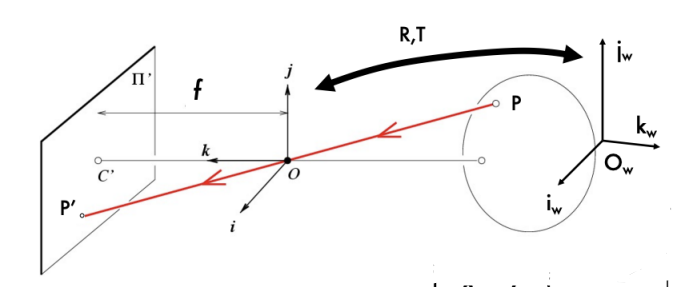
\includegraphics[scale=0.75]{figures/transform_all.png}
	\caption{坐标变换的全过程}
\end{figure}

若令$M = \bd K[\bd R \ \ \bd T]$,设其三个行向量为$\bm m_1, \bm m_2, \bm m_3$,则有
\begin{equation}
	P^\prime = \left(\frac{\bm{m}_{1} \bm P_{w}}{\bm{m}_{3} \bm P_{w}}, \frac{\bm{m}_{2} \bm P_{w}}{\bm{m}_{3} \bm P_{w}}\right)
\end{equation}

投影变换的性质:点映射成点,线映射成线,近大远小.

\subsection{weak perspective}

在弱透视模型中,点首先用正交投影投影到参考平面,然后用射影变换投影到图像平面.如下图:

\begin{figure}[htbp]
	\centering
	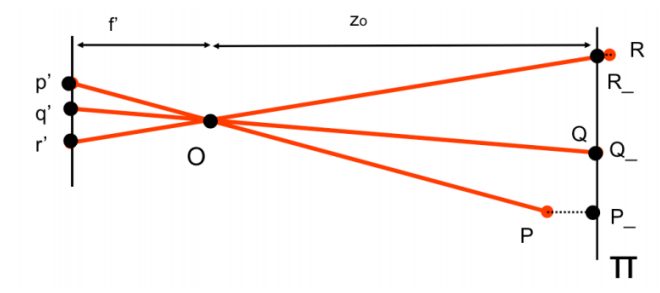
\includegraphics[scale=0.8]{figures/weak_perspective.png}
	\caption{weak perspective}
\end{figure}

这里的正交投影可以表示为

\begin{equation}
	\bd O = \begin{bmatrix}
		1 & 0 & 0 & 0
		\\
		0 & 1 & 0 & 0
		\\
		0 & 0 & 0 & z_0
		\\
		0 & 0 & 0 & 1
	\end{bmatrix} \xlongequal{\text{def}} 
	\begin{bmatrix}
		\bd O^\prime & \bm z_0
		\\
		\bm 0^\top & 1
	\end{bmatrix}
\end{equation}
即将所有$z$分量变为$z_0$.随后根据我们的变换公式
\begin{equation}
	\bm P^\prime = \bd K \begin{bmatrix}
		\bd I & \bm 0
	\end{bmatrix} \bd O 
	\begin{bmatrix}
		\bd R & \bd T
		\\
		\bm 0^\top & 1
	\end{bmatrix}
	\bm P
	= \bd K_{3\times 3} 
	\begin{bmatrix}
		\bd O^\prime \bd R & \bd O^\prime \bd T + \bm z_0
	\end{bmatrix}_{3\times 4} 
	\bm P_{4\times 1} 
\end{equation}

进一步,由于$\bd O^\prime$的第三行全零,因此中间矩阵的第三行是$[0, 0, 0, z_0]$.
记$\bd R_2, \bm t_2$分别是$\bd R, \bd T$的前两行,上式可以改写为

\begin{equation}
	\bm P^\prime = \bd K 
	\begin{bmatrix}
		\bd R_2 & \bm t_2
		\\
		\bm 0^\top & z_0
	\end{bmatrix}
	\bm P
\end{equation}

我们记
\begin{equation}
	\bd K = 
	\begin{bmatrix}
		\bd K_2 & \bm p_0
		\\
		\bm 0^\top & 1
	\end{bmatrix}, \quad 
	\bd K_2 = 
	\begin{bmatrix}
		\alpha & -\alpha \cot \theta
		\\
		0 & \frac{\beta}{\sin \theta}
	\end{bmatrix}, \quad
	\bm p_0 = 
	\begin{bmatrix}
		c_x 
		\\
		c_y
	\end{bmatrix}
\end{equation}

随后得到
\begin{equation}
	\bm P^\prime = 
	\begin{bmatrix}
		\bd K_2 \bd R_2 & \bd K_2 \bm t_2 + z_0 \bm p_0
		\\
		\bm 0^\top & z_0
	\end{bmatrix}
	\begin{bmatrix}
		x_w
		\\
		y_w 
		\\
		z_w
		\\
		1
	\end{bmatrix}
\end{equation}

不难看出,$\bm P^\prime$的第三个坐标 (即齐次项)为常数$z_0$,可以直接写成更简单的二维坐标形式:

\begin{equation}
	\bm p = \bd M \bm P
	\begin{bmatrix}
		\bd A & \bm b
	\end{bmatrix} \bm P
\end{equation}
其中
\begin{equation}
	\bd A = \frac{1}{z_0} \bd K_2 \bd R_2, \quad \bm b = \frac{1}{z_0} \bd K_2 \bm t_2 + \bm p_0
\end{equation}


更简单:orthographic (Affine) projection.正交投影.没有近大远小.这种投影在你不希望有近大远小的时候可以用到.
	\section{Camera Calibration}

我们前面已经知道,从$P_w \to P^\prime$的坐标变换是
\begin{equation}
	\bm P^\prime = \bd M \bm P_w = \bd K
	\begin{bmatrix}
		\bd R & \bd T
	\end{bmatrix} \bm P_w
\end{equation}

其中
\begin{equation}
	\bd{M}=\left(\begin{array}{cc}
		\alpha \boldsymbol{r}_{1}^{T}-\alpha \cot \theta \boldsymbol{r}_{2}^{T}+u_{0} \boldsymbol{r}_{3}^{T} & \alpha t_{x}-\alpha \cot \theta t_{y}+u_{0} t_{z} \\
		\frac{\beta}{\sin \theta} \boldsymbol{r}_{2}^{T}+v_{0} \boldsymbol{r}_{3}^{T} & \frac{\beta}{\sin \theta} t_{y}+v_{0} t_{z} \\
		\boldsymbol{r}_{3}^{T} & t_{z}
	\end{array}\right)
\end{equation}

那么什么是calibration problem呢?如果我们已知世界坐标$P_1, \cdots, P_n$
(形式为$[O_w, i_w, j_w, k_w]$)和对应的图像坐标$p_1,\cdots, p_n$.
我们的目标是通过这些已知数据,获得intrinsic and extrinsic parameters.
这个问题的意义,比如我们希望从图像运动获取实际运动.

问题有11个自由度:5(in)+3(ex-r)+3(ex-t) = 11.需要11个方程,6个点.

对每个$p_i(u_i, v_i)$,我们有
\begin{equation}
	\begin{array}{l}
		\mathrm{u}_{\mathrm{i}}=\frac{\mathbf{m}_{1} \mathrm{P}_{\mathrm{i}}}{\mathbf{m}_{3} \mathrm{P}_{\mathrm{i}}} \rightarrow \mathrm{u}_{\mathrm{i}}\left(\mathbf{m}_{3} \mathrm{P}_{\mathrm{i}}\right)=\mathbf{m}_{1} \mathrm{P}_{\mathrm{i}} \rightarrow \mathrm{u}_{i}\left(\mathbf{m}_{3} \mathrm{P}_{i}\right)-\mathbf{m}_{1} \mathrm{P}_{i}=0 \\
		\mathrm{v}_{\mathrm{i}}=\frac{\mathbf{m}_{2} \mathrm{P}_{\mathrm{i}}}{\mathbf{m}_{3} \mathrm{P}_{\mathrm{i}}} \rightarrow \mathrm{v}_{\mathrm{i}}\left(\mathbf{m}_{3} \mathrm{P}_{\mathrm{i}}\right)=\mathbf{m}_{2} \mathrm{P}_{\mathrm{i}} \rightarrow \mathrm{v}_{i}\left(\mathbf{m}_{3} \mathrm{P}_{i}\right)-\mathbf{m}_{2} \mathrm{P}_{i}=0
	\end{array}
\end{equation}

这样我们可以列出方程组:
\begin{equation}
	\left\{\begin{array}{c}
		u_{1}\left(\mathbf{m}_{3} P_{1}\right)-\mathbf{m}_{1} P_{1}=0 \\
		v_{1}\left(\mathbf{m}_{3} P_{1}\right)-\mathbf{m}_{2} P_{1}=0 \\
		\vdots \\
		u_{i}\left(\mathbf{m}_{3} P_{i}\right)-\mathbf{m}_{1} P_{i}=0 \\
		v_{i}\left(\mathbf{m}_{3} P_{i}\right)-\mathbf{m}_{2} P_{i}=0 \\
		\vdots \\
		u_{n}\left(\mathbf{m}_{3} P_{n}\right)-\mathbf{m}_{1} P_{n}=0 \\
		v_{n}\left(\mathbf{m}_{3} P_{n}\right)-\mathbf{m}_{2} P_{n}=0
	\end{array}\right.
\end{equation}

将$m$展开,获得方程组:
\begin{equation}
	\bd P \bm m = \bm 0
\end{equation}
其中
\begin{equation}
	\mathbf{P}\xlongequal{\operatorname{def}}\left(\begin{array}{ccc}
		\mathbf{P}_{1}^{T} & \mathbf{0}^{T} & -u_{1} \mathbf{P}_{1}^{T} \\
		\mathbf{0}^{T} & \mathbf{P}_{1}^{T} & -v_{1} \mathbf{P}_{1}^{T} \\
		& \vdots & \\
		\mathbf{P}_{\mathrm{n}}^{T} & \mathbf{0}^{T} & -u_{n} \mathbf{P}_{\mathrm{n}}^{T} \\
		\mathbf{0}^{T} & \mathbf{P}_{\mathrm{n}}^{T} & -v_{n} \mathbf{P}_{\mathrm{n}}^{T}
	\end{array}\right)
\end{equation}

以及
\begin{equation}
	\boldsymbol{m}=\left(\begin{array}{c}
		\mathbf{m}_{1}^{\mathrm{T}} \\
		\mathbf{m}_{2}^{\mathrm{T}} \\
		\mathbf{m}_{3}^{\mathrm{T}}
	\end{array}\right)
\end{equation}

但是这个问题过定,且有平凡解.我们先对$\bm m$添加一个constrain:$\norm{m} = 1$.随后用SVD求解如下优化问题:
\begin{equation}
	\begin{split}
		\text{minimize } & \norm{\bd P \bm m}^2
		\\
		\st & \norm{m} = 1
	\end{split}
\end{equation}

进行SVD获得最小的特征向量,即为解.

此时还没有结束,我们需要定出收缩因子.假定
\begin{equation}
	\mathcal{M}=\left(\begin{array}{cc}
		\alpha \boldsymbol{r}_{1}^{T}-\alpha \cot \theta \boldsymbol{r}_{2}^{T}+u_{0} \boldsymbol{r}_{3}^{T} & \alpha t_{x}-\alpha \cot \theta t_{y}+u_{0} t_{z} \\
		\frac{\beta}{\sin \theta} \boldsymbol{r}_{2}^{T}+v_{0} \boldsymbol{r}_{3}^{T} & \frac{\beta}{\sin \theta} t_{y}+v_{0} t_{z} \\
		\boldsymbol{r}_{3}^{T} & t_{z}
	\end{array}\right) \rho
\end{equation}

此时我们发现$M$第三行可以直接定出$\rho$.于是这样我们就可以获得相应参数.

实际上,对这个问题的求解就是进行RQ分解\footnote{关于QR分解,请参见附录 \ref{QR Decomposition}}.我们知道RQ分解就是将一个矩阵$\bd A$分解为:

\begin{equation}
	\bd A =  \bd R \bd Q
\end{equation}

其中$\bd Q, \bd R$分别是正交矩阵和上三角矩阵.当然,得到的正交矩阵可能是瑕旋转矩阵,
即行列式为$-1$的正交矩阵.这种情况我们要检查分解得到的上三角矩阵是否满足相机内参的要求,
比如$\sin \theta > 0$,此时将此列和正交矩阵对应行乘以$-1$即可.

当然并不是所有的6个点都可以.不能在同一平面 (15:50).对于一般的有畸变的相机,有更复杂的非线性处理方式,可能没有解析解.

\subsection{Some Problems with Camera}

\textbf{问题: 只知道内参或深度信息可以唯一确定一个物体吗?}

只有内参或者深度信息,都不能确定一个物体,必须两个都知道才能得到物体真实数据

只有内参:外参和物体大小同时变化

只有深度信息:物体在平行于相机的那一个平面上的大小可以变化,因为这个平面上的物体是同一个深度

\textbf{问题: 假设我们在知道一个照片以外,还知道每个像素的深度,那么可以找出真实世界中两点的距离吗?}

不可以。因为不知道相机内参,∆u和∆v代表着像素差,无法确定相机参考系下的$\Delta x$,$\Delta y$也就是真实距离差。

\textbf{相机相关计算}

1. Depth back projection: 

$(K, u, v, z) \rightarrow (x,y)$

使用K的定义

2. Camera calibration:                 

$(x,y,z,u,v) \rightarrow K$

如果不知道K.那么就是相机标定

\textbf{问题: 为什么相机标定的时候所有参考点不能在同一个平面上?}

如果所有参考点都在同一个平面上,那么相机的观测将缺乏深度信息,因为所有的标定点都位于一个二维平面内.
这会导致所谓的“退化配置” (degenerate configuration),
在这种配置下,我们不能唯一地确定相机的内外参数,尤其是关于深度和空间位置的信息.

例如:我们无法区分相机距离标定平面远但焦距短,与相机距离标定平面近但焦距长的情况.这两种情况在所有参考点都在同一平面上时可能会产生相似的投影图像.

\textbf{问题: 根据 depth back projection 计算出来的相机坐标系下的$\Delta x$和$\Delta y$是不是 world coordinate 下的距离?}

是的。

因为旋转和平移是保角保距离变换。

	\chapter{Single View Geometry}

\textbf{这一章节在2024年教学中已经被删去,为了让有兴趣的读者了解,故保留}

\begin{wrapfigure}{r}{4cm}
	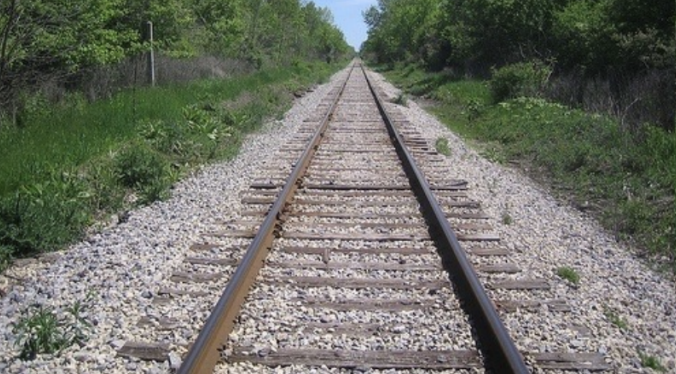
\includegraphics[scale=0.35]{figures/pic_1.png}
	\caption{一张风景图}
\end{wrapfigure}
上面我们解释了从3D转换到2D的过程,那么反过来,能否从单视角还原成3D呢?很显然,这并不是一个有唯一解的问题.无论是从维度的角度,还
是实际操作角度都是如此.成像的时候,一个pixel代表着一条射线,而其深度无法确定.

尽管如此,我们还是能得到一些有意思的结论.比如我们知道点会映射成点,而线映射成线.以及右图中,似乎铁轨和草皮交于图像上方的一点.


\section{Transformation in $\mathbb R^2$}

我们先来看看二维平面中的线.对于$ax+by+c = 0$,用齐次坐标表达为$l = [a, b, c]^\top$,则点在线上等价于$\bm x^\top l = 0$.这里$x = [x, y, 1]^\top$为齐次坐标.两条线$l, l^\prime$的交点坐标是$\bm x = \bm l \times \bm l^\prime$.

我们还能发现,这样的表示还能适用于平行线的交点.不难看出两条平行线的叉乘
\begin{equation}
	\begin{vmatrix}
		\bm i & \bm j &\bm k
		\\
		a & b & c
		\\
		a^\prime & b^\prime & c^\prime
	\end{vmatrix}
\end{equation}

的齐次坐标$ab^\prime - a^\prime b = 0$.$x_\infty = [b, -a, 0]^\top$.不难验算得到所有与这条直线平行的点都交于$x_\infty$.

我们还可以定义$1_\infty = [0, 0, 1]^\top$.这条线是所有无穷点的共线,即无穷远处的直线.这是在欧式空间无法表达的一条直线.其齐次坐标当然也可以是任何常数.

我们尝试将射影变换\footnote{附录\ref{transformation}当中简单介绍了几种变换的形式和性质.}作用于某个无穷远点,得到如下结果:
\begin{equation}
	\bm p^{\prime}=\bd H \bm p_{\infty}=\begin{bmatrix}
		\bd A & \bm t \\
		\bm v  & b
	\end{bmatrix}
	\begin{bmatrix}
		a \\
		b \\
		0
	\end{bmatrix}=
	\begin{bmatrix}
		p_{x}^{\prime} \\
		p_{y}^{\prime} \\
		p_{z}^{\prime}
	\end{bmatrix}
\end{equation}

也就是说,无穷远点可能会被映射到某个有限远的点.但是对于仿射变换,就不存在这种问题了:
\begin{equation}
	\bm p^{\prime}=\bd H \bm p_{\infty}=\begin{bmatrix}
		\bd A & \bm t \\
		\bm 0^\top & 1
	\end{bmatrix}
	\begin{bmatrix}
		a \\
		b \\
		0
	\end{bmatrix}=
	\begin{bmatrix}
		p_{x}^{\prime} \\
		p_{y}^{\prime} \\
		0
	\end{bmatrix}
\end{equation}

对于变换后的直线,根据射影变换的性质,如果将$\ell$变换为$\ell^\prime$,那么如果$\bm x \in \ell$,则$\bm x^\prime = \bd H \bm x \in \ell^\prime$.设对直线的变换是$\bd T$,那么有
\begin{equation}
	\bm x^{\prime \top} \bd T \ell=\bm x^{\top} \bd H^{\top} \bd H^{-\top} \ell=0
\end{equation}
得出$\bd T = \bd H^{-\top}$.同样我们可以发现射影变换可能会将无穷远处的直线映射到有限远,而仿射变换不会.

\section{Vanishing Points}

有了上面的铺垫,我们来看看vanishing point的概念.我们可自然地将上述概念推广到三维的情形,那么对三维空间中一系列平行线的无穷远点$\bm x_\infty$,经过相机变换$\bd M$,就会成为二维中的有限远的一个点$\bm p_\infty$,也就是vanishing point,如下图:
\begin{figure}[htbp]
	\centering
	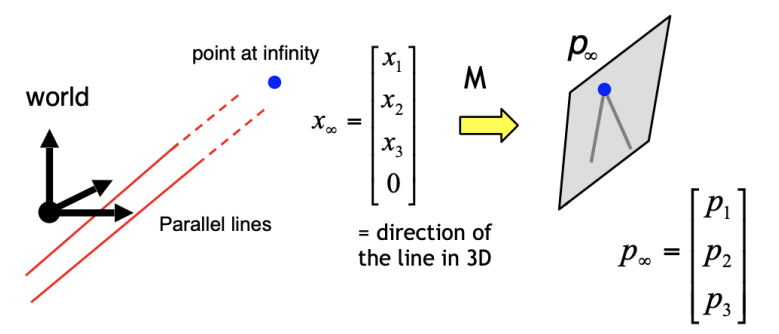
\includegraphics[scale=0.65]{figures/vanishingpoints.png}
	\caption{Vanishing points在world coordinate中的示意图}
	\label{}
\end{figure}

\begin{wrapfigure}{r}{4cm}
	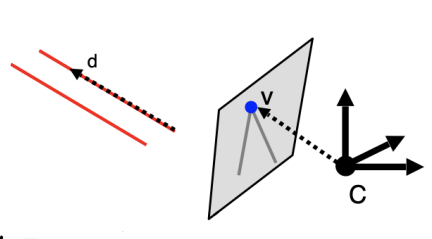
\includegraphics[scale=0.5]{figures/vpanddir.png}
	\caption{相机坐标下的方向}
\end{wrapfigure}
上图的坐标是world coordinate当中.如果是在camera coordinate当中,设$\bm d = (a, b, c)$是直线的方向向量,$\bm v$代表消失点,我们还可以导出如下关系\footnote{注意在右图里,$\bm v$并不是从相机坐标中心出发的三维矢量,而是图片坐标下的齐次坐标.}:
\begin{equation}
	\bm v = \bd K \bm d
\end{equation}


这一点不难证明:由于是在相机坐标之下,无需考虑extrinsic参数,直接有
\begin{equation}
	\bm v = \bd M \bm x_\infty = \bd K 
	\begin{bmatrix}
		\bd I & \bm 0
	\end{bmatrix}
	\begin{bmatrix}
		a\\b\\c\\0
	\end{bmatrix} = \bd K \bm d
\end{equation}

这样,如果已知vanishing point的坐标和相机参数,我们可以知道相机坐标下的这一组平行线的方向:
\begin{equation}
	\bm d = \frac{\bd K^{-1} \bm v}{\norm{\bd K^{-1} \bm v}}
\end{equation}






\begin{wrapfigure}{r}{4cm}
	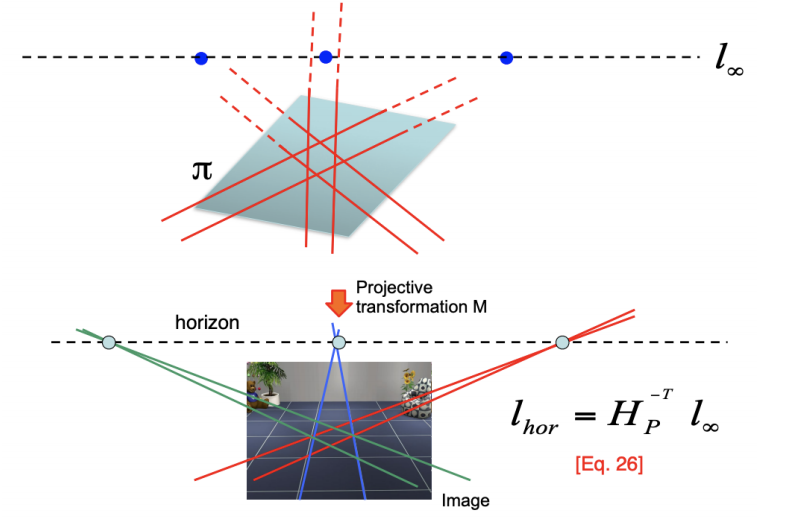
\includegraphics[scale=0.35]{figures/horizon.png}
	\caption{天际线}
\end{wrapfigure}

如果我们继续推广在二维空间中的结论,那么一系列平行平面将会相交于无穷远处的一条线$l_\infty$.将这条线也作同样的变换,就可以得到Vanishing Line,即Horizon,译为天际线,也就是3维空间$l_\infty$在二维的投影:
\begin{equation}
	l_{\text{hor}} = \bd H^{-\top} l_{\infty}
\end{equation}


通过这种方式,我们可以确定两条线是否平行.首先找出天际线,如果照片上的两条线交于天际线的同一点则平行,反之不平行.

我们还可以通过两个vanishing point确定其对应的平行线之间的夹角.

\begin{wrapfigure}{r}{4cm}
	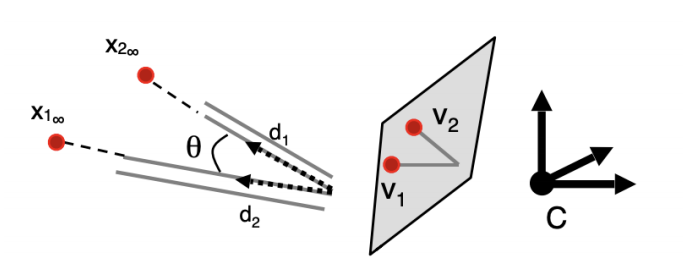
\includegraphics[scale=0.4]{figures/angle_between_line.png}
	\caption{Angle from two vanishing points.}
\end{wrapfigure}

如右图,根据$\bm d = \bd K^{-1} \bm v$,我们可以求出其夹角:
\begin{equation}
	\cos \theta = \frac{\bm d_1 \cdot \bm d_2}{\norm{\bm d_1} \norm{\bm d_2}}
\end{equation}



令$\bm \Omega =\left(K K^{T}\right)^{-1}$,得到
\begin{equation}
	\cos \theta=\frac{\bm{v}_{1}^{\top} \bm \Omega \bm{v}_{2}}{\sqrt{\bm{v}_{1}^{\top} \bm \Omega \bm{v}_{1}} \sqrt{\bm{v}_{2}^{\top} \bm \Omega \bm{v}_{2}}}  
\end{equation}

当$\theta = \frac{\pi}{2}$的时候有$\bm{v}_{1}^{\top} \bm \Omega \bm{v}_{2} = 0$.$\bm \Omega$有五个独立变量.如果我们已知空间中的三组互相垂直的平行线和它们在图片上的vanishing point,则我们可以获得三个方程
\begin{equation}
	\begin{cases}
		\bm{v}_{1}^{\top} \bm \Omega \bm{v}_{2} = 0
		\\
		\bm{v}_{1}^{\top} \bm \Omega \bm{v}_{3} = 0
		\\
		\bm{v}_{2}^{\top} \bm \Omega \bm{v}_{3} = 0
	\end{cases}
\end{equation}

如果我们假定相机具有零偏置和方形像素,那么不难得到
\begin{equation}
	\bd K = 
	\begin{bmatrix}
		\alpha & 0 & c_x
		\\ 
		0 & \alpha & c_y
		\\
		0 & 0 & 1
	\end{bmatrix}, \quad
	\bd K \bd K^{\top} = 
	\begin{bmatrix}
		\alpha^2 + c_x^2 & c_x c_y & c_x
		\\
		c_x c_y & \alpha^2 + c_y^2 & c_y
		\\
		c_x & c_y & 1
	\end{bmatrix}
\end{equation}
\begin{equation}
	\bd \Omega = \xk{\bd K \bd K^{\top}}^{-1} = \frac{1}{\alpha^4}
	\begin{bmatrix}
		\alpha^2 & 0 & -\alpha^2 c_x
		\\
		0 & \alpha^2 & -\alpha^2 c_y
		\\
		-\alpha^2 c_x & -\alpha^2 c_y & (\alpha^2 + c_x^2)(\alpha^2 + c_y^2) - c_x^2 c_y^2
	\end{bmatrix}
\end{equation}

$\bm \Omega$的形式变为:
\begin{equation}
	\bm \Omega = 
	\begin{bmatrix}
		\omega_1 & 0 & \omega_4
		\\
		0 & \omega_1 & \omega_5
		\\
		\omega_4 & \omega_5 & \omega_6
	\end{bmatrix}
\end{equation}

四个变量,三个线性方程,在常数倍意义下我们可以得到$\bd \Omega$,随后运用Cholesky分解得到$\bd K$.之后我们就可以对场景进行三维重建,例如计算图片中所有平面的方向,因此一张图片实际上蕴含了周围场景的丰富信息.

在这一节的最后,我们仍然要指出,单纯从一张图片是不可能完整重建原3D场景的,这是因为物体的深度和大小之间存在ambiguity.在下一节当中,我们会试图解决这个问题.
	\chapter{Epipolar Geometry}

\textbf{这一章节在2024年教学中已经被删去,为了让有兴趣的读者了解,故保留}

\begin{wrapfigure}{r}{4cm}
	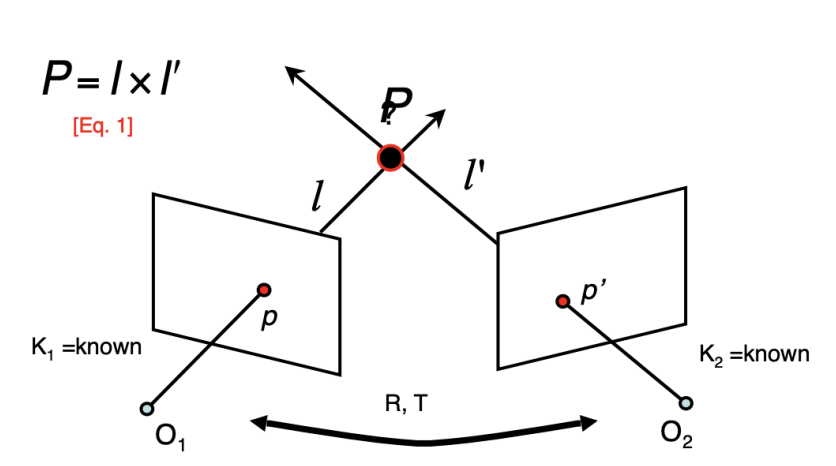
\includegraphics[scale=0.3]{figures/triangulation.png}
	\caption{Triangulation}
\end{wrapfigure}

既然单个视角无法确定深度,那么我们自然会想到如果有多台相机或许就可以确定距离,如同人眼一样.

原则上,两台相机就可以确定点的位置.我们看右图:$O_1, O_2$代表两台相机的镜心,两个平行四边形代表各自的像平面,如果一个点$P$在两个像平面的投影点$p, p^\prime$已知,我们就可以确定$P$点在镜心到对应点的连线交点的位置.

在前面的章节当中我们已经介绍了校准相机的方法,而两台相机的位置参数$\bd R, \bm t$一般都是已知的,此时的关键问题就是:\textbf{确定一个点在另一个相机图片的位置}.



\begin{figure}[htbp]
	\centering
	\subfigure[对极几何中的基本概念]{
		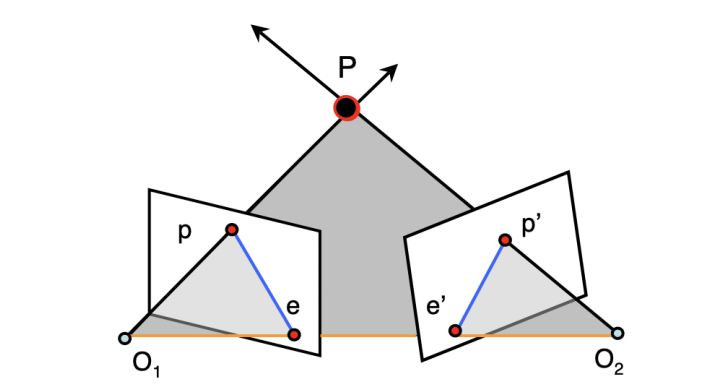
\includegraphics[scale=0.45]{figures/epipolargeometry.png}
	}
	\subfigure[像平面平行的情形]{
		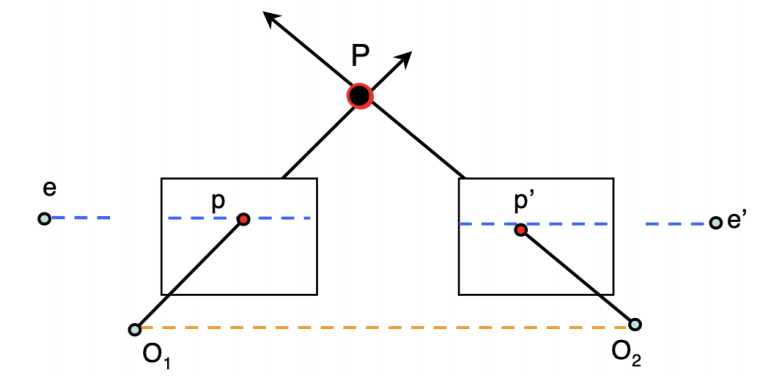
\includegraphics[scale=0.45]{figures/parallel-image-plane.png}
	}
\end{figure}

与这一任务相关的几何内容被称为对极几何(epipolar geometry).我们先给出对极几何当中的一些概念.

左图中由$O_1, O_2, P$三点构成的平面(图中灰色填充)被称为epipolar plane.连线$O_1O_2$被称为baseline.baseline与两个像平面的交点被称为epipole.各个像平面内,epipole与$P$的投影点被称为epipolar line.

当$P$点移动时,相当于极平面上下翻动,此时对应的极线也会变化,但是所有的极线都通过极点.

一种特殊情况是两个像平面相互平行,此时极点位于无穷远处,图中所有极线都平行于基线.
那么,给定图片中的一个点,要如何去确定在另一张图片中这个点的对应呢?我们看下图,根据给定点和基线我们可以确定极平面,极平面与右像平面的交点即为极线,对应点$p^\prime$必定在此极线上,也就将对应点的搜索从2维降低到了1维.
\begin{figure}[htbp]
	\centering
	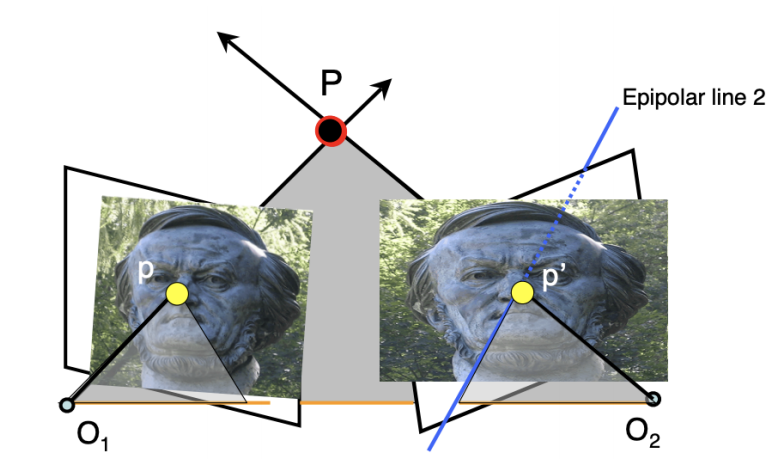
\includegraphics[scale=0.45]{figures/epi-geo-2pic.png}
	\caption{两张图片的对应}
\end{figure}

\section{Epipolar Constrain}
首先我们先确定两台相机的位置.如下图,方便起见,假设世界坐标与第一台相机的坐标重合,第二台相机的坐标系由旋转$\bd R$和偏置$\bm t$确定.对于一点$\bm P$,如果它在两台相机的坐标系下的坐标分别是$\bm p_E, \bm q_E$,则有关系
\begin{equation}
	\bm q_E = \bd R^{\top}\xk{\bm p_E - \bm t}
\end{equation}

因此,两台相机的变换矩阵分别是
\begin{equation}
	\bd M = \bd K
	\begin{bmatrix}
		\bd I & \bm 0
	\end{bmatrix} ,
	\quad
	\bd M^\prime = \bd K^\prime
	\begin{bmatrix}
		\bd R^{\top} & \bm -\bd R^{\top} \bm t
	\end{bmatrix}
\end{equation}


\begin{figure}[htbp]
	\centering
	\subfigure[两台相机的位置]{
		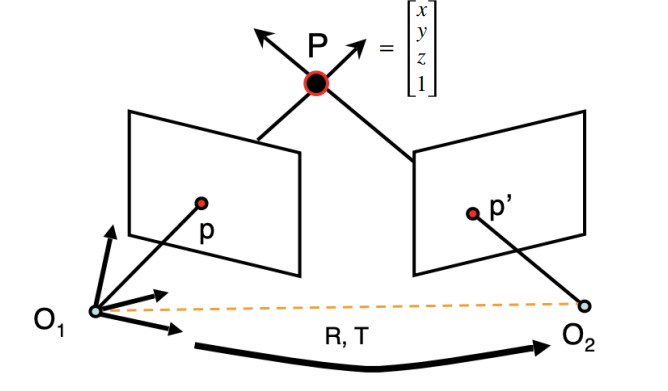
\includegraphics[scale=0.45]{figures/epi-constrain.png}
	}
	\subfigure[坐标变换]{
		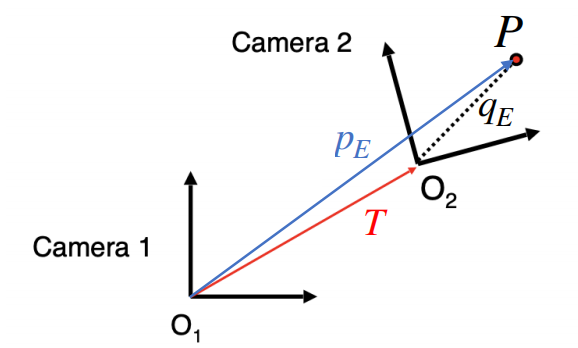
\includegraphics[scale=0.45]{figures/camata-pose.png}
	}
	\subfigure[对极约束]{
		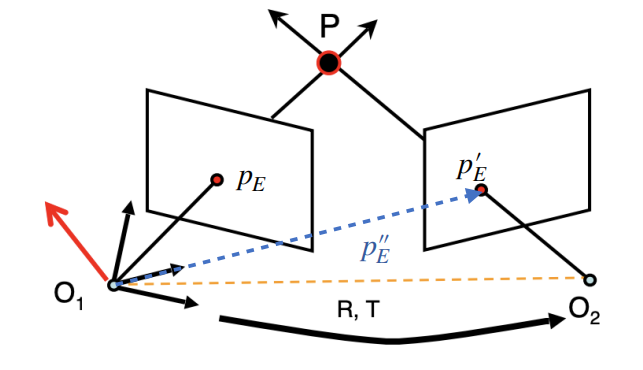
\includegraphics[scale=0.45]{figures/epi-constrain-2.png}
		\label{fig:epi-constrain-2}
	}
	\caption{}
\end{figure}

如图 \ref{fig:epi-constrain-2} ,我们规定以下符号:$\bm p_E, \bm p_E^\prime, \bm p_E^{\prime\prime} \in \mathbb R^3$分别代表左投影点在左相机坐标系(即世界坐标系)的坐标,右投影点在右相机坐标系下的坐标,右投影点在左相机坐标系下的坐标.我们可以求出极平面的法向量(图中红色箭头):
\begin{equation}
	\bm n = \bm t \times \bm p_E^{\prime\prime} = \bm t \times \xk{\bd R \bm p_E^{\prime} + \bm t} = \bm t \times \bd R \bm p_E^{\prime}
\end{equation}

对于两个向量$\bm a = [a_x, a_y, a_z]^\top, \bm b = [b_x, b_y, b_z]^\top$的叉乘,可以表示成矩阵形式:
\begin{equation}
	\bm a \times \bm b  = \zk{\bm a_{\times}}\bm b = 
	\begin{bmatrix}
		0 & - a_z & a_y
		\\
		a_z & 0 & -a_x
		\\
		-a_y & a_x & 0
	\end{bmatrix}
	\begin{bmatrix}
		b_x
		\\
		b_y
		\\
		b_z
	\end{bmatrix}
\end{equation}
不难看出这是一个反对称矩阵,秩为$2$.

显然有$\bm p_E \perp \bm n$,写成矩阵形式就是

\begin{equation}
	\bm p_E^\top \zk{\bm t_{\times}}\bm R \bm p^{\prime}_E = 0
	\label{eq:essential-matrix}
\end{equation}

我们定义
\begin{equation}
	\bd E = \zk{\bm t_{\times}}\bm R
\end{equation}
为本质矩阵(essential matrix).它是一个形状为$3 \times 3$,秩为$2$的矩阵,有五个自由度.\footnote{在下文的基本矩阵的讨论中,我们也会涉及到自由度的问题,这一度令笔者陷入困惑.这些内容将在附录 \ref{DOFandRank} 当中作进一步探讨.}

代入式 \ref{eq:essential-matrix}得到:
\begin{equation}
	\bm p_E^\top \bd E \bm p^{\prime}_E = 0
\end{equation}

虽然有了本质矩阵是在两个相机坐标系下的三维坐标的变换,我们自然希望能用二维的图片坐标进行直接对应.考虑到
\begin{equation}
	\bm p_E = \bd K^{-1} \bm p, \quad \bm p_E^\prime = \bd K^{\prime-1} \bm p^\prime
\end{equation}

代入式 \ref{eq:essential-matrix}即得
\begin{equation}
	\bm p^\top \bd K^{-\top} \zk{\bm t_{\times}}\bd R \bd K^{\prime-1} \bm p^{\prime} = 0
\end{equation}

我们定义
\begin{equation}
	\bd F = \bd K^{-\top} \bd E \bd K^{\prime-1} = \bd K^{-\top} \zk{\bm t_{\times}}\bd R \bd K^{\prime-1}
	\label{eq:fundamental-matrix}
\end{equation}
为基本矩阵(fundamental matrix),它是一个秩为$2$,自由度为$7$的$3 \times 3$矩阵.式 \ref{eq:fundamental-matrix}变为
\begin{equation}
	\bm p^\top \bd F \bm p^{\prime} = 0
	\label{eq:fundamental-mat}
\end{equation}


\begin{wrapfigure}{r}{6cm}
	\centering
	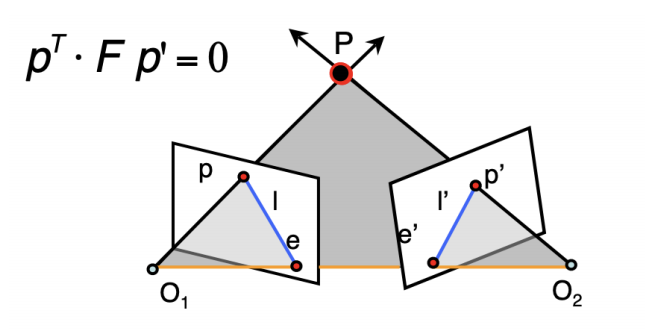
\includegraphics[scale=0.55]{figures/property-of-f-mat.png}
	\caption{基本矩阵的性质}
	\label{fig:property of fundamental matrix}
\end{wrapfigure}

除此之外,基本矩阵还有如下性质:如图 \ref{fig:property of fundamental matrix},首先,$l = \bd F \bm p^\prime$和$l^\prime = \bd F^{\top} \bm p$分别是$\bm p, \bm p^\prime$对应的极线.其次,$\bd F \bm e^\prime = 0, \bd F^\top \bm e = 0.$

先证明前者.式 \ref{eq:fundamental-mat}说明$\bm p \in l$.设$\bm e$对应的世界坐标为$\bm e_E$,则由于$\bm e_E \perp \bm n$,因此式 \ref{eq:essential-matrix}及以后的各式将$\bm p_E$替换成$\bm e_E$都成立,那么同式 \ref{eq:fundamental-mat}的形式,我们亦可以得到

\begin{equation}
	\bm e^\top \bd F \bm p^{\prime} = 0.
	\label{eq:all points in epipolar plane}
\end{equation}

由此得出$\bm e \in l$.\footnote{细心的读者不难发现,极平面内所有的点都可以这样做,而这个结论也是非常自然的,因为极线正是极平面射影在左像平面的结果.}

对于后者,我们知道$\forall \bm p$,都有式 \ref{eq:all points in epipolar plane}成立,因此只能有
\begin{equation}
	\bd F \bm e^\prime = 0, \quad \bd F^\top \bm e = 0.
\end{equation}

我们对本质矩阵和基本矩阵做一个总结.

$\bd E$是两个标准相机相对关系的内参,换言之,给定两个已标定相机的相对位置关系,$\bd E$即被确定.

$\bd F$是任意两个相机相对关系的内参,换言之,给定了两个相机的相对位置关系和相机内参,$\bd F$即被确定.

如果我们能够求出$\bd F$,那么就可以在不进行三维重建的情况下,确定两张照片的对应关系.还记得我们在上节末尾和这节的开头提出的问题吗?在上一节的末尾,我们说通过两台相机即可确定深度信息,在这一节的开头我们引入了对极几何的概念,我们的目的是确定两张照片中的对应点,再通过两台相机的方向即可求出点的深度,而方向已经在上一节中解决.现在我们离解决这个问题只剩最后一步,即如何求出$\bd F$?

我们设$\bd F = (F_{ij})$,根据式 \ref{eq:fundamental-mat},如果有8对对应点\footnote{这里读者可能会产生一个问题,既然$\bd F$的自由度为$7$,为什么要8对对应点呢?其中原因之一是,相机的内部性质多为非线性,所以使用最小点数求解可能会比较麻烦,因此经常只考虑尺度的等价性,忽略奇异性条件,此时自由度为8.}的坐标$(u_i, v_i, 1)^{\top} \leftrightarrow (u_i^\prime, v_i^\prime, 1)^{\top}$, 那么我们可以得到方程组
\begin{equation}
	\begin{pmatrix}
		u_{1} u_{1}^{\prime} & u_{1} v_{1}^{\prime} & u_{1} & v_{1} u_{1}^{\prime} & v_{1} v_{1}^{\prime} & v_{1} & u_{1}^{\prime} & v_{1}^{\prime} & 1 \\
		u_{2} u_{2}^{\prime} & u_{2} v_{2}^{\prime} & u_{2} & v_{2} u_{2}^{\prime} & v_{2} v_{2}^{\prime} & v_{2} & u_{2}^{\prime} & v_{2}^{\prime} & 1 \\
		u_{3} u_{3}^{\prime} & u_{3} v_{3}^{\prime} & u_{3} & v_{3} u_{3}^{\prime} & v_{3} v_{3}^{\prime} & v_{3} & u_{3}^{\prime} & v_{3}^{\prime} & 1 \\
		u_{4} u_{4}^{\prime} & u_{4} v_{4}^{\prime} & u_{4} & v_{4} u_{4}^{\prime} & v_{4} v_{4}^{\prime} & v_{4} & u_{4}^{\prime} & v_{4}^{\prime} & 1 \\
		u_{5} u_{5}^{\prime} & u_{5} v_{5}^{\prime} & u_{5} & v_{5} u_{5}^{\prime} & v_{5} v_{5}^{\prime} & v_{5} & u_{5}^{\prime} & v_{5}^{\prime} & 1 \\
		u_{6} u_{6}^{\prime} & u_{6} v_{6}^{\prime} & u_{6} & v_{6} u_{6}^{\prime} & v_{6} v_{6}^{\prime} & v_{6} & u_{6}^{\prime} & v_{6}^{\prime} & 1 \\
		u_{7} u_{7}^{\prime} & u_{7} v_{7}^{\prime} & u_{7} & v_{7} u_{7}^{\prime} & v_{7} v_{7}^{\prime} & v_{7} & u_{7}^{\prime} & v_{7}^{\prime} & 1 \\
		u_{8} u_{8}^{\prime} & u_{8} v_{8}^{\prime} & u_{8} & v_{8} u_{8}^{\prime} & v_{8} v_{8}^{\prime} & v_{8} & u_{8}^{\prime} & v_{8}^{\prime} & 1
	\end{pmatrix}
	\begin{pmatrix}
		F_{11} \\
		F_{12} \\
		F_{13} \\
		F_{21} \\
		F_{22} \\
		F_{23} \\
		F_{31} \\
		F_{32} \\
		F_{33}
	\end{pmatrix}
	= \bm 0
	\label{eq:8 points to solve F}
\end{equation}

我们记上式为
\begin{equation}
	\bd W \bm f = \bm 0
\end{equation}

如果$\text{rank}(\bd W) = 8$,则$\bm{f}$有唯一非零解.当对应点对数目多于$8$个,则限制$\norm{\bm f} = 1$,使用SVD求解.但是$\bd F$的秩为$2$,那么问题转化为
\begin{equation}
	\begin{aligned}
		\text{minimize } &\norm{\bd F - \hat{\bd F}}
		\\
		\st &  \det{\bd F} = 0.
	\end{aligned}
\end{equation}

而SVD告诉我们,设$\text{rank}(\bd F) = r,$若将$\bd F$按奇异值降序分解为
\begin{equation}
	\bd F = \sum_{i=1}^{r} \sigma_i \bm u_i \bm v_i^\top
\end{equation}

则在所有秩不大于$k$的矩阵当中,
\begin{equation}
	\bd F = \sum_{i=1}^{k} \sigma_i \bm u_i \bm v_i^\top
\end{equation}
就是使得$\norm{\bd F - \hat{\bd F}}$最小的矩阵.因此我们需要对式 \ref{eq:8 points to solve F}求解出的$\bd F$再次进行SVD,并取前两个奇异值和左右奇异向量构成解$\bd{F}$.
	\chapter{3D Data}

\section{Sensors}

\textbf{\\第一种sensor:Depth Sensors}

得到的是一个深度图, 但是深度图RGBD是2.5D的, 如果不知道相机内参,不能完全表示3D的信息

\textbf{\\第二种sensor:Stereo Sensors}

Pros:

\begin{enumerate}
    \item Robust to the illumination of direct sunlight
    \item Low implementation cost
\end{enumerate}

Cons:

\begin{enumerate}
    \item Finding correspondences along $\text{Image}_L$ and $\text{Image}_R$ is hard and erroneous
\end{enumerate}

可以升级为Active Stereo, 之前的双目相机是passive, 现在看看打光的主动识别, 在两个相机之外加入一个红外线发射器

但是红外线主动 sensor 仅限于室内使用, 室外使用会受到阳光的干扰, 并且不能处理透明或者非漫反射的物体

\textbf{\\第三种sensor:time-of-light}

即用光的传播时间计算距离, 具体有如下两种

dTOF(direct Time of Flight)
\begin{enumerate}
    \item 发射脉冲波, 通过光的传播时间计算距离, 被认为是比iTOF更好的方法
    \item 理论上精度高, 但是现在分辨率还很低
    \item 对器件要求高, 需要使用SPAD (单光子雪崩二极管), 无法做得很密集, 造价高
\end{enumerate}

iTOF(indirect Time of Flight)
\begin{enumerate}
    \item 发射正弦波,通过光的相位差计算距离
    \item 精度低 (误差与距离成正比), 但是分辨率高
    \item 造价低
\end{enumerate}

\textbf{Summary of Different Depth Sensors}

\begin{figure}
    \centering
    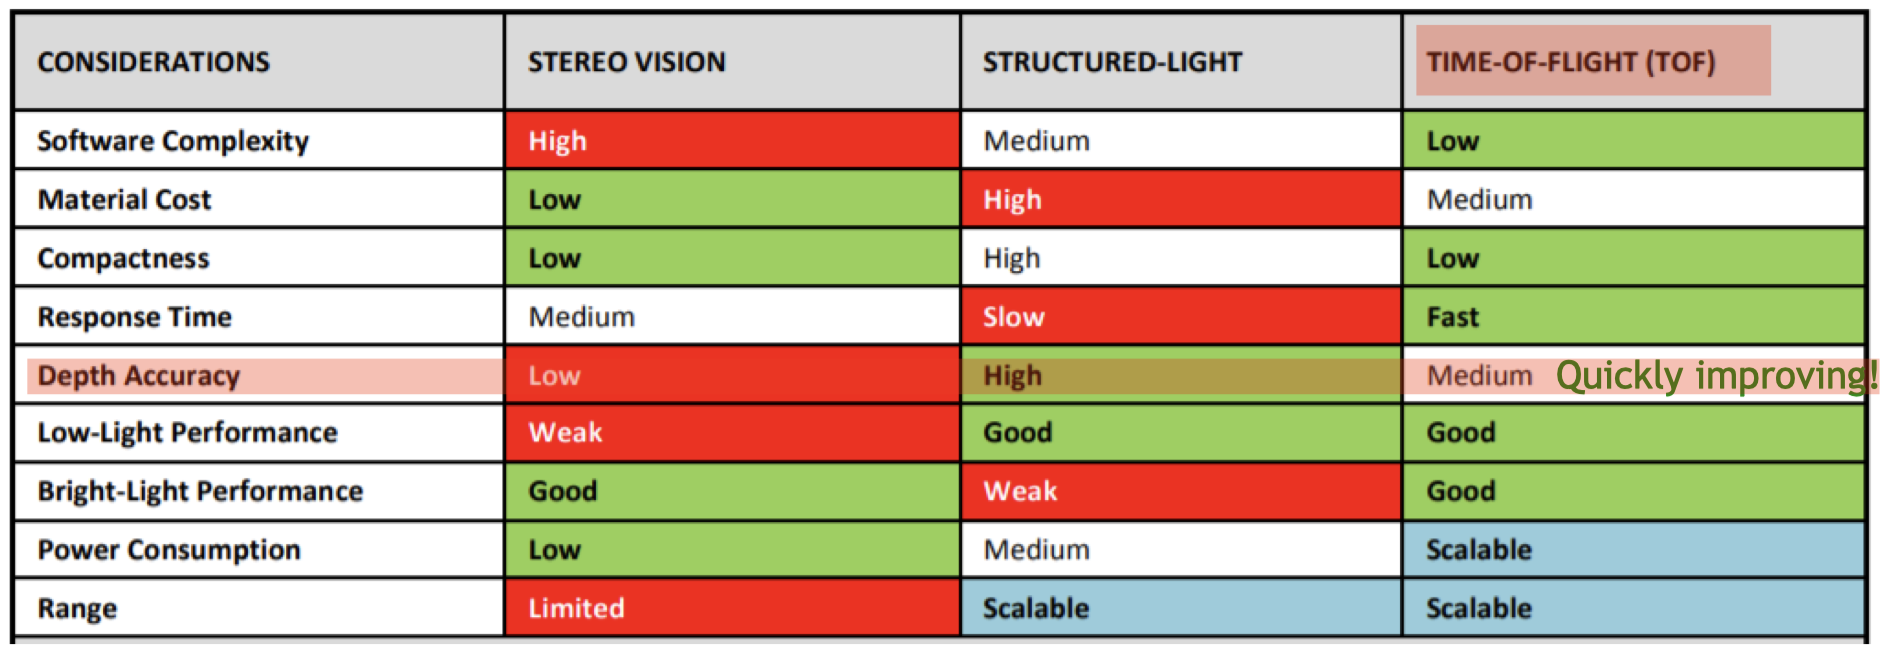
\includegraphics[width=0.7\textwidth]{figures/sensors.png}
    \caption{Summary of Different Depth Sensors}
\end{figure}

\section{Multiple 3D representation}

\begin{enumerate}
    \item Multiple images.从各个视角获得的多张图片.它包含3D信息,indirect,not a true 3D representation.
    \item Depth image.只知道深度,不知道相机内参,无法确定两个点的距离.因此被称为2.5D.
    \item Voxels.物体占据了位置则设为1.能被index.但是非常昂贵.$O(n^3)$.没有表面的表示.一旦分辨率低,则无法还原丢失的信息.
    \item Irregular 3D representation. Mesh,point Cloud, Implicit representation.
\end{enumerate}

\section{Mesh}

在表面取点,用过三点的平面近似表面.实际上也不限于三角形.下面我们讨论triangle mesh.

\begin{equation}
    \begin{aligned}
        V &= \{v_1, \cdots, v_n\} \in \mathbb R^3
        \\
        E &= \{e_1, \cdots, e_n\} \in V\times V
        \\
        F &= \{f_1, \cdots, f_n\} \in V\times V \times V
    \end{aligned}
\end{equation}


好的mesh:watertight(不漏), manifold(外法向量连续).

\section{Point Cloud}

Point cloud是一个$3n$级别的存储方式,当然也可以添加其他分量.它是不规则(irregular)且无序的数据.换言之,其数据的序并不是必要的,
不能提供额外信息,如同set一样.好的算法应该尽可能不去运用序.它是非常轻量级,紧致的,线性级别的存储空间.容易存储,容易理解和生成,容易在其上构建算法.

当然它也不是完美的,比如并不容易通过它判断表面的位置.点云实际上是在表面上采样,那么怎样从一个mesh surface上取样呢?

\textbf{Sampling Strategy:Uniform Sampling.}
计算每个表面的面积,以面积为权独立同分布地选取三角形.在三角形里如何均匀选取呢?仿射变换形成直角三角形,再拼接成矩形.
\footnote{直接拼接成平行四边形如何?对三角形均匀采样可以在正方形 (平行四边形)中采样然后对角线截半.}

但是这样取样之后,在取样量不算非常大的时候,经常会出现不太均匀的情形.此时我们可以采用Farthest Point Sampling(FPS).
目标是选取$N$个点使其两两距离求和最大.但这是一个$\mathcal{NP}$-hard的问题.我们采取一个近似的贪心算法.
我们先均匀选取10000个点.在这10000个点最远的1024个点成为组合优化问题.但仍然比较困难.我们先确定一个点,
最后依次选取最远的点.我们也只是希望点云看起来比较均匀,因此没必要一定取得数学上的最优解.

除此之外,点云的距离度量也成为一个问题,这也是无序带来的问题之一.
我们希望找到一个permutation invariant的度量:Chamfer distance.
\footnote{在某些文献当中,式 \ref{eq:chamfer distance}有时也会带平方.
但是如果带平方,则三角不等式不成立.}

\begin{equation}
    d_{CD} = \sum_{x \in S_1} \min_{y \in S_2} \norm{x - y}_{2} + \sum_{y \in S_2} \min_{x \in S_1} \norm{x - y}_{2}
    \label{eq:chamfer distance}
\end{equation}

对于每个单项,称为uni chamfer distance.在一个点云是另一个子集的时候有用.并且这里似乎应该除以二才能和EMD进行比较.

另一个度量是Earth Mover's distance\footnote{在WGAN中使用.}.与CD不同的是,它要求两个点云数量相同,
且每个点必须找到互不重复的对应.\footnote{Earthmover,中文直译为推土机.
EMD距离用于衡量(在某一特征空间下)两个多维分布之间的dissimilarity,它
的计算基于著名的运输问题.但是精确求解EMD亦非易事,调用的package也多为近似算法.}

\begin{equation}
    d_{E M D}\left(S_{1}, S_{2}\right)=\min _{\phi: S_{1} \rightarrow S_{2}} \sum_{x \in S_{1}} \norm{x-\phi(x)}_{2}
\end{equation}

CD对于取样情况不太敏感,而EMD则比较敏感.比如同样对于Stanford bunny,
如果一个点云多集中在头部,另一个比较均匀,则CD变化不大而EMD变换显著.
由于点云是surface+sampling,因此如果对于取样有要求,应该使用EMD.

\section{CD vs EMD}

区别在于 CD 对于采样不敏感,而 EMD 对于采样敏感.

同时EMD需要两个点云点的数量相同.

也就是如果mesh一样但是sample不一样,那么EMD会很大

\section{Implicit Representation}

对于一个点,使用一个关于这个点的函数的值来表示这个点是否在物体表面

具体的表示方法是隐式表达,即SDF(signed distance function)

简单地说,这个函数表示空间中点到物体表面的距离,内部为负,外部为正.

其数学定义为:设$\Omega$为度量空间$X$的子集,$d$为$X$的度量,则SDF定义为

\begin{equation}
    f(x)=\begin{cases}
        -d(x, \partial \Omega) & \text { if } x \in \Omega 
        \\
        d(x, \partial \Omega) & \text { if } x \in \Omega^{c}
    \end{cases}
\end{equation}

其中$d(x, \partial \Omega) \xlongequal{\text{def}} \inf_{y \in \partial \Omega} d(x, y)$.

SDF的用处:

\begin{enumerate}
    \item \textbf{collision check:}如果一个东西跟另外一个东西的碰撞.
    那么其中物体A它上面的所有点到底有没有碰到物体B呢?
    我们就可以通过query所有点在B的物体的SDF里头它的值是多少.如果都是大于0,说明A和B没有碰撞
    \item 使用神经网络把物体的几何通过SDF的方式存储下来
\end{enumerate}

\textbf{\\Mesh to SDF}

在处理Mesh到Signed Distance Field (SDF)的转换时,首先需要一些坐标点,
基于这些点的距离值,可以尝试开发算法来计算对应的SDF值

\paragraph{Calculate Unsigned Distance}
在几何处理中,一种基础的方法是计算点到表面的距离 (Unsigned Distance),不区分点是在物体内部还是外部.
这可以通过将所有三角面视为平面,对于每个点,计算其到每个三角面的垂线距离.如果垂足不在三角面上,
则该距离不是最短距离;如果垂足位于三角面上,则从这些距离中找出最短的,即为该点到表面的最短距离.

\paragraph{Unsigned Distance to Signed Distance}
要将Unsigned Distance转换为Signed Distance,使用等高线将空间中的点进行分层表示.
这些等高线描绘了在某些区域距离先减小然后增加,其中距离最近的点附近的区域距离为零,
利用距离为零的区域判断点是在物体的内部还是外部.

\textbf{\\SDF to Mesh}

使用 marching cube

\begin{figure}[H]
    \centering
    \begin{subfigure}
        \centering
        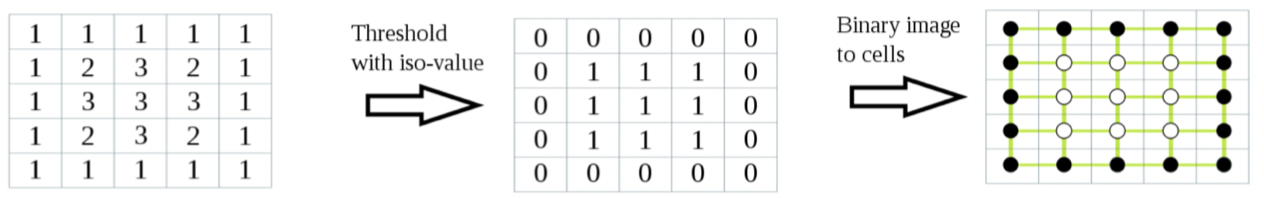
\includegraphics[width=0.7\textwidth]{figures/marching_cube1.png}
    \end{subfigure}
    \vspace{1em} % 调整两个子图之间的垂直间距
    \begin{subfigure}
        \centering
        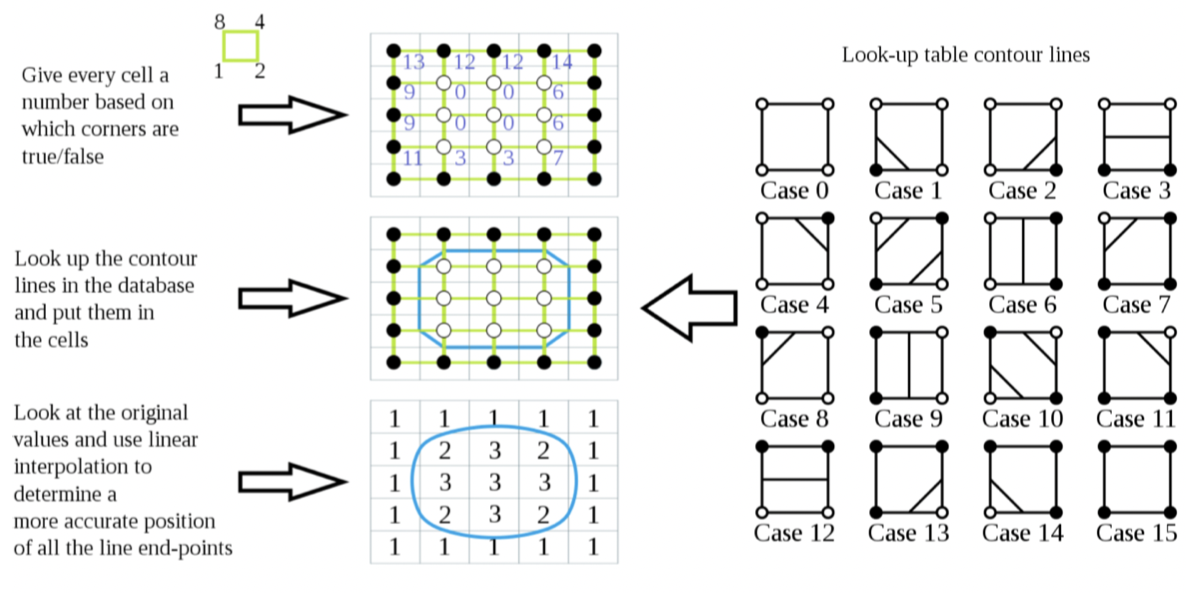
\includegraphics[width=0.7\textwidth]{figures/marching_cube2.png}
    \end{subfigure}
    \caption{Marching cube pipelines}
    \label{fig:marching_cube}
\end{figure}

\begin{enumerate}
    \item 离散化
    \item 二值化
    \item 使用look-up table找轮廓
    \item 使用线性插值优化轮廓
\end{enumerate}

在第三步,很多case都会有这种ambiguity, 如图\ref{fig:mesh reconstruction},所以还需要根据周围的mesh二次优化,决定ambuguity的位置,对于三维mesh重建,这个问题更加严重.

\begin{figure}[H]
    \centering
    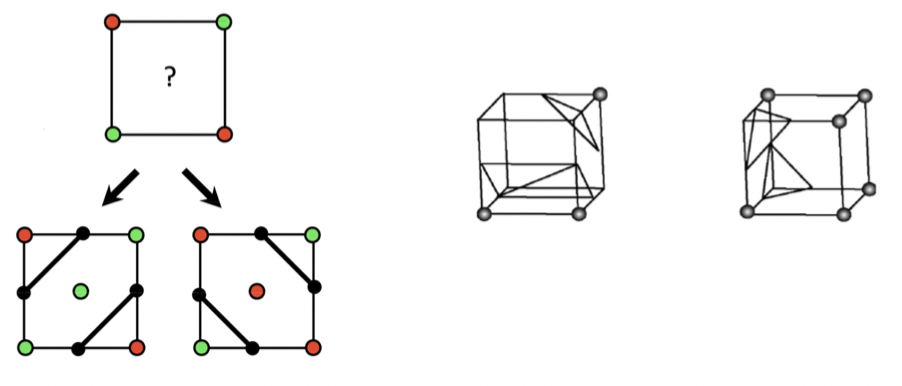
\includegraphics[width=0.7\textwidth]{figures/holes.png}
    \caption{Problem in mesh reconstruction}
    \label{fig:mesh reconstruction}
\end{figure}

\section{Deep SDF}

两个trick:

1. 如何分布训练数据点: 如果这个神经网络SDF最终需要使用marching cube,那么应该在SDF为0附近多多采样

2. 训练loss的设置,可以加入一个约束优化:让SDF的梯度为1.这样可以让SDF更加smooth

SDF还满足Eikonel equation,即

\begin{equation}
    \norm{\nabla F} = 1.
\end{equation}

这点不难理解,因为沿与距离最短的点的连线方向的方向导数之模为$1$,而函数本身即表达最短距离, 也就是场变化最快的方向,
不可能沿着梯度前进一个单位的长度,距离变化却超过一单位,因此这也是最大值.

将不同的SDF关联起来,并且保证连续性\cite{Park2019CVPR}

\begin{enumerate}
    \item  use the network to overfit a single shape
    \item use a latent code to represent a shape, so that the
    network can be used for multiple shapes
\end{enumerate}

\section{NeRF, 3DGS, Convolution on Mesh/Graph}

了解即可
	\section{3D Deep Learning}

对于点云来说,直接拉成vector显然是不行的.因为点云本身无序.有一些直接的处理方法:转换成voxel grid(从点云到表面,再重建voxel),或者2D 投影(这属于是越活越回去了).我们想要的network需要对$N!$种不同的点云顺序具有不变性.

一种想法:排序赋予序关系如何?

我们用Permutation Invariant的函数:Symmetric Function.也就是
\begin{equation}
    f(x_1, x_2, \cdots, x_n) \equiv f(x_{\pi_1}, x_{\pi_2}, \cdots, x_{\pi_n}), \forall x \in \mathbb R^N
\end{equation}

实际上,这样的函数随处可见.比如均值,极值等.文献\cite{PointNet} 、PointNet.\footnote{王老师:"虽然我不在这个组里,但PointNet这篇论文的诞生我也是亲眼目睹过的,ICCV的投稿截止在11月,9月底大家还不知道投什么,于是有人说要不试试PointNet吧.写到最后只有两个周调参了,还是打不过voxel,于是加了T-transform.我们这里不讲,因为现在几乎没有用这个的了".(笑)}

\begin{figure}[htbp]
    \centering
    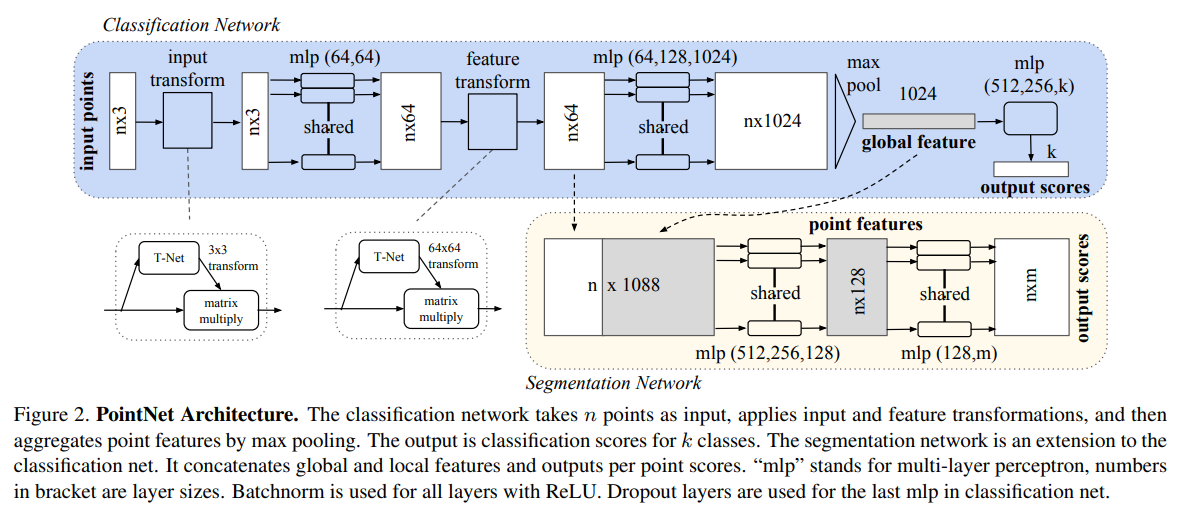
\includegraphics[scale=0.6]{figures/PointNet.png}
    \caption{PointNet的结构图}
\end{figure}

做segmentation:将每个点自身的特征(local)和global feature结合,过MLP就能进行分类.

诸多挑战:Resolution,Occlusion,Noise,Registration.

PointNet对于Resolution和Noise比较robust.在ModelNet40上,去掉50\%的数据,Furthest的准确率只下降了2\%.
能够如此稳定的关键在于max函数,在连续取样时,一些点的丢失可以用周围的点来弥补.而且如果pointnet只有1024个feature,
那么它最多也只会选取1024个点,可能去掉的点根本就没有用到.

\textbf{\\PointNet的不足}

一步直接maxpooling,没有local context.
但是PointNet仍是目前不追求过高性能时对point cloud处理的首选方法.

因为这个不足,有了PointNet++.
即设定一定的范围,将某个点及其周围的点过MLP,再maxpooling.等同于在image里进行conv.当然,求neighbour可能比较花时间.
另外,所有的neighbour都通过了同样的MLP,毕竟在点云里也无法和图像一样,使用卷积核直接提取局部特征.

\begin{figure}[htbp]
    \centering
    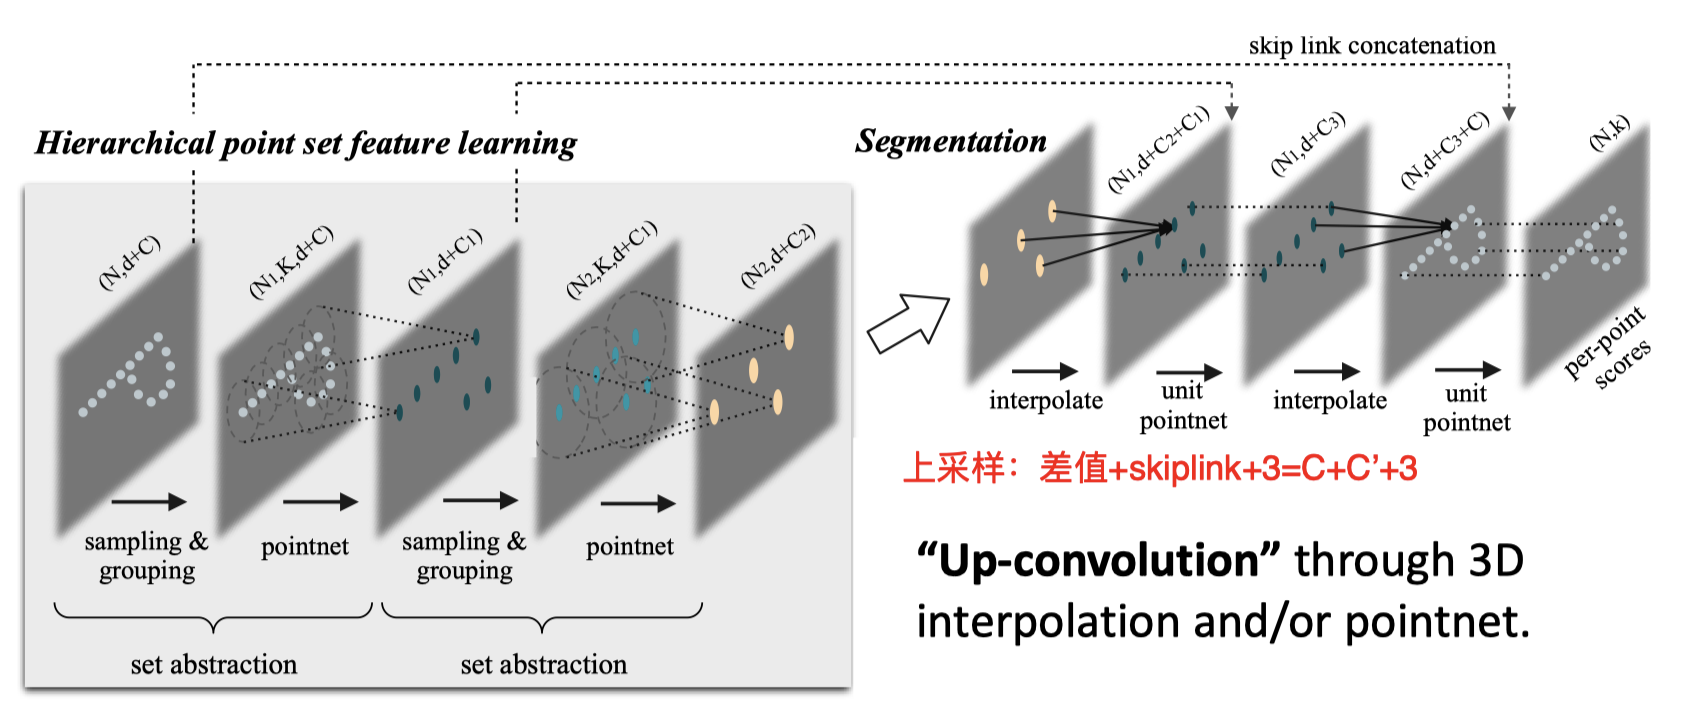
\includegraphics[scale=0.2]{figures/pointnet++.png}
    \caption{PointNet++ Pipeline}
\end{figure}

\textbf{\\PointNet++怎么进行下采样?} 2d中是pooling,而pointnet则进行grouping

\textbf{\\PointNet++怎么进行上采样?}
使用 Skip-Link,将下采样产生的点输入回来.

上采样时候添加的点没有feature, 所以进行interpolate,
新的点选择与它最近的三个点,按照距离反比为权插值获得特征, 这里skip-link是必要的, 否则无法获得点的具体位置.

\subsection{Sparse Conv}

3D:voxel Net$\rightarrow$sparse conv,屏蔽没有值的voxel,Hash有值的坐标,从NVIDIA,cuda的层次写起.

\begin{figure}[H]
    \centering
    \includegraphics[scale=0.2]{figures/sparsenet.png}
    \caption{Sparse Conv}
    \label{fig:sparsenet}
\end{figure}

结合图示\ref{fig:sparsenet}来理解稀疏卷积的过程:

\begin{enumerate}
\item 输入特征图:图中的红色方块表示非零值的位置,比如在输入特征图中,位置 (0,3)、(1,1)等具有非零值.
\item 卷积核:一个 3$\times$3 的卷积核,包含权重参数 $w_{-1,-1}$ 等.
\item 输出特征图:稀疏卷积的输出特征图.只有当卷积核的中心对准输入特征图的非零值时,才会计算输出值.
\item 稀疏卷积过程:当卷积核的中心对准输入特征图的 (0,3) 位置时,计算对应的输出值.
例如,卷积核中心对准 (0,3) 时,只有卷积核的中心权重 ($w_{0,0}$) 参与计算,输出值为:\[ \text{output}(0,3) = \text{input}(0,3) \times w_{0,0} \]
当卷积核中心对准 (1,4) 位置时,计算对应的输出值,输出值为:\[ \text{output}(1,4) = \text{input}(1,4) \times w_{1,1} \]
\item 通过这种方式,稀疏卷积仅计算非零值对应的输出,从而减少了大量的计算和内存开销.
\end{enumerate}

Sparse conv:kernel 是空间各向异性(spatial anisotropic)的.因此它的acc能够达到惊人的70\%以上,
而point cloud无论如何添加特性,最多也在64\%左右.而且因为可被标签,使用更加方便.但是它的分辨率受限.

\textbf{\\Sparse Conv Pros and Cons?}

Sparse Conv优点:
\begin{enumerate}
    \item 比dense conv更高效,稀疏卷积只对非零值进行计算,跳过零值,从而显著减少了计算量和内存使用,提高了计算效率.
    \item 支持索引的网格, 稀疏卷积仍然在规则的网格上操作,这意味着可以利用现有的索引机制来高效地访问数据.
    \item 与2D Conv具有类似的表达能力
    \item 与2D Conv具有类似的平移等变性
\end{enumerate}

Sparse Conv缺点:
\begin{enumerate}
    \item 离散化误差, 由于稀疏卷积只对非零值进行计算,可能会导致离散化误差.这种误差源于对数据的稀疏表示,可能会影响卷积操作的精确性.
\end{enumerate}

\textbf{\\Sparse Conv vs. Point Cloud Networks?}

Sparse Conv:
\begin{enumerate}
    \item 优点:核是空间各向异性的
    \item 优点:更高效的索引和近邻查询
    \item 优点:适用于大规模场景
    \item 缺点:分辨率有限
\end{enumerate}

Point Cloud Nets:
\begin{enumerate}
    \item 优点:分辨率高
    \item 优点:鲁棒性强
    \item 缺点:表现稍差一些
    \item 缺点:执行 Farthest Point Sampling 和 Ball Query 等操作较慢
\end{enumerate}

\subsection{PointNet++ V.S. Conv}

PointNet++相当于卷积网络的先做 $1\times 1$ conv 然后 $n\times n$ MaxPooling,都是变少了点的数目,但是每一个点的特征变多了

区别在于:PointNet++对于一个局域部分,不同的点是各向同性的,但是卷积网络对于一个局域是不同的,因为一个卷积核不同位置的权不一样.

具体表现在:如果把一个邻域内的点更换位置,那么PointNet++的结果不变,但是卷积网络的结果会变.

这是由于两个原因:
\begin{enumerate}
    \item 卷积网络的卷积核是 $3\times 3$ 的,而PointNet++的MLP是全局的,相当于$1\times 1$的CONV,而$1\times 1$的CONV很容易想到是各向同性的,
    如果把一个邻域内的点更换位置,那么每个点的MLP结果不变.
    \item 卷积网络的MaxPooling不是全局的,而PointNet++的MaxPooling是全局的,因此如果把一个邻域内的点更换位置,
    那么卷积网络的结果会变,而PointNet++的结果不变,因为怎么变换位置都是取最大值.
\end{enumerate}

PointNet:$C\times C^\prime$ params

ConvNet: $3\times 3\times C\times C^\prime$ params

\subsection{设计一个二维PointNet}

如何设计一个二维的pointnet呢?

我们可以将图片看作二维的点云, 对于每一个像素 $x_i$, 将其颜色或者透明度等信息看作是 $x_i$ 的三维坐标,然后使用pointnet的方法进行处理

具体来讲, 图片维度为 $H\times W\times C$, 那么我们可以将其看作 $H\times W$ 个点, 每个点的特征是 $C$ 维的, 
每一个像素通过相同的MLP映射到 $C^\prime$ 维, 然后进行maxpooling, 最终得到 $C^\prime$ 维的全局特征.
	\section{Object Detection and Instance Segmentation}

\subsection{任务简介}

\begin{figure}[htbp]
    \centering
    \includegraphics[scale=0.55]{figures/cv_tasks.png}
    \caption{分类任务}
\end{figure}

如上的任务当中,最左侧的是分类,即一张图片里只有一个待分类的事物.随后是语义分割,即将代表不同语义的像素区分开来,每个像素都要有一个输出,它不区分不同的个体.随后是目标检测,它区分不同个体,但并不一定每个像素都被一个bounding box包围.最后在此之上可以继续进行语义的分割.

我们先从Object Detection中最简单的Single Object说起.它的目标是定位和分类,网络输出是2D的bounding box,且是axis aligned的.\footnote{到了三维的时候,由于阶数的提升,axis-aligned bounding box中有非常多的部分并不属于这个物体,因此可能需要旋转.但是对2D来说,这并不成为问题.}确定bounding box需要四个参数$x, y, w, h$,即bbox左上角的坐标和大小.\footnote{如果我们用八个点的坐标作为表示,那么显然有很多冗余.尤其在高维的情形,如何找到冗余尽可能少而能够便利地表达某一对象的方法是非常重要的.在后面的旋转部分,我们还会看到这一点.}

总的来说,单目标检测可以被划分成两个任务:(对图片的)\textbf{分类}和(对bbox)的\textbf{回归}.如下图:

\begin{figure}[htbp]
    \centering
    \includegraphics[scale=0.55]{figures/single_obj_det.png}
    \caption{单目标检测的网络概念图}
\end{figure}

假设我们得到了图片的特征向量,那么可以通过MLP变成分类概率的向量,然后使用交叉熵进行度量;然后我们对图片MLP到四个数值,然后用$L^2$ loss进行回归\footnote{注意$L^2$ norm和$L^2$ loss的区别.前者是模长,后者是平方和.当$L^2$ norm作为损失函数时,被称为rooted mean squared error(RMSE),而另一个则是mean squared error.L2在接近收敛的时候,梯度也小,不容易越过.但是L2在较大的时候,梯度很大,容易导致神经网络训练效果不好,而且还容易出现NaN.RMSE因为开根号的问题,在接近收敛时反而可能出现问题.soft L1:结合两者.}.

这是一个Multitask Loss,即分类loss和bounding box的loss之和,可能产生竞争.它们应该以何种比例叠加?比如分类的loss最大大概在$\log N$的量级,但是对bounding box来说,如果采用$L^2$,差5个pixel那就是25.而$e^{25}$是一个非常大的数字.即使loss的量级差不多,gradient的量级也不一定是相同的.

除此之外,这个网络还有一个特殊性质:对于不同图片,可能需要不同数量的输出.这在以前的Neural Network是无法做到的.传统的方法是用sliding window进行遍历检测,但这也自然而然带来一个问题:你怎么知道window多大呢?后来的传统方法采用了Region Proposal的方法,即先提出一些可能是物体的bbox,在其中进行检测.后来将这些proposal称为Region of Interest(RoI).
\subsection{Region-based CNN}

第一个深度学习的相关工作\cite{RCNN}:R-CNN(Region-based CNN).它的大致流程是:先提出一些proposal,然后通过SVM进行分类,以及对bbox的回归,回归的输出是$(dx, dy, dh, dw)$,即bbox应该进行的调整.为了处理不同大小的bbox输入,RCNN将所有的bbox覆盖的部分统一变换到224*224的大小.

\begin{figure}[htbp]
    \centering
    \includegraphics[scale=0.7]{figures/RCNN_classification.png}
    \caption{RCNN分类部分}
\end{figure}

训练时我们会有很多的RoI,但ground truth(后文简写成gt)的数量显然要少得多.那么如何确定一个RoI被分成哪一类,以及向哪个gt进行回归呢?首先,如果一个bbox与任何一个gt的交都小于某一阈值,那么就将它单独分类成background,此时我们不再关心其regression的情况;如果一个bbox同时包含了多个gt,那么可以计算它与这些gt的IoU,将IoU最大的那个gt作为其分类和回归的对象.这里要注意的是,我们不关注background的回归是必须采取的行为,因为如果要监督一个background的回归,那么它的loss是非常大的,会直接破坏其他RoI的训练.

这个工作的两个问题:首先proposal可能太多了,在测试时速度太慢.其次若给出的proposal可能有缺损,将其单独提取出来之后的部分无法获知周围的信息,几乎不可能准确对bbox进行回归.

\subsection{Fast R-CNN}


\begin{figure}[htbp]
    \centering
    \subfigure[取对应的bbox]{
        \includegraphics[scale=0.45]{figures/RoI_pool.png}
        \label{fig:get bbox in feature map}
    }
    \subfigure[RoI pool]{
        \includegraphics[scale=0.45]{figures/RoI_pool2.png}
        \label{fig:RoI_pooling}
    }
    \caption{Fast RCNN}
\end{figure}

随后提出的Fast R-CNN解决了上面的两个问题.Fast RCNN仍然采用传统方法获得RoI,随后将整个图片过CNN,再在feature map上取出对应的bbox.图像在卷积的过程中分辨率会减小,因此在feature map上取的时候也要对应地缩小RoI,如图 \ref{fig:get bbox in feature map}所示,缩小过程中不在格点上的顶点被吸附到最近邻的格点上.

这样取得的RoI大小仍然不统一,原论文采用了一种max pooling的方法,将形式各异的RoI分割成合乎要求的子块,对每个子块求最大值获得期望的形状,如图 \ref{fig:RoI_pooling}所示.图中为方便将最终的大小画成了2*2,实际上为7*7.

这样做的好处是,可以将多出来的RoI数量这一维度作为Batch的一部分,从而实际上并不会明显扩大工作量,因为最后的RoI分辨率比较小.以7*7为例,1000个RoI总共约50k个数据,与224*224大小的原图相仿.另外,经过conv后,感受野也增大了,也就不会产生上文提到的被裁剪而缺少上下文的问题了.Fast RCNN相比RCNN取得了可观的速度提升.下图左侧,Fast RCNN的训练时间只有RCNN的约十分之一,且测试速度显著提高.右图红色为不包含传统方法获得RoI,仅对RoI进行处理的时间,可以看出时间的限制在RoI的提出上了.

\begin{figure}[htbp]
    \centering
    \includegraphics[scale=0.65]{figures/rcnn_vs_frcnn.png}
    \caption{RCNN v.s. Fast RCNN}
    \label{}
\end{figure}

\subsection{Faster R-CNN}

经过R-CNN和Fast R-CNN的积淀,Ross B. Girshick在2016年提出了新的Faster RCNN.在结构上,Faster RCNN已经将特征抽取(feature extraction),proposal提取,bounding box regression,classification都整合在了一个网络中,使得综合性能有较大提高,在检测速度方面尤为明显.

\begin{wrapfigure}{l}{4cm}
    \includegraphics[scale=0.5]{figures/anchor.jpg}
    \caption{不同形状的anchor}
    \label{fig:anchor}
\end{wrapfigure}

Faster R-CNN引入Anchor box的概念.在Fast R-CNN中,我们已经得到了feature map,而其中的每个pixel都可能含有不同形状的一个或多个物体,直接将取每个pixel作为RoI是不合理的.Faster R-CNN让每个pixel都给出一些不同形状的anchor(如图 \ref{fig:anchor}所示).这个部分被称为Region Proposal Network(RPN).

当然,这样会获得数千个乃至更多的bbox,而一张图片里一般并没有这么多,而这里我们并没有gt可供参考,因此我们还要进行NMS.具体来说,先将这些bbox进行分类预测,按照它们的分类进行分组,随后对每个类型的分组内取分类概率最高的RoI,将同组之内和它IoU大于某个threshold的RoI全部去除.这样做的原理是将某一类别概率最高的作为标准,与其IoU较大的则认为是圈出了同一个物体,全部去除;对于剩余的RoI重复这一操作.\footnote{举例来说,假设猫分类的RoI中概率最大者圈住了一只猫的绝大多数,因而以90\%的confidence认为是猫,则其他与它IoU大于0.5的RoI很可能只圈住了这只猫的半边身子,所以把它们都去掉.而IoU较小的可能是其他的猫.当然,这样做也存在一些问题,比如有一个和它非常接近的RoI因为某种原因识别为狗,那么这样做就不能去除这样的RoI,因为此处NMS只对同类的RoI进行操作.后来也有工作同时预测RoI与IoU(即"预测的预测"),并证明这样做效果更优.}

\begin{wrapfigure}{r}{6cm}
    \includegraphics[scale=0.4]{figures/rcnn_speed_comparison.png}
    \caption{几种网络的速度比较}
    \label{fig:rcnn_speed}
\end{wrapfigure}

当然,Faster R-CNN之中还有非常多的细节,比如anchor如何取定,如何确定训练RPN的positive/negative samples,如何参数化bbox回归的过程等,限于篇幅限制无法一一展开,读者可参考\cite{FasterRCNNzh=cn}.

Faster R-CNN中包含了四种loss:RPN对是否是物体的二分loss,RPN regress box loss, final classification score, final box coordinates, 调参的过程自然是非常复杂的,但是网络的效果也是显而易见的(如图 \ref{fig:rcnn_speed}).Faster R-CNN的出现,使得目标检测不再是学术界的toy model, 而是真正进入了实用领域,促进了安保等行业的发展.

\subsection{two-stage detector and one-stage detector}

\begin{figure}[htbp]
    \centering
    \includegraphics[scale=0.45]{figures/two_stage_detector.png}
    \caption{Two Stage示意}
    \label{}
\end{figure}

如上图,Faster R-CNN是一个分两步的目标检测网络.有人提出:既然在第一步里也做了bbox 的refine,那么能否去掉第二步呢?这就诞生了single-stage detectors,代表有YOLO系列,它的特点就是非常快,目前能达到120 fps.总体来说,two stage准确率占优,而one stage速度更快.

\subsection{Evaluation Metric: mAP}

无论是一步还是两步,都需要面临的问题:我们如何评估预测结果?\marginpar{\kaishu 这是边注.这段话测试一下边注的分段和位置.
    
庾信平生最萧瑟,暮年诗赋动江关.$$a = b$$}假如我们有一张图,有20个ground truth bounding box,我们显然不可能要求其完全相符.我们可以定义一个IoU threshold.首先其输出的类别要对,其次IoU>threshold.另外一方面,如果我乱猜了5000张,显然也是不行的.trade-off between recall \& precision.因此提出度量:AP.即Average Precision.即precision-recall图像下的面积.它先选出某个种类,然后按照prob排序,逐个增加.这样precision下降,recall提升.mAP就是所有不同category and/or IoU threshold.

Object detection变量非常多.若要准确度,则Faster R-CNN.若要快速:YOLO.但目前这一领域,工业界已经占据了统治地位.

	\section{Instance Segmentation}
	
\subsection{Mask R-CNN}

	在目标检测上再进一步,输出哪个pixel属于哪个segmentation.
	
	两种方法:bottom-up, top-down.目前在2D中前者较好,因为bbox已经做得很好.后者在3D中有用.
	
	Top-Down Approach:Mask R-CNN\footnote{何恺明是如何让这个看起来大家都看不起的工作拿到了ICCV 2017 best paper呢?}
	
	首先,经过RoI pooling之后,分辨率可能下降.但这是大家都知道的.
	
	最重要的在于,何恺明指出,我们不能进行最近邻的吸附,否则会不匹配,这是不可能被学习到的.因此何恺明使用双线性插值进行处理,RoI align.
	
	Ablation Study on RoI Align.AP at 75 提升比AP50还高,这是因为这样的方法对于高精度影响更大.此外,加入align后,bounding box的表现也提升了.额外的信息量.synergy.(what is mask?)
	
\subsection{3D Object Detection and Instance Segmentaiton}

	3D object detection部分过于复杂,只做了解,不再详细记录.
	
	\section{Pose and Motion}

\subsection{Beyond Detection: Pose}

Pose是物体刚性运动的表征.二维bbox拥有四个自由度.三维有六个.若有转动角$\theta$,则为七个.

rotation包含物体的朝向信息.定义六维物体姿态(6d object pose)为3平动(translation),3转动(rotation).

旋转矩阵$\bd R$满足$\bd R^\top\bd R = 1$且$\det \bd R = 1$.它属于群$\mathrm{SO(3)}$\footnote{SO的含义是Special Orthogonal,前者代表行列式为1.}.

旋转矩阵只有三个自由度,但却包含九个元素,这使得神经网络难以预测.我们需要其他的表达方式.

\subsection{Euler Angle}
\begin{equation}
    \begin{array}{l}
        R_{x}(\alpha):=\left[\begin{array}{ccc}
            1 & 0 & 0 \\
            0 & \cos \alpha & -\sin \alpha \\
            0 & \sin \alpha & \cos \alpha
        \end{array}\right] \quad
        R_{y}(\beta):=\left[\begin{array}{ccc}
            \cos \beta & 0 & \sin \beta \\
            0 & 1 & 0 \\
            -\sin \beta & 0 & \cos \beta
        \end{array}\right] \quad
        R_{z}(\gamma):=\left[\begin{array}{ccc}
            \cos \gamma & -\sin \gamma & 0 \\
            \sin \gamma & \cos \gamma & 0 \\
            0 & 0 & 1
        \end{array}\right]
    \end{array}
\end{equation}

当然,具体使用的时候,有不同的convention:比如,按照什么顺序依次旋转轴?旋转是使用变换前的轴,还是变换后的轴?

但两个操作复合时,并不能简单将两个角相加.

\subsection{Axis Angle}
寻找瞬时转轴和角度,$\bm e, \theta$.得到$\bm \theta = \theta \bm e$,三个变量可以取任意值.

应用Rodrigues’ rotation formula, 可以将axis-angle转变为rotation matrix:
\begin{equation}
    R=\bd I+(\sin \theta) \bd{K}+(1-\cos \theta) \bd{K}^{2}
\end{equation}
其中$\bd K = \zk{\bm e}_{\times}$.

Axis Angle非常好地表示了旋转的特征,且其$\theta$是不随坐标系选取而变化的.但是它仍然存在问题:当我们获知两个AA的$\theta, \bd K$时,其复合也不能由它们简单运算得到.$\mathrm{SO(3)}$在李群,李代数当中有很漂亮的形式,以及与AA的联系.

\subsection{Quaternion}
Quaternion即四元数,表达形式是由一个实部和三个虚部组成:
\begin{equation}
    q = w + x \bm i + y \bm j + z \bm k.
\end{equation}
其中
\begin{equation}
    \begin{array}{c}
        \mathbf{i} * \mathbf{i}=-1 \\
        \mathbf{j} * \mathbf{j}=-1 \\
        \mathbf{k} * \mathbf{k}=-1 \\
        \mathbf{i} * \mathbf{j}=-\mathbf{j} * \mathbf{i}=\mathbf{k} \\
        \mathbf{j} * \mathbf{k}=-\mathbf{k} * \mathbf{j}=\mathbf{i} \\
        \mathbf{k} * \mathbf{i}=-\mathbf{i} * \mathbf{k}=\mathbf{j}
    \end{array}
\end{equation}

运算律:
\begin{equation}
    \begin{aligned}
        \mathbf{q}_{1} * \mathbf{q}_{2} &=\left(w_{1} w_{2}-x_{1} x_{2}-y_{1} y_{2}-z_{1} z_{2}\right) \\
        &+\left(w_{1} x_{2}+x_{1} w_{2}+y_{1} z_{2}-z_{1} y_{2}\right) \mathbf{i} \\
        &+\left(w_{1} y_{2}-x_{1} z_{2}+y_{1} w_{2}+z_{1} x_{2}\right) \mathbf{j} \\
        &+\left(w_{1} z_{2}+x_{1} y_{2}-y_{1} x_{2}+z_{1} w_{2}\right) \mathbf{k}
    \end{aligned}
\end{equation}

共轭:$q = w - \bm i - y \bm j - z \bm k.$性质为
\begin{equation}
    \|\mathbf{q}\|=\sqrt{\mathbf{q} * \mathbf{q}^{\prime}}=\sqrt{w^{2}+x^{2}+y^{2}+z^{2}}
\end{equation}

若模为1,则是单位四元数.$\bd q^{-1} = \bd q^\prime$.乘法满足结合律但不满足交换律.

如何表达旋转?scalar+vector的表达方式:
\begin{equation}
    \bd q = (s, \bd v)
\end{equation}

得到
\begin{equation}
    \mathbf{q}_{1} * \mathbf{q}_{2}=\left(s_{1} s_{2}-\mathbf{v}_{1} \cdot \mathbf{v}_{2}, s_{1} \mathbf{v}_{2}+s_{2} \mathbf{v}_{1}+\mathbf{v}_{1} \times \mathbf{v}_{2}\right)
\end{equation}

一个单位四元数对应一个旋转.$s = \cos \frac{\theta}{2}, \bd v = \bm e \sin \frac{\theta}{2}$.

对于一个向量$\bm x, $其运算方式为将$\bm x$补成四元数$\bd x = (0, \bm x)$,求$\bd x^\prime = \bd q \bd x \bd q^{-1}$.计算复合只需要四元数相乘.

四元数实际上是一个四维空间上的超球面$S^3$.很遗憾,它也不是欧式的.

How to Estimate Rotation use Neural Network?

方法一: Use a neural network to regress a rotation representation.\footnote{在此祝愿助教Jiayi Chen的论文被顺利接收.}

方法二: Predict object coordinate or correspondence and then solve 
rotation.

Orthogonal Procrustes Problem:
\begin{equation}
    \widehat{\mathbf{A}}=\underset{\mathbf{A} \in \mathbb{R}^{p \times p}}{\operatorname{argmin}}\|\mathbf{M}-\mathbf{N A}\|_{F}^{2} \quad \text { subject to } \quad \mathbf{A}^{T} \mathbf{A}=\mathbf{I},
\end{equation}

The solution can be expressed in terms of the SVD of a special matrix\footnote{这里为了保证行列式为$1$, 可以令$\widehat{\mathbf{A}}=\mathbf{U} \mathbf{\Lambda} \mathbf{U}^{T}$, 其中 $\mathbf{\Lambda} = \diag\dk{1, 1, \det \mathbf{V U}^{T}}$}.
\begin{equation}
    \mathbf{M}^{T} \mathbf{N}=\mathbf{U D V}^{T} \text {, then } \widehat{\mathbf{A}}=\mathbf{V U}^{T}
\end{equation}

SVD is very sensitive to outliers.For fitting rotations, we need to use RANSAC.

How many pairs of 3D-3D correspondence do we need for hypothesis generation? 2 paris(如果连线不与转轴平行).

	\section{Instance-Level 6D Object Pose Estimation}

Instance-level: a small set of known instances.

Pose is defined for each instance according to their CAD model.

Input: RGB/RGBD.如果有相机内参,那么没有D也可以.有D可以做得更好.\marginpar{\kaishu 为什么有内参没有深度也是可以的呢?因为这里我们是Instance-level的姿态估计,换言之我们已经有了这个物体的形状参数,其大小规格也是已知的.理论上我们甚至可以不停地试$\bd R, \bm t$使得转换后的形状与照片符合.}

2D center localization.先预测2d图片的中心位置和深度.随后利用相机内参得到translation.

PoseCNN: Translation Estimation:Voting.每个pixel给出一个指向中心的向量,得到center.

PoseCNN: Rotation Estimation. RoI?

loss: $\mathcal{L}(\bd q, \bd q^{*})$.我们发现$\bd{q}$和$-\bd{q}$在旋转意义上是相同的,double coverage.因此一种可行的regression loss是取两者的最小值.

PoseCNN则采用了另一种loss:
\begin{equation}
   \mathrm{PLoss}(\widetilde{\bd{q}}, \bd{q}) = \frac{1}{2m}\sum_{\bd x \in \mathcal{M}} \norm{R(\widetilde{\bd{q}}) \bd x - R(\bd{q}) \bd x}^2
\end{equation}

对称性:(表示旋转的等价类)
\begin{equation}
   \operatorname{SLoss}(\widetilde{\mathbf{q}}, \mathbf{q})=\frac{1}{2 m} \sum_{\mathbf{x}_{1} \in \mathcal{M}} \min _{\mathbf{x}_{2} \in \mathcal{M}}\left\|R(\tilde{\mathbf{q}}) \mathbf{x}_{1}-R(\mathbf{q}) \mathbf{x}_{2}\right\|^{2}
\end{equation}

PoseCNN的translation表现尚可,但是rotation的表现一般,这受限于四元数的性能.

6D pose要求已知物体的cad模型,这在现实中不太可能.

category-level 6D pose.希望能够泛化,输入3d输出6d pose,Without the need to use CAD model.

王鹤老师的论文:Normalized Object Coordinate Space for Category-Level 6D Object Pose and Size Estimation,CVPR2019 oral.

Detecting and estimating 6D pose and 3D size of previously unseen objects from certain categories from RGBD images.

为什么要depth呢?因为对于未知的物体来说,仅有rgb而没有depth是无法确定其大小的.有了depth和相机内参,才能消除scale的不确定性.

问题的主要难点是rotation的估计.前面我们看到PoseCNN即使对于已知的物体,做得也相当不好.

间接法.Representation: Normalized Object Coordinate Space(NOCS)

简而言之,我们需要对一张图片的像素预测其在CAD model 中的位置.你可能会问:不是没有CAD model吗?在此我们建立了一个reference space:NOCS.

step 1:rotation Normalization:align object orientations.将所有物体对齐成同样的姿态,如马克杯的方向都向左,此时旋转矩阵为0.\marginpar{\kaishu 这里我们隐含了一个假设,即我们可以在没有其CAD的情形下讨论其朝向.如马克杯的把手.}

Step 2 (translation normalization): zero-center the objects.对于新物体,将其紧bbox的中心作为原点.

Step 3 (scale normalization): uniformly normalize the scales.将bbox的对角线长度设置为1.这样所有的都可以放入一个对角线长为1的正方体里了.NOCS = Reference frame.

NOCS = Reference frame transformation from NOCS to camera space.

\begin{figure}[htbp]
   \centering
   \includegraphics[scale=0.65]{figures/image_nocs_pose.png}
   \caption{From Image to NOCS map to Pose.}
   \label{}
\end{figure}

\subsection{Beyond Object Pose}
human/hand pose extimation.人体可以按照关节活动,并不是刚体.

	\section{Motion}
	Today let’s focus on motions between two consecutive frames!
	
	Optical Flow 光流.
	
	图片的亮的部分在两帧之间的表象运动.
	
	几个假设:亮度相对稳定,小移动,一个点的运动与其邻居相似.
	
	\begin{equation}
		\begin{array}{l}
			I(x+u, y+v, t) \approx I(x, y, t-1)+I_{x} \cdot u(x, y)+I_{y} \cdot v(x, y)+I_{t} \\
			I(x+u, y+v, t)-I(x, y, t-1)=I_{x} \cdot u(x, y)+I_{y} \cdot v(x, y)+I_{t} \\
			\text { Hence, } I_{x} \cdot u+I_{y} \cdot v+I_{t} \approx 0 \quad \rightarrow \nabla I \cdot[u v]^{T}+I_{t}=0
		\end{array}
	\end{equation}

	那么,这个方程足够解出所有$(u, v)$吗?我们有$n^2$个方程,但有$2n^2$个未知数,因此不够.
	
	The Aperture Problem.单纯从图像来看,运动可能并不完整.Barberpole Illusion.沿着线的方向不容易观测,垂直的容易被观察到.
	
	更多约束: Spatial coherence constraint. 1981年Lucas和Kanade提出了假设在每个pixel的5*5window当中flow相同.
	
	\begin{equation}
		\left[\begin{array}{cc}
			I_{x}\left(\mathrm{p}_{1}\right) & I_{y}\left(\mathbf{p}_{1}\right) \\
			I_{x}\left(\mathbf{p}_{2}\right) & I_{y}\left(\mathbf{p}_{2}\right) \\
			\vdots & \vdots \\
			I_{x}\left(\mathbf{p}_{25}\right) & I_{y}\left(\mathbf{p}_{25}\right)
		\end{array}\right]\left[\begin{array}{l}
			u \\
			v
		\end{array}\right]=-\left[\begin{array}{c}
			I_{t}\left(\mathbf{p}_{1}\right) \\
			I_{t}\left(\mathbf{p}_{2}\right) \\
			\vdots \\
			I_{t}\left(\mathbf{p}_{25}\right)
		\end{array}\right]
	\end{equation}

	即$\bd A_{25\times 2} \bm d_{2\times 1} = \bm b_{25\times 1}$
	
	得到
	\begin{equation}
		\bd A^\top \bd A \bm d = \bd A^\top \bm b
	\end{equation}

	什么时候可解?\marginpar{\kaishu 这和我们之前的Harris Corner Detector非常相似.光流当中最容易被捕捉的也是corner.corner与光流紧密相关.}
	\begin{enumerate}
		\item 可逆
		\item 特征值不能太小
		\item 良态
	\end{enumerate}

	FlowNet:最简单的想法:两张三通道图merge在一起,卷.dense regression.early fusion.
	
	或者:分别提取feature.两个网络share weight.然后结合到一起.middle fusion.
	
	过早fusion会使得问题空间变大.过完fusion会使得微观细节缺失.
	
	\section{RNN}
	\begin{figure}[htbp]
		\centering
		\includegraphics[scale=0.65]{figures/rnn-seqdata.png}
		\caption{各种输入输出方式}
		\label{}
	\end{figure}
	我们之前的网络,都是one-to-one,一个输入,一个输出.
	
	one-to-many:例如看图说话. image->sequence of words
	
	many-to-one.例如动作预测.
	
	many-to-many.例如video captioning.
	
	此外还有offline和online的处理.前者全部看完,后者边看边输出.
	
	Recurrent Neural Network.
	
	\begin{equation}
		\begin{cases}
			h_t = f_W\xk{h_{t-1}, x_t}
			\\
			y_t = f_{W_{hy}}\xk{h_t}
		\end{cases}
	\end{equation}

	Vanilla RNN:
	\begin{equation}
		\begin{cases}
			h_t = \tanh\xk{W_{hh}h_{t-1} + W_{xh}x_t}
			\\
			y_t = W_{hy}h_t
		\end{cases}
	\end{equation}

	计算图,各个方向流向W.
	
	\subsection{Characer-Level Language Model}
	sample:greedy? weighted sampling,根据字母的权,但可能选到冷僻的,比如hh.?更高级:beam search.每次选三个,两层三叉树,选取最后的top3?
	
	实际上将h和x结合的时候,常常先将x进行embedding, W[h,x]->W[h, g(x)].比如,hidden layer可能之后512维,但是输入如果是词向量,那么可能有几万维,非常不均衡.因此将embedding到合适的维度.此外,word embedding已经有现成的处理.
	
	BP时,不同位置的W被loss调用了不同次.这个操作开销极大.
	
	解决方法:truncated BP.截断.比如FP时是从0到t,BP只算从t到t-6.
	
	pytorch的命令:stop\_gradient.

	RNN在长程记忆里会出现问题.delta t一般被称为sequence length.如果过短则相关性不强,过长则cost过多.
	
	RNN tradeoff.
	
	multilayer:2层即可
	
	\subsection{Vanilla RNN Gradient Flow}
	
	tanh的梯度恒小于1,梯度消失.
	
	gradient clipping.
	
	\subsection{LSTM}
	信息传递的一部分放入c?
	
	cell state是long-term memory.我们知道对于普通的tanh,往01之间映射,那么$h_t$和很早之前的$h_i$之间的联系就比较微弱了.而LSTM中的c则一直把信息保留(f也是经过sigmoid激活的,在01之间,可以选择记住或者遗忘),最后h将c进行处理.
	
	核心结构:old info和new info的加和.若f=1,则就是skiplink.换言之c之间有梯度的旁路.

	\section{Video analysis}
video=2d+time

数据量太过庞大.4D.

提取特征,最后放在一起.直接放在一起太大.逐帧分析?不管时间维度.比如跑步录像.但如果两脚都着地?可能误判.maxpool?抹去序关系反而不正确.

3D CNN?将时间视作第三个空间维度.但问题在于:这对感受野的要求比较大.在视频当中,一件事情的效应可能在相当长的时间之后才能体现,但CNN也不可能cover任意长的时间序列.也就是说,在视频处理当中,空间范围和时间范围地位并不对等.

early fusion:所有信息在第一步混在一区提取.3D CNN在各个维度感受野的增长比较均匀.

C3D: The VGG of 3D CNNs.第一次pool没有在时间维上处理,不希望提取得太早.

3d的kernel size比较敏感,$5^3 > 11^2$.移动多了一个维度,计算代价更大.得益于其网络的精良设计,C3D的 sports-1m 的top5 acc还是达到了84\%.

人类识别运动的关键:Motion,不是pixel.

Use Both Motion and appearance: two-stream fusion network.它使用经典算法获得flow输入神经网络.神经网络分为两支,一支做空间,一支做时间.时间(flow)这一支使用了early fusion,因为相对于RGB,光流的信息已经比较清晰.

Modeling Long-Term Temporal Structure.我们希望处理序列,RNN如何? aggregation(聚合).

CNN和RNN一起训练计算代价太大\marginpar{\kaishu 原来RNN是独立的网络吗?}.因此先train CNN,不向其传递梯度,只训练RNN.但这样CNN与RNN可能优化目标不同.

end to end training:端到端训练.所有optimization variable同时被优化.

Recurrent convolutional Network.

	\section{Generative Models}
	discriminative vs generative.
	
	Objectives:
	
	learn $p_{model}(x)$ that approximates $p_{data}(x)$.换言之假设image$ \in \mathcal{X} = \mathcal{R}^{3\times H \times W}\sim p_{data}$.我们想要习得这个分布.
	
	隐式和显式.
	
	本门课接触三个生成模型:pixelRnn, , gan
	
	expilcity density model, or Fully Visible Belief Network (FVBN)
	
	假设我们的隐式概率模型是$p(x) = p(x_1, \cdots, x_n)$.这一步没有引入任何信息.应用链式法则可得:
	
	\begin{equation}
		p(x)=\prod_{i=1}^{n} p\left(x_{i} \mid x_{1}, \ldots, x_{i-1}\right)
	\end{equation}
	
	什么样的神经网络能够处理这样的连续的条件概率?(显然我们希望获得一个shared 网络)
	
	RNN.但这样有问题:首先网络太大,其次如果要截断梯度,语义不明.
	
	CNN.只依赖局部的pixel.train的时候可并行计算,因为像素已经存在.但生成仍然缓慢:必须按照顺序生成.\marginpar{\kaishu 但是凭什么认为只和上面的像素相关呢?}
	
	说实话,效果不咋地...
	
	优点:可显示表达,容易优化,采样好(?相对).缺点:慢
	
	\subsection{Approximate density:Variational Autoencoder}
	变分自动编码器?
	
	PixelRNN实际上只是非常低维的.因为只有少数取值.
	
	VAEs:
	
	\begin{equation}
		p_{\theta}(x)=\int p_{\theta}(z) p_{\theta}(x \mid z) d z
	\end{equation}
	
	如何进行学习?
	
	L2 loss和高斯噪声?为什么输出会比较糊.
	
	看起来在前面的AE当中,我们只需要decoder部分就可以完成生成.事实果真如此吗?如果只有decoder,那么z服从何种分布完全不了解(总不能是均匀分布吧).需要它的分布容易sample,不要分布太广(太过稀疏不利于网络学习).\marginpar{\kaishu 那么为什么要选用高斯分布呢?缺失没有一种原则说明哪种分布更好.}
	
	两者都容易算,但是其积分不容易计算.蒙特卡洛,维数太高.
	
	\begin{figure}[htbp]
		\centering
		\includegraphics[scale=0.65]{figures/VAE.png}
		\caption{推导过程}
		\label{}
	\end{figure}

	
	我们此前接触的网络都是判别模型,given x, 判定y, P(X|Y).上节课介绍的生成模型,所有的变量就是$X$,我们学习$P(X)$或者$P(X|Y)$(if labels are available).本学期我们准备介绍的PixelRNN/CNN,VAE and GAN.
	
	\subsection{重学VAE}
	VAE如果有统计学习的基础,可以更容易地理解.\marginpar{\kaishu }
	
	VAE来自Auto Encoder. 我们的生成模型有一个(latent space?)中的向量$z$.一般取先验分布为$\mathcal{N}(\bm 0, \bd I)$.所有的函数都需要支持概率输出.这与AE不同,后者一般只输出一个值.那么如何从一个值变成分布呢?将输出经过一个Probabilistic model.即,你认定了它服从某种分布之后,再转换为概率分布.(比如,你认为它是高斯噪声,那么这就是你的概率模型,也就意味着你默许了生成图片中的高斯噪声.当然,你也可以选择其他概率模型.)
	
	\marginpar{\kaishu 这里我们默许了$z \sim \mathcal{N}(\bm 0, \bd I)$}
	\begin{equation}
		p_{\theta}(x)=\int p_{\theta}(z) p_{\theta}(x \mid z) d z  
	\end{equation}

	核心区别:估计mu, sigma
	
	如何计算积分?intractable.那么,MC方法可以吗?就是:
	
	\begin{equation}
		\log p(x) \approx \log \frac{1}{k} \sum_{i=1}^{k} p_{\theta}\left(x \mid z^{(i)}\right), \text { where } z^{(i)} \sim p(z)
	\end{equation}
	
	但是,我们很难在latent空间中精准地找到某张照片对应的z,因此取样的绝大多数结果都是0,效果必定差.
	
	\begin{wrapfigure}{l}{6cm}
		\includegraphics[scale=0.5]{figures/VAE_2.png}
		\caption{VAE结构}
	\end{wrapfigure}
	
	另一种方式:利用Bayes公式,如果能够引入后验概率$p_{\theta}(z|x)$,
	\begin{equation}
		p_{\theta}(x)=\frac{p_{\theta}(x, z)}{p_{\theta}(z \mid x)}=\frac{1}{p_{\theta}(z \mid x)} p(z) p_{\theta}(x \mid z)
	\end{equation}

	但是我们并没有从根本上解决问题.现在,我们希望学一个神经网络近似$p_{\theta}(z \mid x)$,\marginpar{\kaishu 那$p_{\theta}(x \mid z)$为啥不能学?}也就是学习一个$q_{\phi}(z|x)$来近似$p_{\theta}(z|x)$.最后我们的网络结构如图.如果是AE,那么就没有方差一项了,唯一对应,没有随机性.这里,注意$q_{\phi}$只是对$p$的近似.
	
	\clearpage
	
	\begin{equation}
		\begin{aligned}
			\log p_{\theta}\left(x^{(i)}\right) &=\mathbf{E}_{z \sim q_{\phi}\left(z \mid x^{(i)}\right)}\left[\log p_{\theta}\left(x^{(i)}\right)\right] \quad\left(p_{\theta}\left(x^{(i)}\right) \text { Does not depend on } z\right) \\
			&=\mathbf{E}_{z}\left[\log \frac{p_{\theta}\left(x^{(i)} \mid z\right) p(z)}{p_{\theta}\left(z \mid x^{(i)}\right)}\right] \quad(\text { Bayes' Rule) }\\
			&=\mathbf{E}_{z}\left[\log \frac{p_{\theta}\left(x^{(i)} \mid z\right) p(z)}{p_{\theta}\left(z \mid x^{(i)}\right)} \frac{q_{\phi}\left(z \mid x^{(i)}\right)}{q_{\phi}\left(z \mid x^{(i)}\right)}\right] \quad \text { (Multiply by constant) } \\
			&=\mathbf{E}_{z}\left[\log p_{\theta}\left(x^{(i)} \mid z\right)\right]-\mathbf{E}_{z}\left[\log \frac{q_{\phi}\left(z \mid x^{(i)}\right)}{p_{\theta}(z)}\right]+\mathbf{E}_{z}\left[\log \frac{q_{\phi}\left(z \mid x^{(i)}\right)}{p_{\theta}\left(z \mid x^{(i)}\right)}\right] \quad(\text { Logarithms }) \\
			&=\mathbf{E}_{z}\left[\log p_{\theta}\left(x^{(i)} \mid z\right)\right]-D_{K L}\left(q_{\phi}\left(z \mid x^{(i)}\right) \| p(z)\right)+D_{K L}\left(q_{\phi}\left(z \mid x^{(i)}\right) \| p_{\theta}\left(z \mid x^{(i)}\right)\right)
		\end{aligned}
	\end{equation}
	
	我们试图最大化下界,它被称为Evidence Lower BOund(ELBO).第一项最大化,也就是让网络输出的分布的theta接近真实的分布(均值接近,方差小\marginpar{\kaishu 方差变大?},那么第一项就大!另外注意上式的$x^{(i)}$并不是网络输出,而是输入.)第二项最大化,也就是希望q与p(z)接近.这是因为VAE必须知道z的分布情况,否则生成的时候很难将z取值在概率密集的部分.当然,这和我们真正的的目的还是有所偏差,因为loss的要求是将每个xi的生成的z都是Gaussian,但我们实际的意图是将所有xi构成的集合生成的z的集合满足Gaussian.\marginpar{\kaishu 所以,这有什么区别?虽然我们添加这一项希望其接近高斯,但这一项绝不可真正为0,否则就与x无关了,这样就不含x的信息了,从而不可能进行重建}.
	
	因此,VAE的loss非常有趣,它的$\phi$看似只出现在第二项,但实际上还出现在第一项的$z$里面,因此我们将$z$写成$z=\mu_{z \mid x}+\epsilon \sigma_{z \mid x}$,从而有梯度可以回传.另外,ELBO的计算也是intractable的,因为第一项的$\mathbb{E}_{z}$这一步就计算不出来,我们直接扔掉期望,取它自己作为MC的估计.
	
	那你怎么不一开始就这么干?
	
	我们说,两个被估计的量分别是$\log\xk{\mathbb{E}_z \zk{p_{\theta} \xk{x^{(i)}  \mid z}}}$和$\mathbb{E}_{z} \log p_{\theta} \xk{x^{(i)}\mid z}$,前者的$z \sim p$,后者则是q,后者实际上更加集中.而且log和期望的次序也交换了.
	
	实际上我们有时直接令$\Sigma_{x \mid z} = \bd I$.因为loss当中,形式为
	\begin{equation}
		\exp^{-\xk{\frac{x - \mu}{\sigma}}^2}
	\end{equation}
	
	最后一个问题:这东西跟变分(variational)究竟有什么关系?要说起变分,我们不得不先讲泛函\marginpar{\kaishu 同时想起了我学得极差的数理方法和更差的数学分析}.泛函简单地说就是函数的函数,或广义的函数.变分,是指自变量\textbf{函数}发生的变化,为与自变量的变化$\dd x$区分,我们一般用$\delta$表示.例如我们想要求解空间中$A, B$两点之间最短的曲线,设任意一条曲线为$f(x, y)$,其长度为
	\begin{equation}
		l = \int_{A}^{B} f(x,  y) \dd s.
	\end{equation}

	当自变量函数$f$发生微小变化$\delta f$时,长度也发生了$\delta l$的变化.运用EL方程,我们可以求得
	\begin{equation}
		\frac{\delta l}{\delta f} = 0
	\end{equation}
	时的函数$f$.
	
	在VAE当中,我们实际上也是希望找到$q_\theta$来近似$p_{\theta}$,也是变分的过程.但是实际上我们并没有使用任何变分法的技术,因为我们已经加入了先验的知识进行参数化,从而将搜索空间限制为$\theta$上,而非无限维的函数空间.
	
	
	\subsection{VAE}
	
	前面我们曾经讲过AutoEncoder的概念,其实它可以视为一种降维手段,将原数据通过一定处理(如多层神经网络)获得其另一种表示(或称编码),这个过程就是encode,然后需要时可以进行解码恢复.它本质上可以视为学习两个映射:
	\begin{equation}
		\begin{array}{l}
			\phi: \mathcal{X} \rightarrow \mathcal{F} \\
			\psi: \mathcal{F} \rightarrow \mathcal{X} \\
			\phi, \psi=\underset{\phi, \psi}{\arg \min }\|\mathcal{X}-(\psi \circ \phi) \mathcal{X}\|^{2}
		\end{array}
	\end{equation}
	
	在这一节我们要讲述的VAE也是一种AutoEncoder,只不过它引入了一些概率上的内容,编码解码不再是一一对应的,而是服从一些概率分布.具体来说,\marginpar{\kaishu 这里的$\bm X, \bm Z$都可能是随机向量.}我们有一些对$\bm X$观测而得到的量$\bm x_i, i = 1, 2, \cdots, n$, 我们希望将其进行编码之后,得到由另一些变量表示的形式,后者被称为隐变量(latent variable).然后我们希望再从这些隐变量中恢复得到服从$\bm X$分布的量.也就是说,我们希望从$\bm X$的一些观测值出发,试图用一些其他的变量$\bm Z$(即隐变量)描述这个量的概率分布,这样我们就\textbf{间接}习得了$\bm X$的分布$p(\bm X)$,同时我们还要给出$\bm Z$服从的分布$q(\bm Z)$,这样我们就可以依据分布$q$选取另外的$\bm Z$,然后通过解码来生成一些新的$\bm x_j$,后者仍然服从$\bm X$的分布,但是我们此前没有见过的,此时解码器就变成了一个关于$\bm X$的生成模型.
	
	我们整理一下上面的内容,假设所有已知数据$\bm x$来自一个未知的概率分布$P(\bm x)$,我们希望用一组参数$\theta$来确定一个参数分布$p_{\theta}(\bm x)$来拟合$P(\bm x)$.我们假定$\bm x$与另一些隐变量$\bm z$有关,那么依据边缘分布和条件分布的相关性质可知
	\begin{equation}
		p_{\theta}(\bm x) = \int_{\bm z} p_\theta(\bm x, \bm z) \dd \bm z = \int_{\bm z} p_\theta(\bm x\mid \bm z) p_{\theta}(\bm z) \dd \bm z
	\end{equation}

	这里$p(\bm z)$一般被称为先验分布,一般取其为标准正态分布\marginpar{\kaishu 正因为$\bm z$是先验的,所以$p_{\theta}(\bm z)$也可以写成$p(\bm z)$,因为它没有参数.}.而$p_{\theta}(\bm z \mid \bm x)$则被称为后验分布.编码器学习的就是$p_{\theta}(\bm z \mid \bm x)$, 因为它代表了如何从$\bm x$转换到隐变量.解码器学习的则是$p_{\theta}(\bm x \mid \bm z)$.
	
	上式并不能解决我们的问题.尽管我们确定了先验分布,而且$p_{\theta}(\bm x \mid \bm z)$可由解码器学习,但上式的积分是难以计算的,因为实际操作中我们不可能遍历$\bm z$所在的高维空间.所以我们试图用贝叶斯公式曲线救国:
	
	\begin{equation}
		p_{\theta}(\bm x) = \frac{p_\theta(\bm x\mid \bm z) p(\bm z)}{p_\theta(\bm z\mid \bm x)}
	\end{equation}

	那么$p_\theta(\bm z\mid \bm x)$又怎么获得呢?这其实是编码器负责学习的分布,\marginpar{\kaishu 这可能就是神经网络之道:凡是不容易算不好表示的东西,通通丢给神经网络去学习...}因此我们用编码器来学习它.我们记编码器学习的分布为$q_\phi(\bm z\mid \bm x)$.
	
	那么如何度量学习的好坏呢?我们知道两个分布的差异可以用KL-divergence度量.
	
	最后我们用一句话来概括VAE的工作,然后进入形式化的推导:在VAE当中,输入数据$\bm X$是来自于一个特定的先验参数分布$p_{\theta}(\bm x)$,随后我们同时训练encoder和decoder,使得在我们学习的后验分布$q_\phi(\bm z\mid \bm x)$和真实后验分布$p_\theta(\bm z\mid \bm x)$的KL散度$\operatorname{D_{KL}}(q_\phi \parallel p_\theta)$作为度量之下的重建误差最小.
	
	\subsubsection{ELBO}
	计算学习的后验分布$q_\phi(\bm z\mid \bm x)$和真实后验分布$p_\theta(\bm z\mid \bm x)$的KL散度$\operatorname{D_{KL}}(q_\phi \parallel p_\theta)$得到:
	\begin{equation}
		\begin{aligned}
			\operatorname{D_{KL}}\left(q_{\phi}(\bm{z} \mid \bm{x}) \| p_{\theta}(\bm{z} \mid \bm{x})\right) &=\int q_{\phi}(\bm{z} \mid \bm{x}) \log \frac{q_{\phi}(\bm{z} \mid \bm{x})}{p_{\theta}(\bm{z} \mid \bm{x})} \dd \bm{z} \\
			&=\int q_{\phi}(\bm{z} \mid \bm{x}) \log \frac{q_{\phi}(\bm{z} \mid \bm{x}) p_{\theta}(\bm{x})}{p_{\theta}(\bm{z}, \bm{x})} \dd \bm{z} \\
			&=\int q_{\phi}(\bm{z} \mid \bm{x})\left(\log \left(p_{\theta}(\bm{x})\right)+\log \frac{q_{\phi}(\bm{z} \mid \bm{x})}{p_{\theta}(\bm{z}, \bm{x})}\right) \dd \bm{z} \\
			&=\log \left(p_{\theta}(\bm{x})\right)+\int q_{\phi}(\bm{z} \mid \bm{x}) \log \frac{q_{\phi}(\bm{z} \mid \bm{x})}{p_{\theta}(\bm{z}, \bm{x})} \dd \bm{z} \\
			&=\log \left(p_{\theta}(\bm{x})\right)+\int q_{\phi}(\bm{z} \mid \bm{x}) \log \frac{q_{\phi}(\bm{z} \mid \bm{x})}{p_{\theta}(\bm{x} \mid \dd \bm{z}) p_{\theta}(\bm{z})} \dd \bm{z} \\
			&=\log \left(p_{\theta}(\bm{x})\right)+E_{\bm{z} \sim q_{\phi}(\bm{z} \mid \bm{x})}\left(\log \frac{q_{\phi}(\bm{z} \mid \bm{x})}{p_{\theta}(\bm{z})}-\log \left(p_{\theta}(\bm{x} \mid  \bm{z})\right)\right) \\
			&=\log \left(p_{\theta}(\bm{x})\right)+\operatorname{D_{KL}}\left(q_{\phi}(\bm{z} \mid \bm{x}) \| p_{\theta}(\bm{z})\right)-\mathbb E_{\bm{z} \sim q_{\phi}(\bm{z} \mid \bm{x})}\left(\log \left(p_{\theta}(\bm{x} \mid \bm{z})\right)\right)
		\end{aligned}
	\end{equation}
	
	将上式重写成
	\begin{equation}
		\log \left(p_{\theta}(\bm{x})\right) - \operatorname{D_{KL}}\left(q_{\phi}(\bm{z} \mid \bm{x}) \| p_{\theta}(\bm{z} \mid \bm{x})\right) = -\operatorname{D_{KL}}\left(q_{\phi}(\bm{z} \mid \bm{x}) \| p_{\theta}(\bm{z})\right)+\mathbb E_{\bm{z} \sim q_{\phi}(\bm{z} \mid \bm{x})}\left(\log \left(p_{\theta}(\bm{x} \mid \bm{z})\right)\right)
	\end{equation}
	
	左侧第一项是我们希望最大化的输出的概率,第二项是希望最小化的分布差异,综合起来应该最大化左侧.我们再来看右侧,第一项是$q_{\phi}(\bm{z} \mid \bm{x})$和$p(\bm z)$之间的KL散度,最小化这一项说明我们希望后验分布也符合正态.最后一项最大化则是希望我们的解码器预测更加准确.使用优化理论的常用手段,我们将损失函数定义为
	\begin{equation}
		\mathcal{L}_{\theta, \phi} = -RHS = \operatorname{D_{KL}}\left(q_{\phi}(\bm{z} \mid \bm{x}) \| p_{\theta}(\bm{z})\right)-\mathbb E_{\bm{z} \sim q_{\phi}(\bm{z} \mid \bm{x})}\left(\log \left(p_{\theta}(\bm{x} \mid \bm{z})\right)\right)
	\end{equation}

	我们希望求得
	\begin{equation}
		\theta^{*}, \phi^{*} = \arg\min_{\theta, \phi} \mathcal{L}_{\theta, \phi}
	\end{equation}

	现在我们来看看这两项具体如何运算.第一项,由于我们假定后验分布也是高斯分布,两个高斯分布的KL散度有闭式解\marginpar{\kaishu 因为我们假定后验分布的隐变量彼此独立,即$\bm \Sigma = \diag \{ \sigma_1^2, \cdots, \sigma_d^2\}$, 因此多维的情形可以由一维计算后求和.计算过程略.}
	
	\begin{equation}
		\operatorname{D_{KL}}(p(\bm z \mid \bm x) \| q(\bm z))=\frac{1}{2} \sum_{k=1}^{d}\left(\mu_{(k)}^{2}(x)+\sigma_{(k)}^{2}(x)-\ln \sigma_{(k)}^{2}(x)-1\right)
	\end{equation}
	
	对于后验分布,我们有
	\begin{equation}
		q(\bm x \mid \bm z)=\frac{1}{\prod_{k=1}^{D} \sqrt{2 \pi \tilde{\sigma}_{(k)}^{2}(\bm z)}} \exp \left(-\frac{1}{2}\left\|\frac{\bm x-\tilde{\mu}(\bm z)}{\tilde{\sigma}(\bm z)}\right\|^{2}\right)
	\end{equation}

	得到
	\begin{equation}
		-\ln q(\bm x \mid \bm z)=\frac{1}{2}\left\|\frac{\bm x-\tilde{\mu}(\bm z)}{\tilde{\sigma}(\bm z)}\right\|^{2}+\frac{D}{2} \ln 2 \pi+\frac{1}{2} \sum_{k=1}^{D} \ln \tilde{\sigma}_{(k)}^{2}(\bm z)
	\end{equation}

	这里我们常常令$\sigma_i = 1$,即协方差矩阵为单位阵.否则对于上面这一项,网络可以通过一直增大方差的方式来减小loss.此时损失函数就变为MSE.\marginpar{\kaishu 算了,还是看参考文献\cite{kexuefm-autoencoder}吧.}
	
	\clearpage
	
	
	\section{GAN}
	
	GAN:我劝PixelCNN和VAE,先把生成的这个理念先搞懂.你VAE什么的都在搞概率论,他能搞吗?搞不了,没这个能力知道吗?
	
	minimax game:
	\begin{equation}
		\min _{\theta_{g}} \max _{\theta_{d}}\left[\mathbb{E}_{x \sim p_{d a t a}} \log D_{\theta_{d}}(x)+\mathbb{E}_{z \sim p(z)} \log \left(1-D_{\theta_{d}}\left(G_{\theta_{g}}(z)\right)\right)\right]
	\end{equation}

	交替训练.防止梯度相似?\marginpar{discriminator: 
		\includegraphics[scale=0.28]{figures/ddgg.png}}
	
	但是有一点值得注意:上式中$\log(1-x)$这一函数在$x$接近$0$时梯度非常小.而训练之初,discriminator可以轻易辨别出generator生成的图片为假,而generator的梯度又太小,于是就形成了discriminator把generator按在墙角使劲打,后者还跑不出去.
	
	
	
	总之,这个loss对于generator是很不利的.
	
	Non-Saturating Loss functions.
	
	如何衡量网络的表现?很难有客观的度量.
	
	Qualitative GAN Generator Evaluation
	
	主观度量.Nearest neighbors: to detect overfitting, generated samples are shown next to their nearest neighbors in the training set.这也是我们之前interpolation要求渐变的原因,防止你只学了个记忆功能.如果是这样,那么连续变化会有非常明显的不连续.
	
	User study
	
	Mode drop and mode collapse: Over datasets with known modes (e.g. a GMM or a labeled dataset), modes are computed as by measuring the distances of generated data to mode centers.
	
	mode collapse:假如对所有z都输出同一张gt呢?我们并没有规定生成所有类型的图片,假如网络只生成了一小部分类型(drop),或者只生成一张图(mode collapse).猫捉老鼠:g总是只生成一张,d总是说这是假的.(mode chasing)根源:VAE要求所有类型都为真,而GAN则只需要保证"我生成的"图片真.这也是GAN发展早期最棘手的问题之一.
	
	Quantitative Measurement: FID
	
	FID实际上就是将gt和生成图片都转换到一个特征空间,随后认为其符合正态,度量其统计参数.
	
	\begin{equation}
		\operatorname{FID}(r, g)=\left\|\mu_{r}-\mu_{g}\right\|_{2}^{2}+\operatorname{Tr}\left(\Sigma_{r}+\Sigma_{g}-2\left(\Sigma_{r} \Sigma_{g}\right)^{\frac{1}{2}}\right)
	\end{equation}
	
	FID measure\marginpar{\kaishu 既关心真不真,也关心全不全.} is sensitive to image distortions. From upper left to lower right: Gaussian noise, Gaussian blur, implanted black rectangles, swirled images, salt and pepper noise, and CelebA dataset contaminated by ImageNet images.
	
	GAN在语义上的加减:生成好的图片的网络,其隐变量也必然学习了一些好的特征.latent space structure也必然很好.
	

	\clearpage
	% appendix: appendix-QRDecomposition, condition-number, transformation-in-space
	\appendix
	\section{Condition Number}
问题的条件数是数值分析中常见的概念,是导数的一种推广.简单来说,就是对于输入发生微小变化时,输出的变化程度的大小.如果一个问题的条件数较小,那么就称其是良置的(well conditioned),否则称为病态的(ill conditioned).

考虑一个线性系统$\bd A \bm x = \bm b$,那么若$\det \bd A \ne 0$,则$\bm x = \bd{A}^{-1}\bm b$.若输入变化$\delta \bm x$,则输出变化为$\bd A \delta \bm x$.考虑相对变化之比的上界:
	\chapter{Transfromation in $\mathbb R^n$\label{transformation}}
在这一小节中我们简单介绍各种变换.

\textbf{等距变换}顾名思义,就是保持距离的变换.在其基本形式当中可以表示为平移加旋转,这也是我们已经接触过的.矩阵表示为
\begin{equation}
	\begin{bmatrix}
		x^\prime
		\\
		y^\prime
		\\
		1
	\end{bmatrix} = 
	\begin{bmatrix}
		\bd R & \bm t
		\\
		\bm 0^\top & 1
	\end{bmatrix}
	\begin{bmatrix}
		x
		\\
		y\\
		1
	\end{bmatrix}
\end{equation}
其中的$\bd R$为旋转矩阵,也是正交矩阵.

\textbf{相似变换}是指形状不变,但可以改变大小和位置的变换.直观地说就是等距变换加上缩放.矩阵表示为
\begin{equation}
	\begin{bmatrix}
		x^\prime
		\\
		y^\prime
		\\
		1
	\end{bmatrix} = 
	\begin{bmatrix}
		\bd S \bd R & \bm t
		\\
		\bm 0^\top & 1
	\end{bmatrix}
	\begin{bmatrix}
		x
		\\
		y\\
		1
	\end{bmatrix}, \quad \bd S = 
	\begin{bmatrix}
		s & 0
		\\ 
		0 & s
	\end{bmatrix}
\end{equation}
其中的$\bd S$表示缩放.它保持边的长度比例和角度不变.理解仿射变换的一种有益方法是将线性变换$\bd A$视作旋转和非均匀缩放的组合.这是因为我们可以对$\bd A$进行SVD:
\begin{equation}
	\bd A = \bd U \bd \Sigma \bd V^\top
\end{equation}

由于$\bd U, \bd V^\top$都是正交矩阵,可以视作旋转,而$\bd \Sigma = \diag \{\sigma_1, \sigma_2\}$则可以视为非均匀缩放.

\textbf{仿射变换}则是一种保持了点,线和平行性的变换.它可以表示为一个线性变化加一次平移.也就是
\begin{equation}
	T(\bm v) = \bd A \bm v + \bm t
\end{equation}

同样在齐次坐标下我们可以写作
\begin{equation}
	\begin{bmatrix}
		x^\prime
		\\
		y^\prime
		\\
		1
	\end{bmatrix} = 
	\begin{bmatrix}
		\bd A & \bm t
		\\
		\bm 0^\top & 1
	\end{bmatrix}
	\begin{bmatrix}
		x
		\\
		y\\
		1
	\end{bmatrix}
\end{equation}
只不过这里的矩阵$\bd A$可以代表任意的线性变换了.

\textbf{射影变换}则只保留了将线映射成线,而不保证平行性.它表示为
\begin{equation}
	\begin{bmatrix}
		x^\prime
		\\
		y^\prime
		\\
		1
	\end{bmatrix} = 
	\begin{bmatrix}
		\bd A & \bm t
		\\
		\bm v & b
	\end{bmatrix}
	\begin{bmatrix}
		x
		\\
		y\\
		1
	\end{bmatrix}
\end{equation}
不难看出它包含了上述所有的变换种类,添加了额外的自由度$\bm v$.注意并不总能够通过缩放矩阵使得$b = 1$,因为$b$可能为$0.$当$b \ne 0$时,射影变换可以做如下分解:
\begin{equation}
	\bd H = \bd H_S \bd H_A \bd S_P = 
		\begin{bmatrix}
			s\bd R & \bm t/v
			\\
			\bm 0^\top & 1
		\end{bmatrix}
		\begin{bmatrix}
			\bd K & \bm 0
			\\
			\bm 0^\top & 1
		\end{bmatrix}
		\begin{bmatrix}
			\bd I & \bm 0
			\\
			\bm v^\top & b
		\end{bmatrix}
		= 
		\begin{bmatrix}
			\bd A & \bm t
			\\
			\bm v & b
		\end{bmatrix}
\end{equation}
其中
\begin{equation}
	\bd A = s\bd R\bd K + \frac{1}{v}\bm t \bm v^\top
\end{equation}
且$\bd K$是满足$\det \bd K = 1$的归一化上三角矩阵.如果限定$s$的符号,它是唯一的,只需做一次QR分解即可得到.

不难看出这个分解是将射影变换分解为相似变换$\bd H_S$,仿射变换$\bd H_A$和一个有约束的透视变换(特殊的射影变换)$\bd H_P$组成.


在射影变换下,四个点的交比仍然保持不变.四个点$P_1, P_2, P_3, P_4$的交比定义为
\begin{equation}
	\text { cross ratio }=\frac{\left\|P_{3}-P_{1}\right\|\left\|P_{4}-P_{2}\right\|}{\left\|P_{3}-P_{2}\right\|\left\|P_{4}-P_{1}\right\|}
\end{equation}

	\section{DOF and rank in essential matrix and fundamental matrix}
	\label{DOFandRank}
	所谓矩阵的自由度,实际就是指矩阵中有多少个元素可以独立变化.例如,一个$m \times n$的矩阵在不加任何限制的情况下有$mn$个自由度,而对于$n$阶上三角矩阵,其自由度为$n(n+1)/2$.
	
	从三维的物体投影成二维的图像,这个过程其实就是射影变换.在射影空间当中的单应矩阵$\bd H$(可以理解为我们的投影变换矩阵)天然少一个自由度,因为自原点出发位于同一条线上的两个点,在射影之后无法区分,所以$\bd H \sim \alpha \bd H$.
	
	测地线距离:geodesic distance.
		
	\chapter{QR Decomposition}
\label{QR Decomposition}
矩阵的QR分解就是将矩阵分解为正交矩阵和上三角矩阵的乘积,它可以对任意形状的矩阵进行.常用的方法有Gram–Schmidt process, Givens rotaitons和Householder reflections等.我们用最容易理解的施密特正交化方法来推导方阵的情形.

我们先将分解后的形式写出:
\begin{equation}
	\begin{bmatrix}
		\bm a_1 & \bm a_2 & \cdots & \bm a_n
	\end{bmatrix}
	=
	\begin{bmatrix}
		\bm e_1 & \bm e_2 & \cdots & \bm e_n
	\end{bmatrix}
	\begin{bmatrix}
		r_{11} & r_{12}  & \cdots & r_{1n}
		\\
		0 & r_{22} & \cdots  & r_{2n}
		\\
		0 & 0 & \ddots & \vdots
		\\
		0 & 0 & \cdots & r_{nn}
	\end{bmatrix}
\end{equation}
也就是满足
\begin{equation}
	\bm a_i = \sum_{j = 1}^{i} r_{ji} \bm e_j
\end{equation}
由此可以定出
\begin{equation}
	\begin{aligned}
		\bm u_1 &= \bm a_1, \quad &\bm e_1 = \frac{\bm u_1}{\norm{\bm u_1}}
		\\
		\bm u_2 &= \bm a_2 - \text{proj}_{\bm u_1} \bm a_2, & \bm e_2 = \frac{\bm u_2}{\norm{\bm u_2}}
		\\
		&\vdots 
		\\
		\bm u_n &= \bm a_n - \sum_{j=1}^{n-1} \text{proj}_{\bm u_j} \bm a_n , &\bm e_n = \frac{\bm u_n}{\norm{\bm u_n}}
	\end{aligned} 
\end{equation}
以及
\begin{equation}
	r_{ij} = \langle \bm e_i, \bm a_j \rangle
\end{equation}

我们考虑一个方阵$\bd P$,其副对角线上的元素为$1$,其余为$0$.不难验证$\bd P\bd P = \bd I, \bd P = \bd P^\top = \bd P^{-1}$.左乘矩阵$\bd P$会使得矩阵上下翻转,右乘会使得矩阵左右翻转.将一个上三角矩阵上下翻转后左右翻转,即变为下三角矩阵.记$\widetilde{\bd A} = \bd P \bd A$,对$\widetilde{\bd A}^\top$进行QR分解,得到
\begin{equation}
	\widetilde{\bd A}^\top = \widetilde{\bd Q} \widetilde{\bd R}
\end{equation}

由此得到
\begin{equation}
	\bd A = \bd P \widetilde{\bd R}^\top \widetilde{\bd Q}^\top = \xk{\bd P \widetilde{\bd R}^\top \bd P} \xk{\bd P \widetilde{\bd Q}^\top} \xlongequal{\text{def}} \bd R \bd Q
\end{equation}

同样的,对于$\bd A^{\top}$进行QR分解就可以得到$\bd A$的LQ分解,可以用同样的方法得到QL分解.不过在使用时要注意:$\bd{P}$不一定是旋转矩阵.

    \bibliographystyle{plain}
    \bibliography{CV_notes}
\end{document}